\clearpage
\begin{savequote}[8cm]
\textlatin{Neque porro quisquam est qui dolorem ipsum quia dolor sit amet, consectetur, adipisci velit...}

There is no one who loves pain itself, who seeks after it and wants to have it, simply because it is pain...
  \qauthor{--- Cicero's \textit{de Finibus Bonorum et Malorum}}
\end{savequote}

\chapter{\label{ch:7-cpfit}\CP fit} 

\minitoc

\section{Fit to the B candidate invariant mass distribution}
\label{sec:cpfit}

The fit to data is performed on the invariant mass of B candidates. A simultaneous fit stategy is employed to fit each of the D decay modes as well as two bins of B charge ($B^+$ and $B^-$), two bins of $K_s$ track type (LL and DD) and two bins of data type (Run 1 and Run 2), resulting in 56 bins in total.

\subsection{Setup of \CP fit}

As discussed in Section \ref{sec:massfit:range} the \CP fit is performed from 5230 MeV. The components and shapes of the \CP fit are the same as those described in Section \ref{sec:massfit}. The mean and width of the signal shape are shared across the different run periods and across modes of the same number of final state particles, but the mean and width are allowed to be different for the 2 and 4-body modes. The shape and yield of the partially reconstructed background is completely fixed, with separate values for LL and DD candidates. The shape is fixed as described in Section \ref{sec:massfit:partreco}, using the yield ratios given in Table \ref{fixedyieldratios}. The total yield is fixed from the fits in Figures \ref{massfitskpi} and \ref{massfitsk3pi}, the values for the total partially reconstructed yield in each of the simultaneous fit categories is given in Appendix \ref{sec:app:partrecoyields}. The shape of the combinatoric background is shared across all modes of the same number of final state particles, but has different values for LL and DD candidates, as well as two and four-body D modes.

The \CP fit parameters are the physics observables $A_{K\pi}$, $A_{KK}$, $A_{\pi\pi}$, $R_{KK}$, $R_{\pi\pi}$, $R^+_{K\pi}$, $R^-_{K\pi}$, $A_{K\pi\pi\pi}$, $A_{\pi\pi\pi\pi}$, $A_{\pi\pi\pi\pi}$, $R^+_{K\pi\pi\pi}$ and $R^-_{K\pi\pi\pi}$, which relate to the physics parameters of interest as shown in Equations \ref{exp_Acp} - \ref{exp_R4pi}.

\subsection{Corrections to asymmetries}
\label{sec:cpfit:asymmetries}

For the \CP fit, the data is split by charge in order to measure various asymmetries, namely $A_{K\pi}$, $A_{KK}$, $A_{\pi\pi}$ and $A_{\pi\pi\pi\pi}$. Each observed asymmetry in the data fit is composed of \Bpm production asymmetry and detector asymmetry as well as the physics asymmetry due to \CP violation effects, which is the value to be measured. There is also a contribution from the PID asymmetry, where the PID efficiencies will be slightly different for \Bp and \Bm tracks. These asymmetries are combined as in Equation \ref{asymmetries}.

\begin{equation}
A_{raw} = A_{phys} + A_{prod} + A_{det} + A_{pid}
\label{asymmetries}
\end{equation} 

where $A_{phys}$ is the physics \CP asymmetry, $A_{prod}$ is the production asymmetry, $A_{det}$ is the detection asymmetry, $A_{pid}$ is the PID asymmetry and $A_{raw}$ is the raw measured asymmetry from the data.

The production asymmetry, detector asymmetry and PID asymmetry are corrected such that the observed asymmetry in the data fit provides a direct measurement of the physics asymmetry of interest.

\subsubsection{Production asymmetry}

The \Bpm production asymmetry is estimated using the measurements of production asymmetries in Run 1, binned in $p$ and $\eta$~\cite{LHCb-PAPER-2016-054}. The production asymmetry is calculated performing a weighted average based on the $p$ and $\eta$ distribution in the signal MC for this analysis. The value obtained is $(-0.61 \pm 0.97) \times 10^{-2}$ for 2011 data and $(-0.52 \pm 0.64) \times 10^{-2}$ for 2012 data. This gives a combined Run 1 value of $(-0.54 \pm 0.54) \times 10^{-2}$, the error will be applied as a systematic. The equivalent results for Run 2 data are not available, as such the production asymmetry for Run 2 is taken to have the same central value with twice the error being applied for the systematic, $(-0.54 \pm 1.08) \times 10^{-2}$.

\subsubsection{Detection asymmetry}

The detection asymmetry arises from differences of matter and antimatter particles as they travel through the detector. The pion detection asymmetry has been measured at LHCb at $(0.08 \pm 0.30)\%$~\cite{pi_det_asym}. However, for the kaon asymmetry the best measured value at LHCb is not $A_K$, but $A_{K\pi}$, where $A_{K\pi} = A_K - A_{\pi}$. The $K\pi$ asymmetry is calculated performing a weighted average based on the kaon momentum distribution in the signal MC. The value of $A_{K\pi}$ obtained is $(-1.06 \pm 0.16)\%$~\cite{k_det_asym}. The overall detection asymmetry in the different decay modes depends on the number of charged kaons and pions in the final state, as well as the \CP observable being measured. Table \ref{detectionasymmetry} summarises the different detection asymmetry factors that apply to each observable in the fit. The uncertainties will be applied as a systematic.

\begin{table}[h]
\begin{tabular}{cccc}
\hline
Observable & Mode & Detection asymmetry & In terms of $A_{K\pi}$ \\
\hline
$A_{K\pi}$ & $B^{\pm} \to [K^{\pm}\pi^{\mp}]_D[K_s^0\pi^{\pm}]_{K^*}$ & $A_K - A_{\pi} + A_{\pi}$ & $A_{K\pi} + A_{\pi}$ \\
$A_{KK}$ & $B^{\pm} \to [K^{\pm}K^{\mp}]_D[K_s^0\pi^{\pm}]_{K^*}$ & $A_K - A_K + A_{\pi}$ & $A_{\pi}$ \\
$A_{\pi\pi}$ & $B^{\pm} \to [\pi^{\pm}\pi^{\mp}]_D[K_s^0\pi^{\pm}]_{K^*}$ & $A_{\pi} - A_{\pi} + A_{\pi}$ & $A_{\pi}$ \\
$R_{K\pi}^+$ & $B^+ \to [K^-\pi^+]_D[K_s^0\pi^+]_{K^*}$ & $\epsilon_{K^+\pi^-}/\epsilon_{K^-\pi^+}$ & $2A_{K\pi} + 1$ \\
$R_{K\pi}^-$ & $B^- \to [K^+\pi^-]_D[K_s^0\pi^-]_{K^*}$ & $\epsilon_{K^-\pi^+}/\epsilon_{K^+\pi^-}$ & $1/(2A_{K\pi} - 1)$ \\
$A_{K\pi\pi\pi}$ & $B^{\pm} \to [K^{\pm}\pi^{\mp}\pi^{\pm}\pi^{\mp}]_D[K_s^0\pi^{\pm}]_{K^*}$ & $A_K - A_{\pi} + A_{\pi} - A_{\pi} + A_{\pi}$  & $A_{K\pi} + A_{\pi}$ \\
$A_{\pi\pi\pi\pi}$ & $B^{\pm} \to [\pi^{\pm}\pi^{\mp}\pi^{\pm}\pi^{\mp}]_D[K_s^0\pi^{\pm}]_{K^*}$ & $A_{\pi} - A_{\pi} + A_{\pi} - A_{\pi} + A_{\pi}$ & $A_{\pi}$ \\
$R_{K\pi\pi\pi}^+$ & $B^+ \to [K^-\pi^+\pi^-\pi^+]_D[K_s^0\pi^+]_{K^*}$ & $\epsilon_{K^+\pi^-}/\epsilon_{K^-\pi^+}$ & $2A_{K\pi} + 1$ \\
$R_{K\pi\pi\pi}^-$ & $B^- \to [K^+\pi^-\pi^+\pi^-]_D[K_s^0\pi^-]_{K^*}$ & $\epsilon_{K^-\pi^+}/\epsilon_{K^+\pi^-}$ & $1/(2A_{K\pi} - 1)$ \\
\hline
\end{tabular}
\caption{Detection asymmetry factors for each of the observables in the \CP fit}
\label{detectionasymmetry}
\end{table}

\subsubsection{PID asymmetry}

The PID asymmetry arises from the asymmetry of the detector. It manifests itself in a difference between PID efficiency for positvely and negatively charged particles. Tables \ref{bachpidBminus} and \ref{bachpidBplus} show the bachelor PID efficiency in the $K\pi$ mode for each year, \KS track type and magnet polarity. The values are combined for Run 1 and Run 2, weighted by the efficiency corrected yields in each sample. The PID asymmetry $A_{pid}$, defined as,

\begin{equation*}
A_{pid} = \frac{\epsilon_{\pi^-}^{pid} - \epsilon_{\pi^+}^{pid}}{\epsilon_{\pi^-}^{pid} + \epsilon_{\pi^+}^{pid}}
\end{equation*}

is caluclated to be $(-9.56 \pm 0.19) \times 10^{-4}$ for Run 1 and $(-1.40 \pm 0.05) \times 10^{-4}$ for Run 2. These values are included in the fit as a correction to the raw asymmetry. The uncertainties will be applied as a systematic.


\begin{table}[h]
\centering
\begin{tabular}{c|cc|cc}
\hline
& \multicolumn{2}{c}{MagDown} & \multicolumn{2}{c}{MagUp} \\
& LL & DD & LL & DD \\
\hline
2011 & $94.1781 \pm 0.007$ & $95.1257 \pm 0.0034$ & $94.3937 \pm 0.0083$ & $94.8994 \pm 0.004$ \\
2012 & $95.086 \pm 0.0048$ & $95.6587 \pm 0.0065$ & $94.704 \pm 0.014$ & $95.2391 \pm 0.0016$ \\
2015 & $97.8299 \pm 0.0029$ & $97.7307 \pm 0.0017$ & $98.0431 \pm 0.0039$ & $97.8097 \pm 0.002$ \\
2016 & $97.7678 \pm 0.0031$ & $97.6973 \pm 0.0018$ & $98.1126 \pm 0.0018$ & $97.91574 \pm 0.00093$ \\
\hline
Run 1 combined & \multicolumn{4}{c}{$95.004 \pm 0.003$} \\
Run 2 combined & \multicolumn{4}{c}{$97.9145 \pm 0.0008$} \\
\hline
\end{tabular}
\caption{PID efficiency of the bachelor pion for $B^-$ tracks}
\label{bachpidBminus}
\end{table}

\begin{table}
\centering
\begin{tabular}{c|cc|cc}
\hline
& \multicolumn{2}{c}{MagDown} & \multicolumn{2}{c}{MagUp} \\
& LL & DD & LL & DD \\
\hline
2011 & $94.9503 \pm 0.0056$ & $94.893 \pm 0.003$ & $94.3573 \pm 0.0072$ & $95.0011 \pm 0.003$ \\
2012 & $95.2161 \pm 0.0033$ & $95.888 \pm 0.0023$ & $95.0666 \pm 0.004$ & $95.2721 \pm 0.0017$ \\
2015 & $98.0043 \pm 0.0024$ & $97.8299 \pm 0.0015$ & $97.9034 \pm 0.0031$ & $97.8799 \pm 0.002$ \\
2016 & $97.9242 \pm 0.0027$ & $97.7934 \pm 0.0016$ & $97.9803 \pm 0.0014$ & $97.98793 \pm 0.00091$ \\
\hline
Run 1 combined & \multicolumn{4}{c}{$95.1860 \pm 0.0013$} \\
Run 2 combined & \multicolumn{4}{c}{$97.9420 \pm 0.0007$} \\
\hline
\end{tabular}
\caption{PID efficiency of the bachelor pion for $B^+$ tracks}
\label{bachpidBplus}
\end{table}

\subsection{Optimisation of BDT and \Kstar selection using toys}
\label{sec:cpfit:optimisation}

The BDT selection, \Kstar mass window and \KS helicity selection were optimised simultaneously with the aim of minimising the uncertainty on the physics parameters. The selection was applied to data with no \Kstar selection and a loose ($>-0.8$) BDT selection. A single fit was performed to the favoured mode, as in Section \ref{sec:massfit:fit}, to give the expected signal, combinatoric and partially reconstructed yields. The signal and background efficiencies were calculated for the various selctions explored:

\begin{itemize}
\item{\Kstar mass window: 100, 75 and 50 MeV}
\item{\textbar cos(\KS helicity angle) \textbar : 0, 0.1, 0.2, 0.3 and 0.4}
\item{BDT selection: -0.8, -0.6, -0.4, -0.2, 0, 0.2, 0.4, 0.6, 0.7, 0.8, 0.9, 0.95}
\end{itemize}

Using the inital yields and efficiencies from MC, the estimated yields for the various selections were calculated. Toys were generated with the expected yields and efficiencies. For the signal yield, the favoured mode was estimated from the data fit and the yield ratios and asymmetries were inferred from physics parameters using Equations \ref{exp_Acp}, \ref{exp_Rcp} and \ref{exp_Rpm}. For this optimisation process values of $r_B = 0.1$, $\delta_B = 150^{\circ}$ and $\gamma = 70^{\circ}$ were assumed. The value for \Pgamma is taken from the central value of the current \lhcb combination and $r_B$ is assumed to be the same as for \decay{\B}{\D\kaon}. A value of $\delta_B$ is chosen to be similar to values from previous analysis, although the value is completely unknown. The optimisation was repeated for various value of $\delta_B$ and it was found that the choice of selection is not sensitive to $\delta_B$.

Toy studies were performed for different selections to calculate the fit uncertainty for each selection. The fit uncertainty was taken to be the mean of the uncertainty distribution. For optimising the selection for the GLW modes, the fit error was minimised for $A_{KK}$, $R_{KK}$, $A_{\pi\pi}$ and $R_{\pi\pi}$. Figure \ref{optimisation} shows an example of the optimisation studies performed. The BDT selection for the ADS modes was optimised to minimise the fit errors in $R^+$ and $R^-$. Studies were performed to investigate a tighter BDT cut for the ADS mode as illustrated in Figure \ref{adsoptimisation}. The tighter BDT cut for DD candidates was chosen as it resulted in a lower uncertainty on $R^+$ and $R^-$ due to a reduction in the background rejection from 7\% to 2\% while retaining 80\% of the signal. In cases when the figure of merits in these optimisation studies were not especially sensitive to changes in the selection, the selection giving the highest coherence was chosen. For the BDT selection the signal and background efficiencies were taken into account.

\begin{figure}
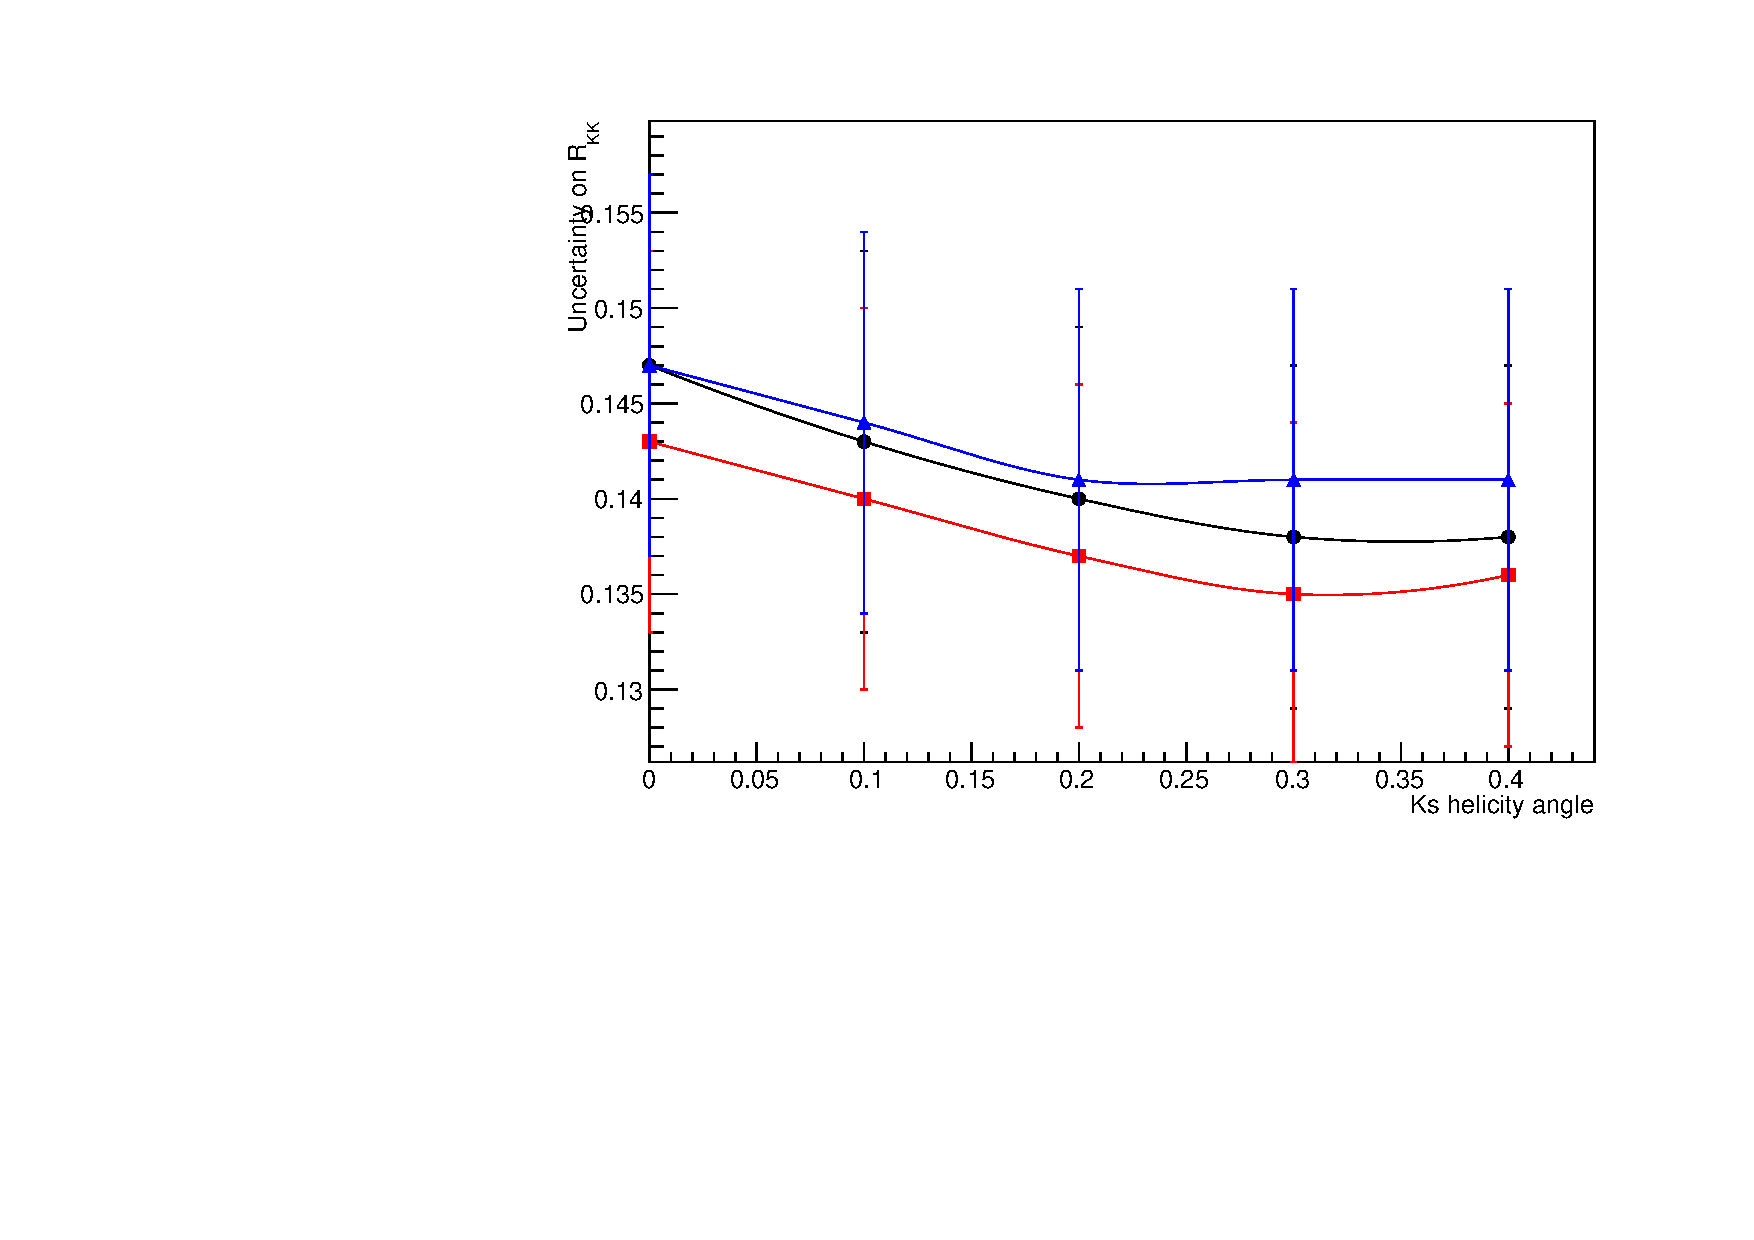
\includegraphics[width=\linewidth]{figures/selection/optimisation.pdf}
\caption{Value of the uncertainty on $R_{KK}$ as a function of \KS helicity angle selection for different \Kstar mass selections. The black curve is using a \Kstar mass window of 100 MeV, the red curve is using a \Kstar mass window of 75 MeV and the blue curve is using a \Kstar mass window of 50 MeV. The minimum uncertainty is given for a \Kstar mass window of 75 MeV and \KS helicity angle of 0.3. This was the \Kstar selection chosen after investigating uncertainties in other variables}
\label{optimisation}
\end{figure}

\begin{figure}
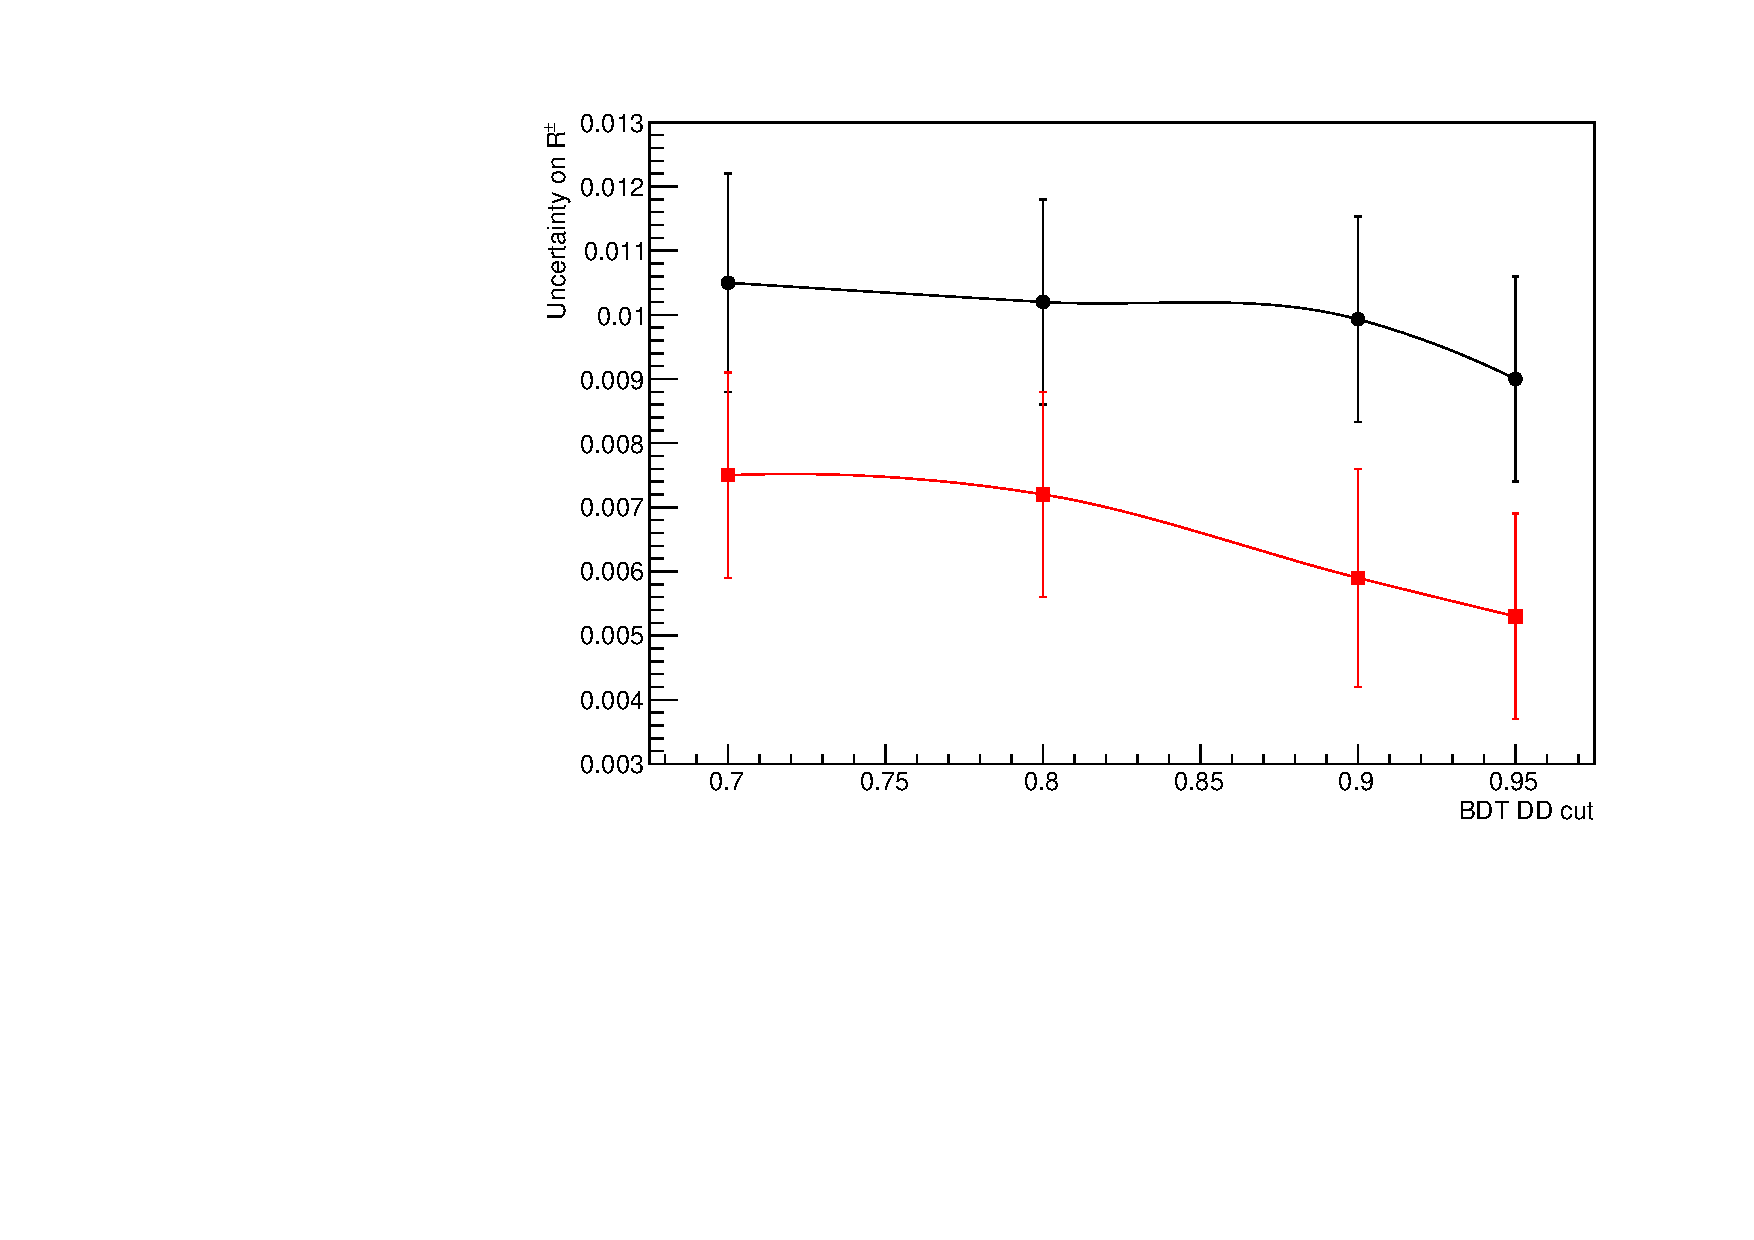
\includegraphics[width=\linewidth]{figures/selection/ADSoptimisation.pdf}
\caption{Value of the uncertainty on $R^+$ and $R^-$ as a function of BDT\_DD cut in the ADS mode. These toys were run with a BDT LL cut of 0.6 on all modes and BDT DD cut of 0.7 on all modes other than the ADS. The black curve is the uncertainty of $R^+$ and the red curve is the uncertainty of $R^-$. Although the uncertainty continues to decrease for a BDT cut of 0.95, this resulted in a significant drop in signal efficiency, therefore a cut of 0.9 was chosen for the ADS}
\label{adsoptimisation}
\end{figure}

The final selection chosen was:

\begin{itemize}
\item{75 MeV \Kstar mass window}
\item{\textbar cos(\KS helicity angle) \textbar $>$ 0.3}
\item{BDT $>$ 0.6 for LL and 0.7 for DD, except in the ADS mode where BDT $>$ 0.6 for LL and 0.9 for DD}
\end{itemize}

The choice of BDT selection in ADS mode remains optimal when tested against a scenario of low combinatoric in the ADS mode. 

%%%%%%%%%%%%%%%%%%%%%%%%
\subsection{Fit results}
\label{sec:cpfit:results}

The fits to data are shown in Figures \ref{datafit2bodyRun1}, \ref{datafit4bodyRun1}, \ref{datafit2bodyRun2} and \ref{datafit4bodyRun2}. The \CP oberservables measured from the fit are below, where the first errors are statistical and the second are systematic.

\begin{align*}
A_{K\pi} & = -0.004 \pm 0.023 \pm 0.008 \\
A_{KK} & = 0.06 \pm 0.07 \pm 0.01 \\
A_{\pi\pi} & = 0.15 \pm 0.13 \pm 0.02 \\
R_{KK} & = 1.24 \pm 0.09 \pm 0.01 \\
R_{\pi\pi} & = 1.08 \pm 0.15 \pm 0.03 \\
R^+_{K\pi} & = 0.020 \pm 0.006 \pm 0.001 \\
R^-_{K\pi} & = 0.002 \pm 0.004 \pm 0.001 \\
A_{K\pi\pi\pi} & = -0.013 \pm 0.031 \pm 0.009 \\
A_{\pi\pi\pi\pi} & = 0.03 \pm 0.11 \pm 0.01 \\
R_{\pi\pi\pi\pi} & = 1.11 \pm 0.13 \pm 0.03 \\
R^+_{K\pi\pi\pi} & = 0.016 \pm 0.008 \pm 0.003 \\
R^-_{K\pi\pi\pi} & = 0.006 \pm 0.007 \pm 0.004 \\
\end{align*}

\begin{sidewaysfigure}[h]
\centering
\subfloat[$K\pi$, LL]{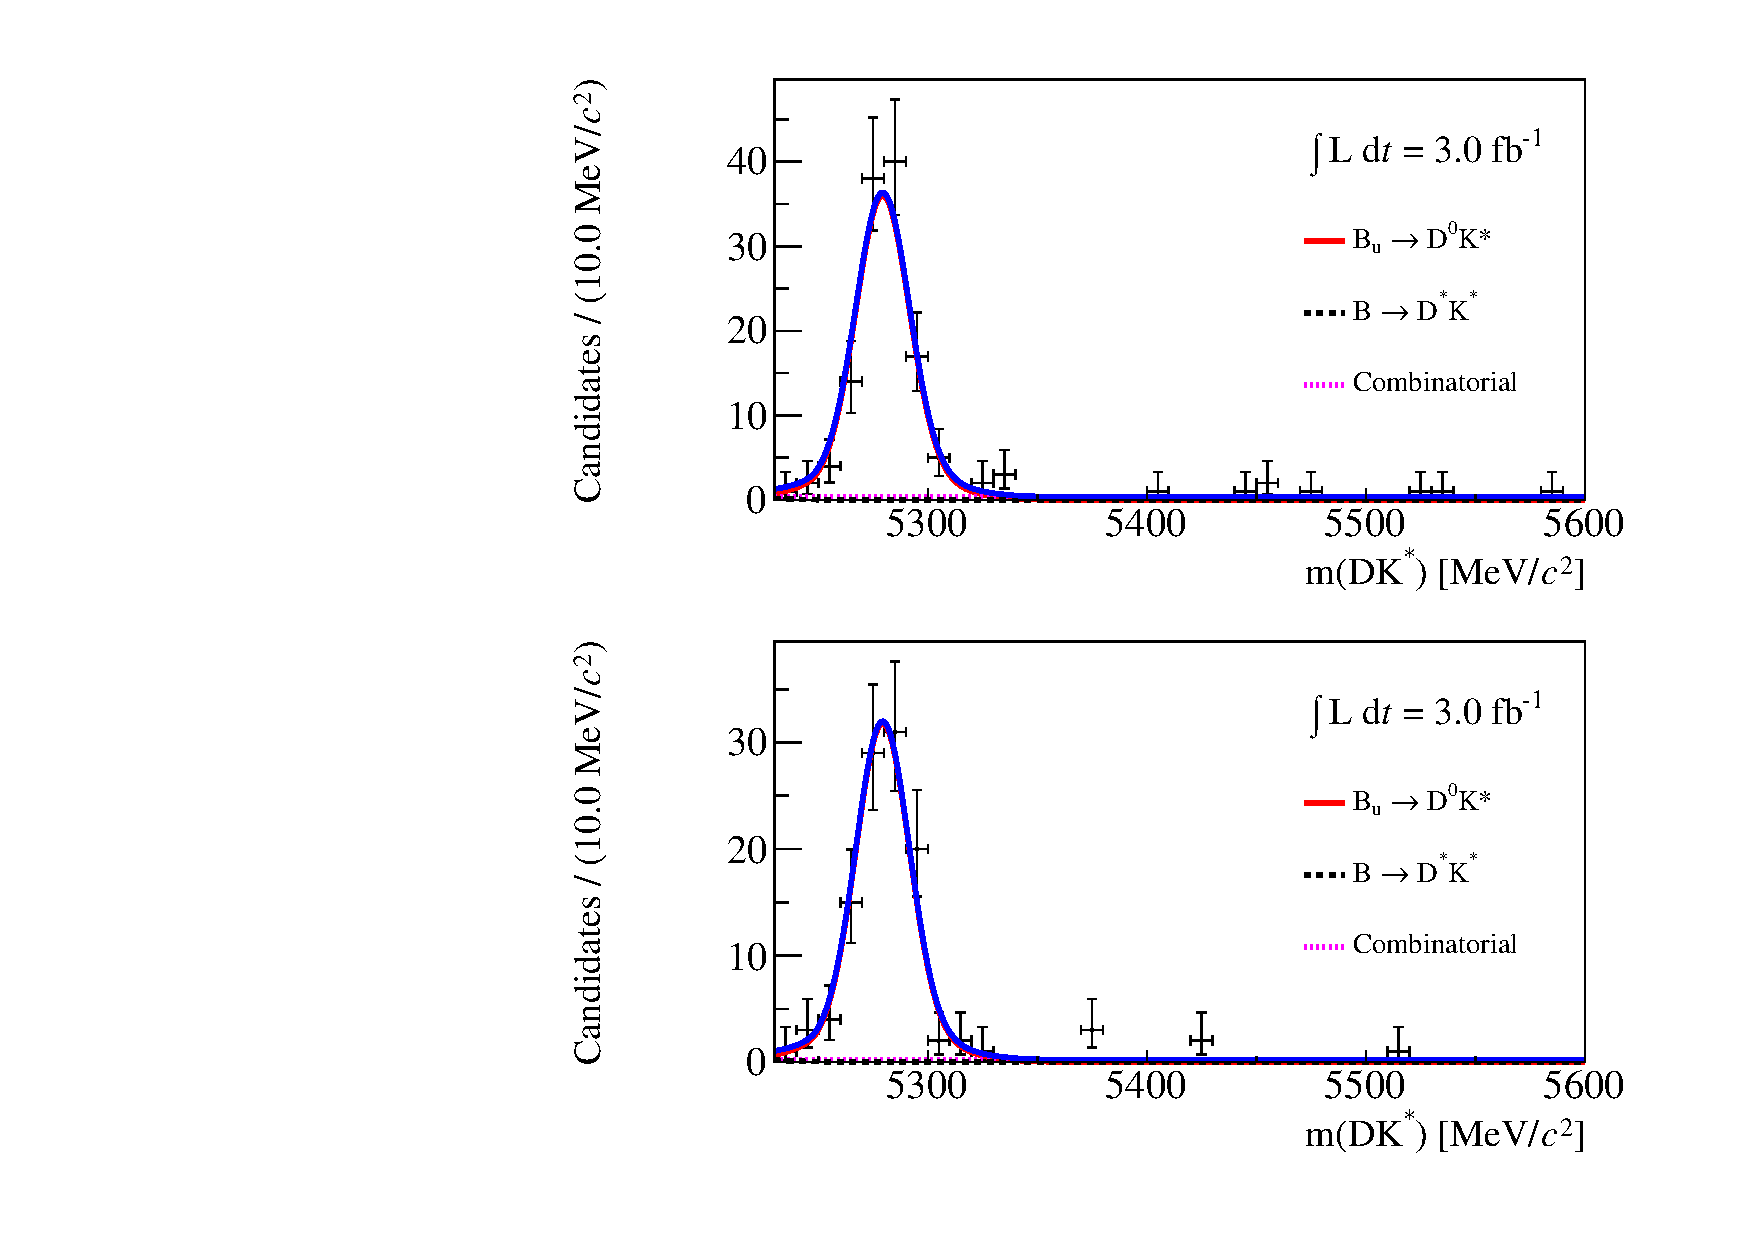
\includegraphics[width=0.25\linewidth]{figures/results/canvas_d2kpi_LL_run1.pdf}}
\hfill
\subfloat[$KK$, LL]{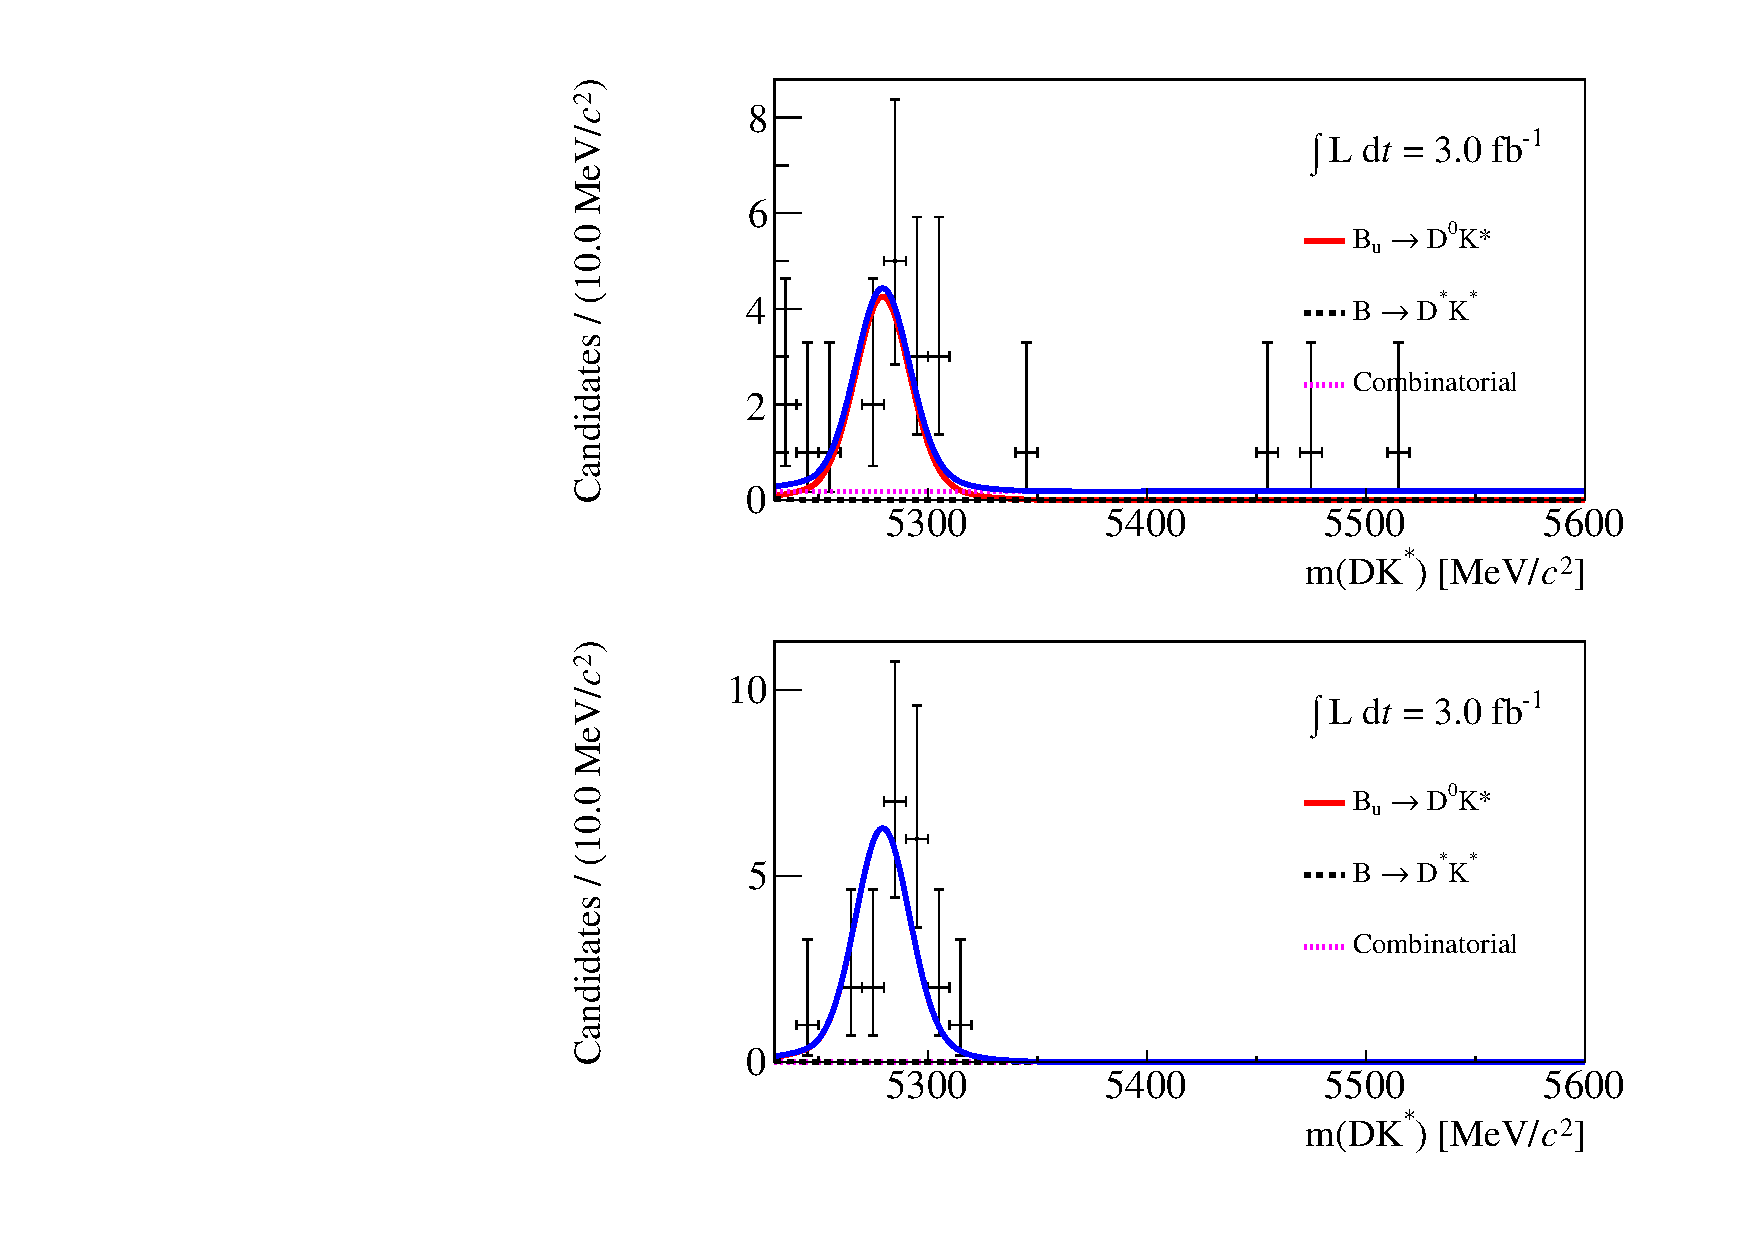
\includegraphics[width=0.25\linewidth]{figures/results/canvas_d2kk_LL_run1.pdf}}
\hfill
\subfloat[$\pi\pi$, LL]{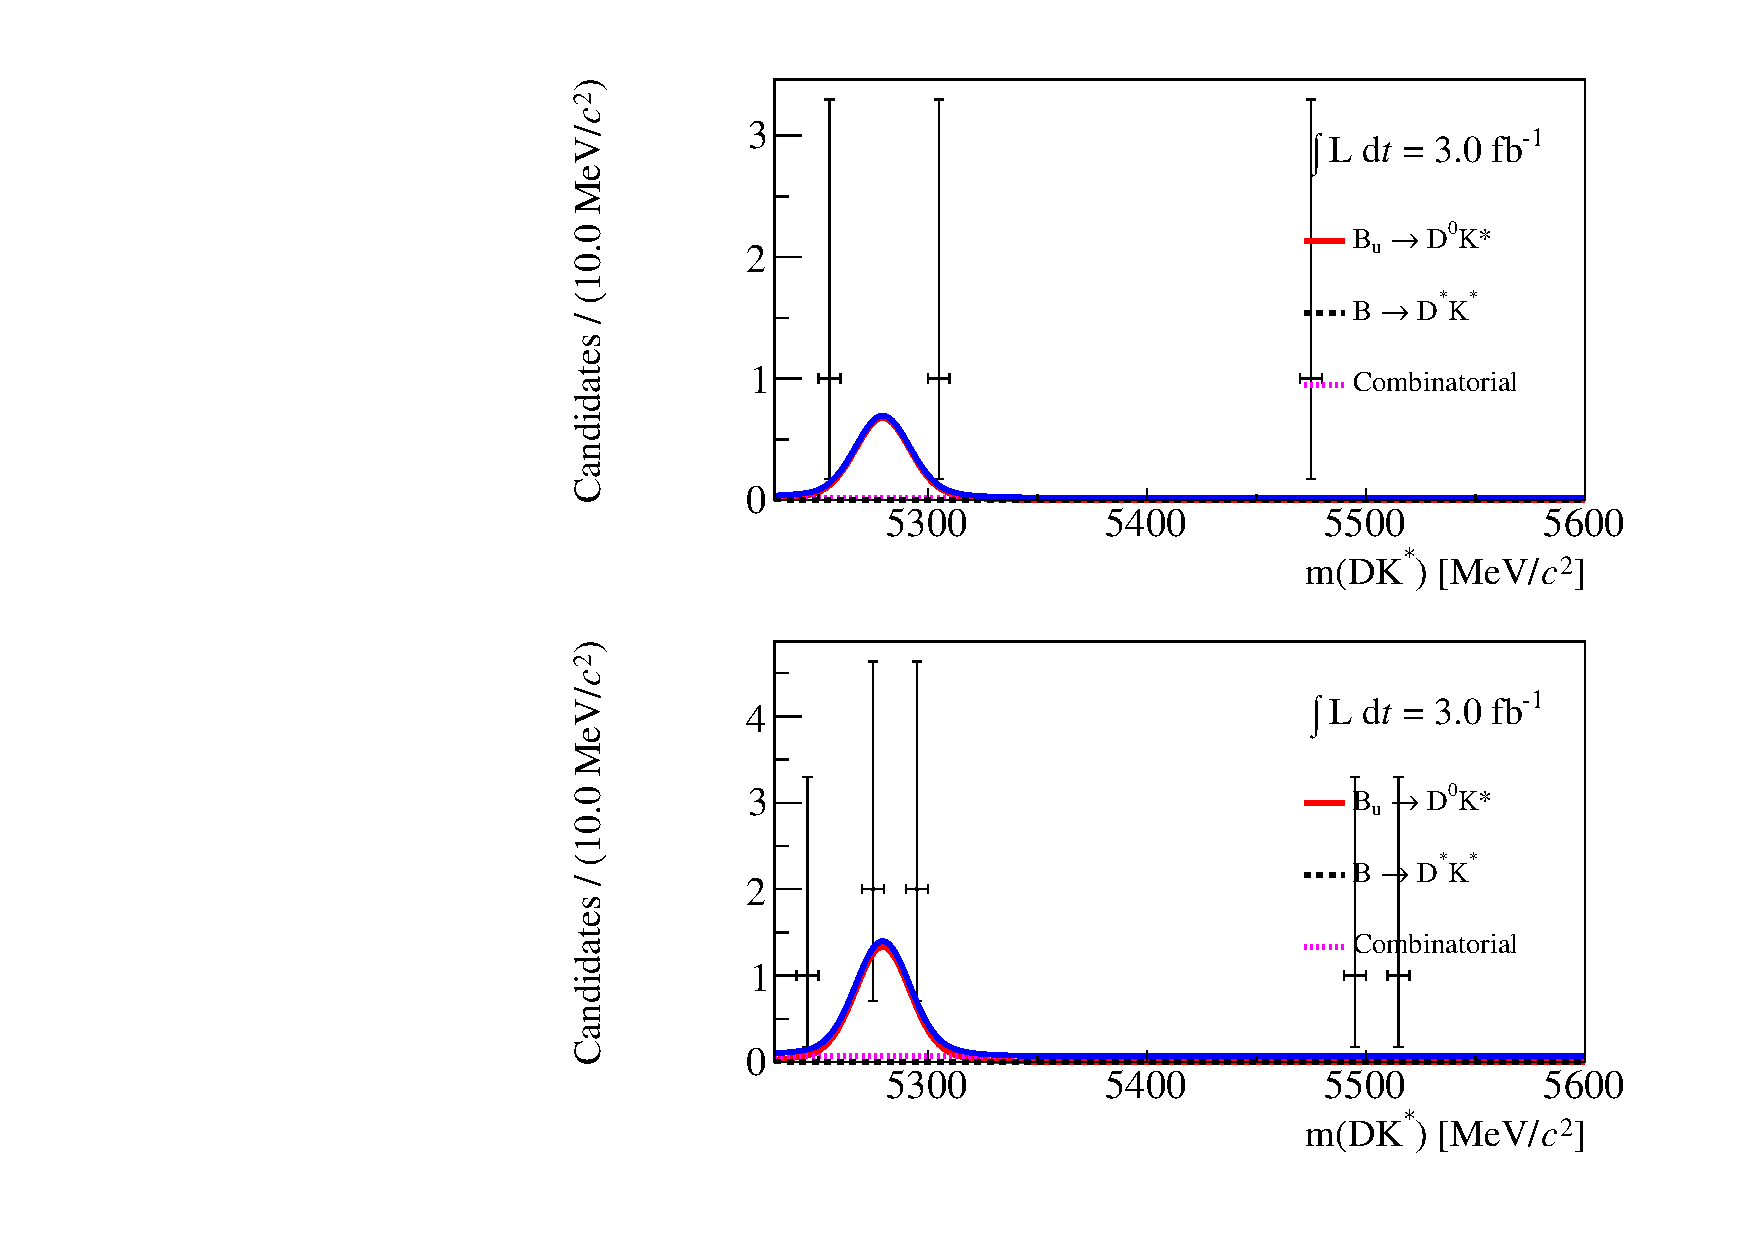
\includegraphics[width=0.25\linewidth]{figures/results/canvas_d2pipi_LL_run1.pdf}}
\hfill
\subfloat[$\pi K$, LL]{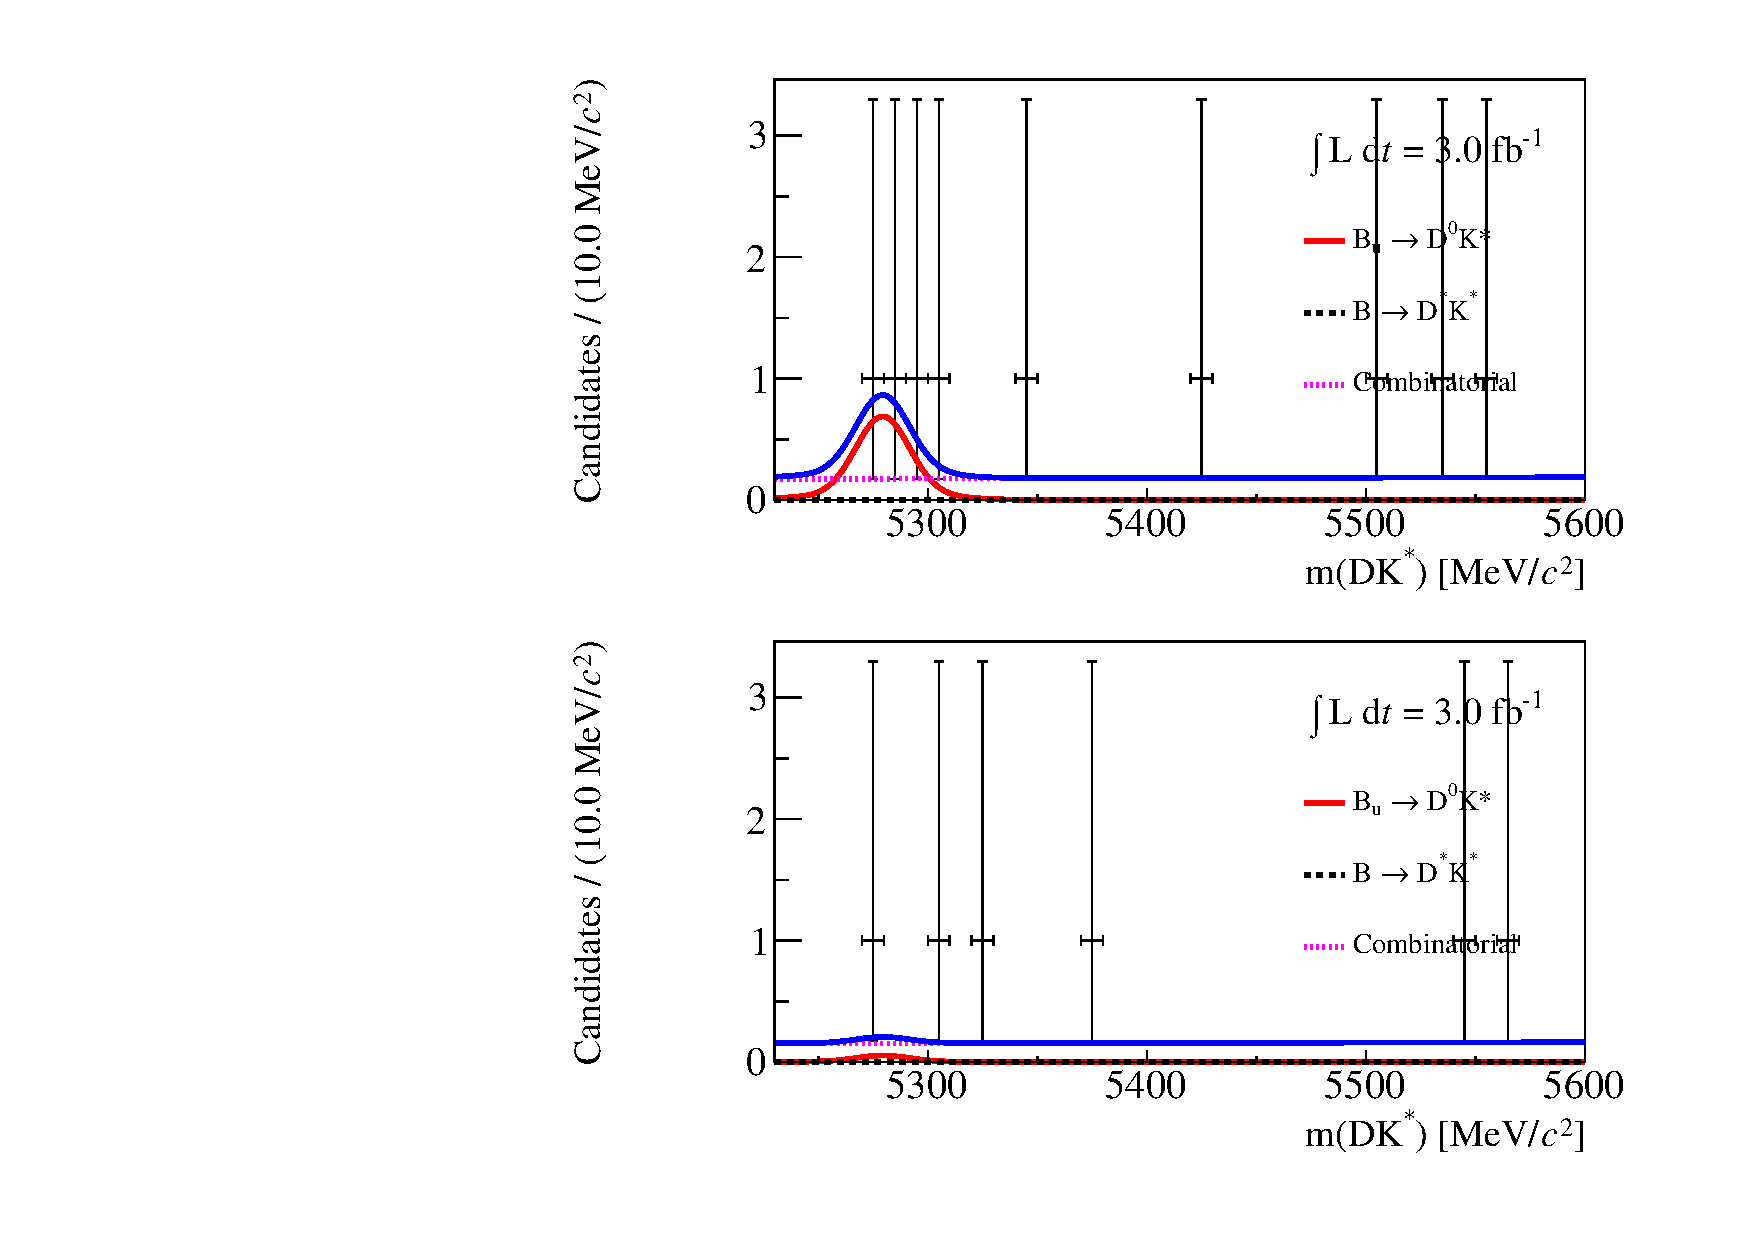
\includegraphics[width=0.25\linewidth]{figures/results/canvas_d2pik_LL_run1.pdf}}
\hfill
\subfloat[$K\pi$, DD]{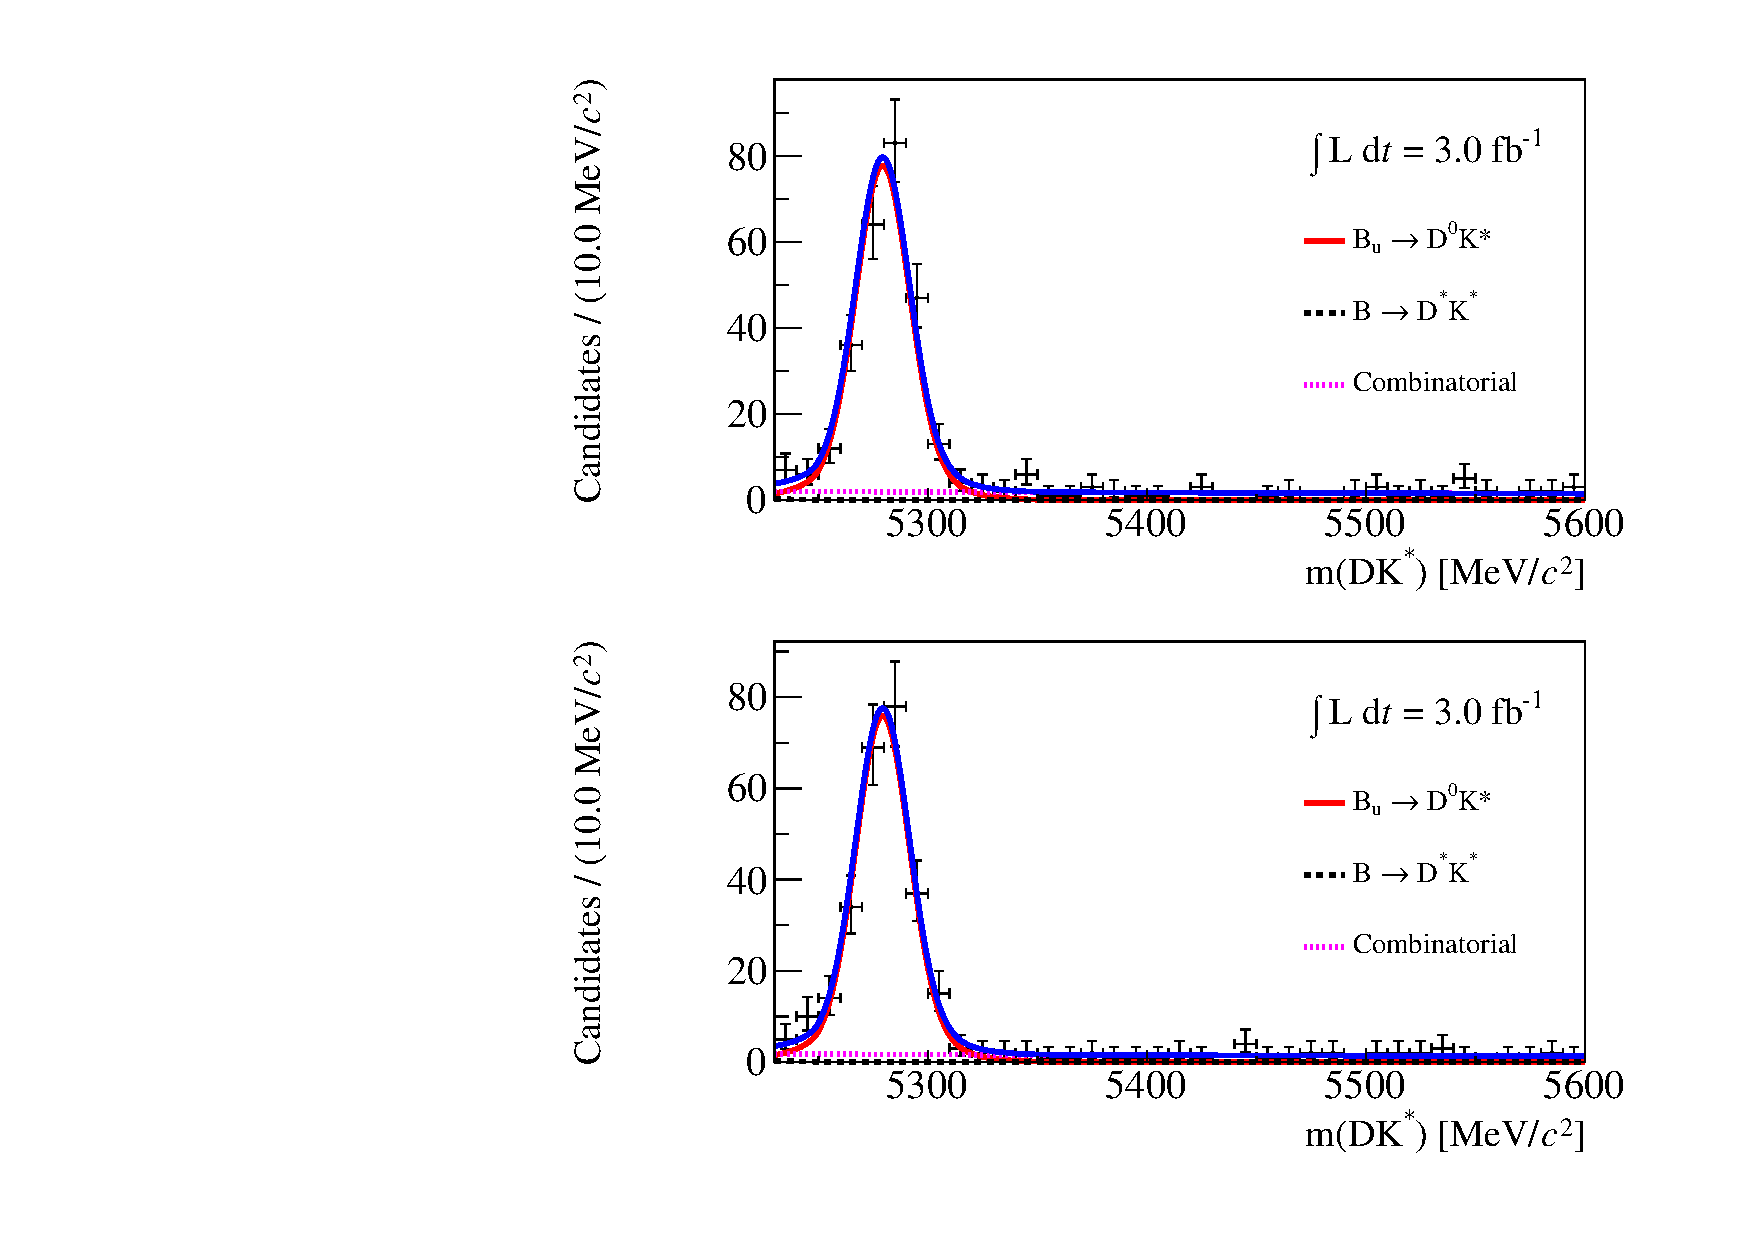
\includegraphics[width=0.25\linewidth]{figures/results/canvas_d2kpi_DD_run1.pdf}}
\hfill
\subfloat[$KK$, DD]{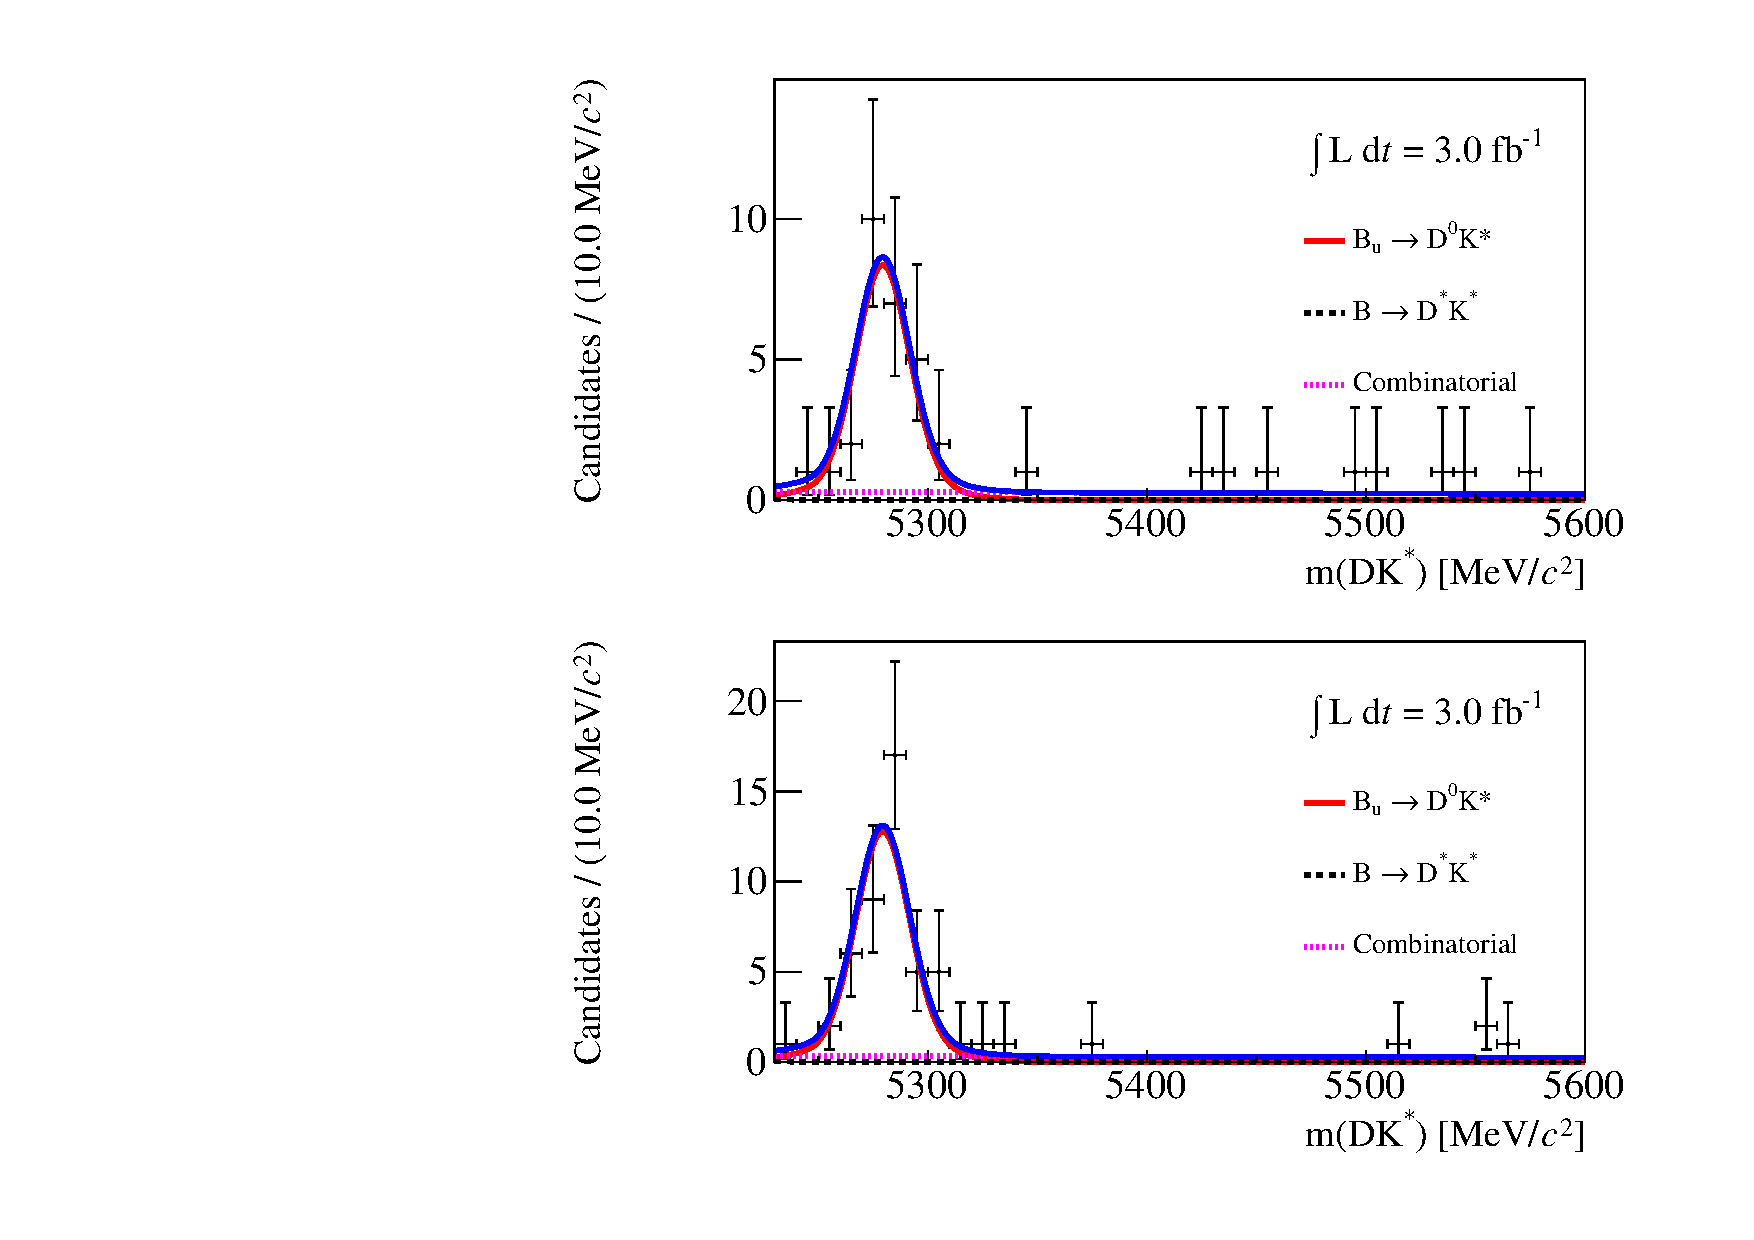
\includegraphics[width=0.25\linewidth]{figures/results/canvas_d2kk_DD_run1.pdf}}
\hfill
\subfloat[$\pi\pi$, DD]{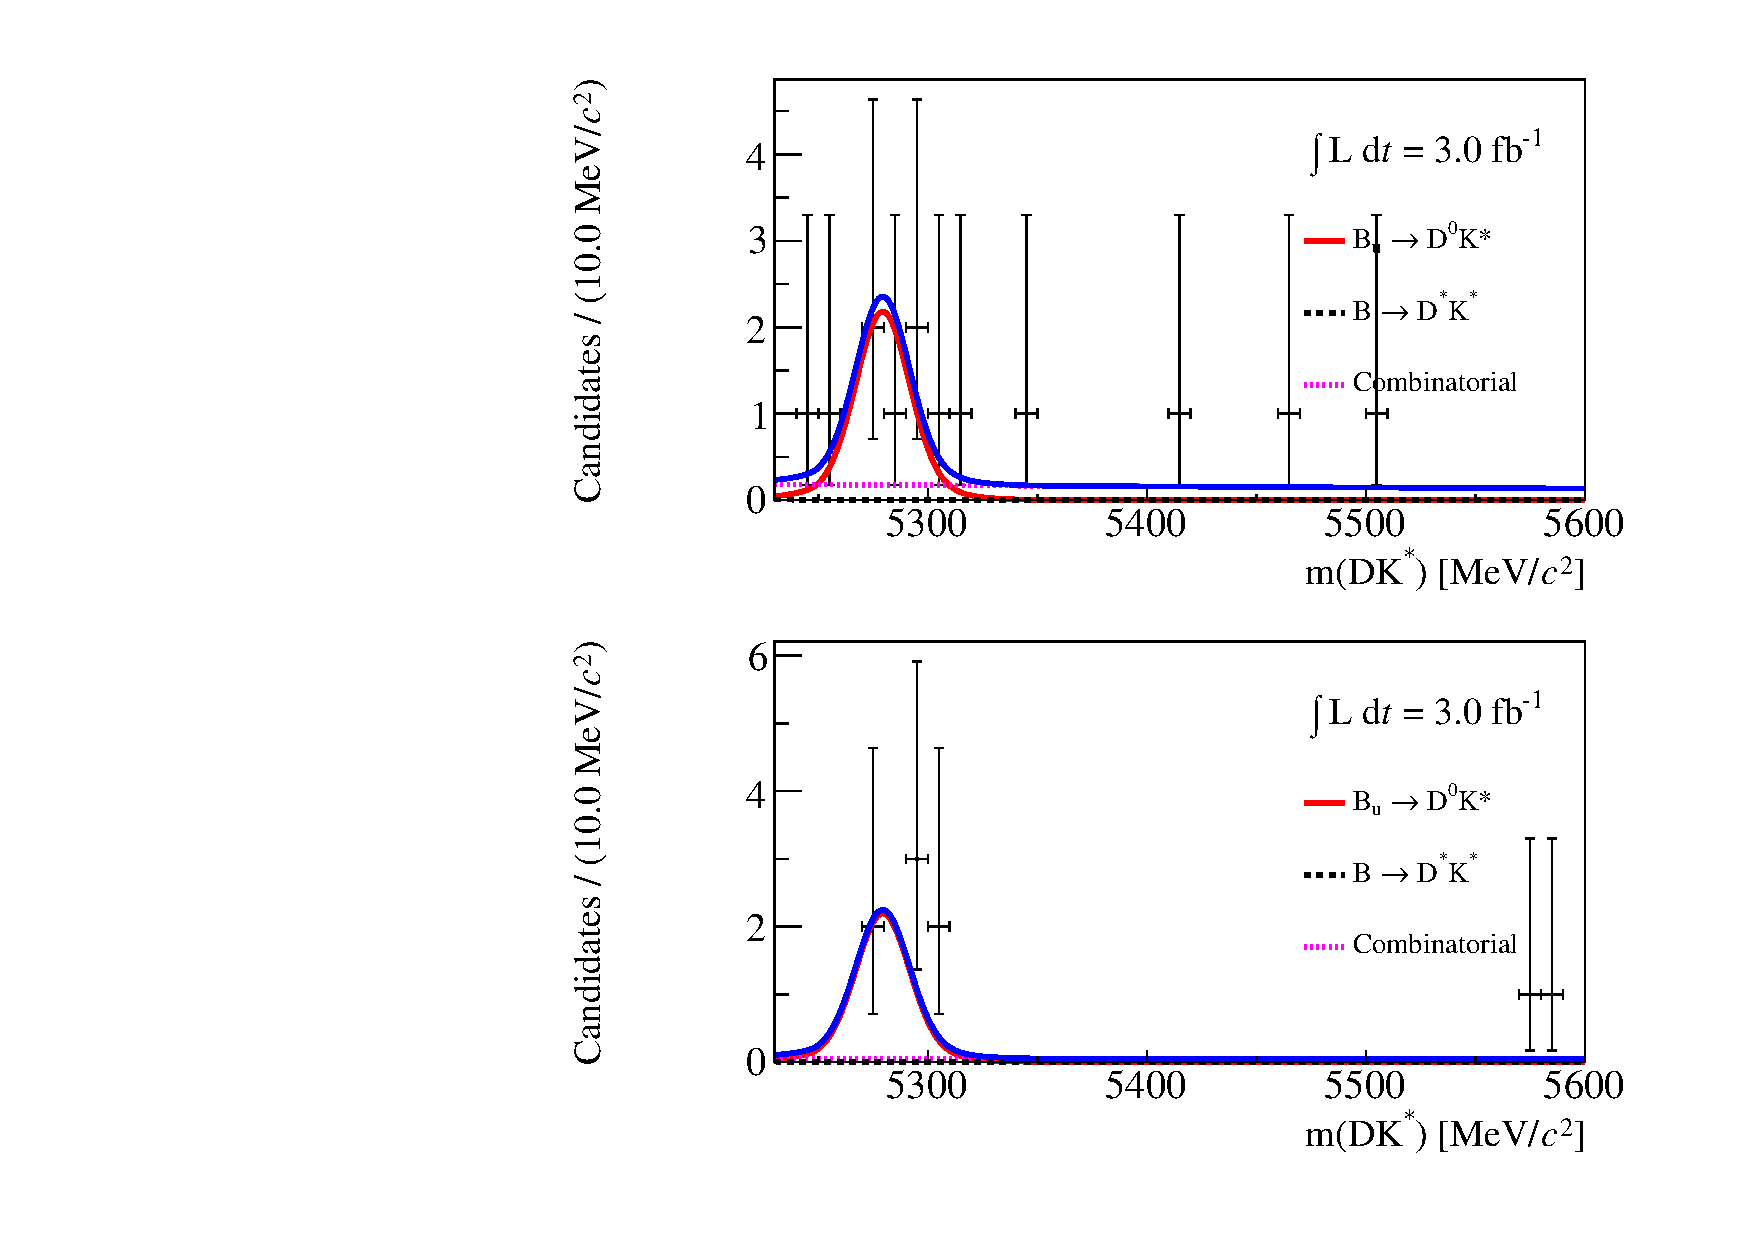
\includegraphics[width=0.25\linewidth]{figures/results/canvas_d2pipi_DD_run1.pdf}}
\hfill
\subfloat[$\pi K$, DD]{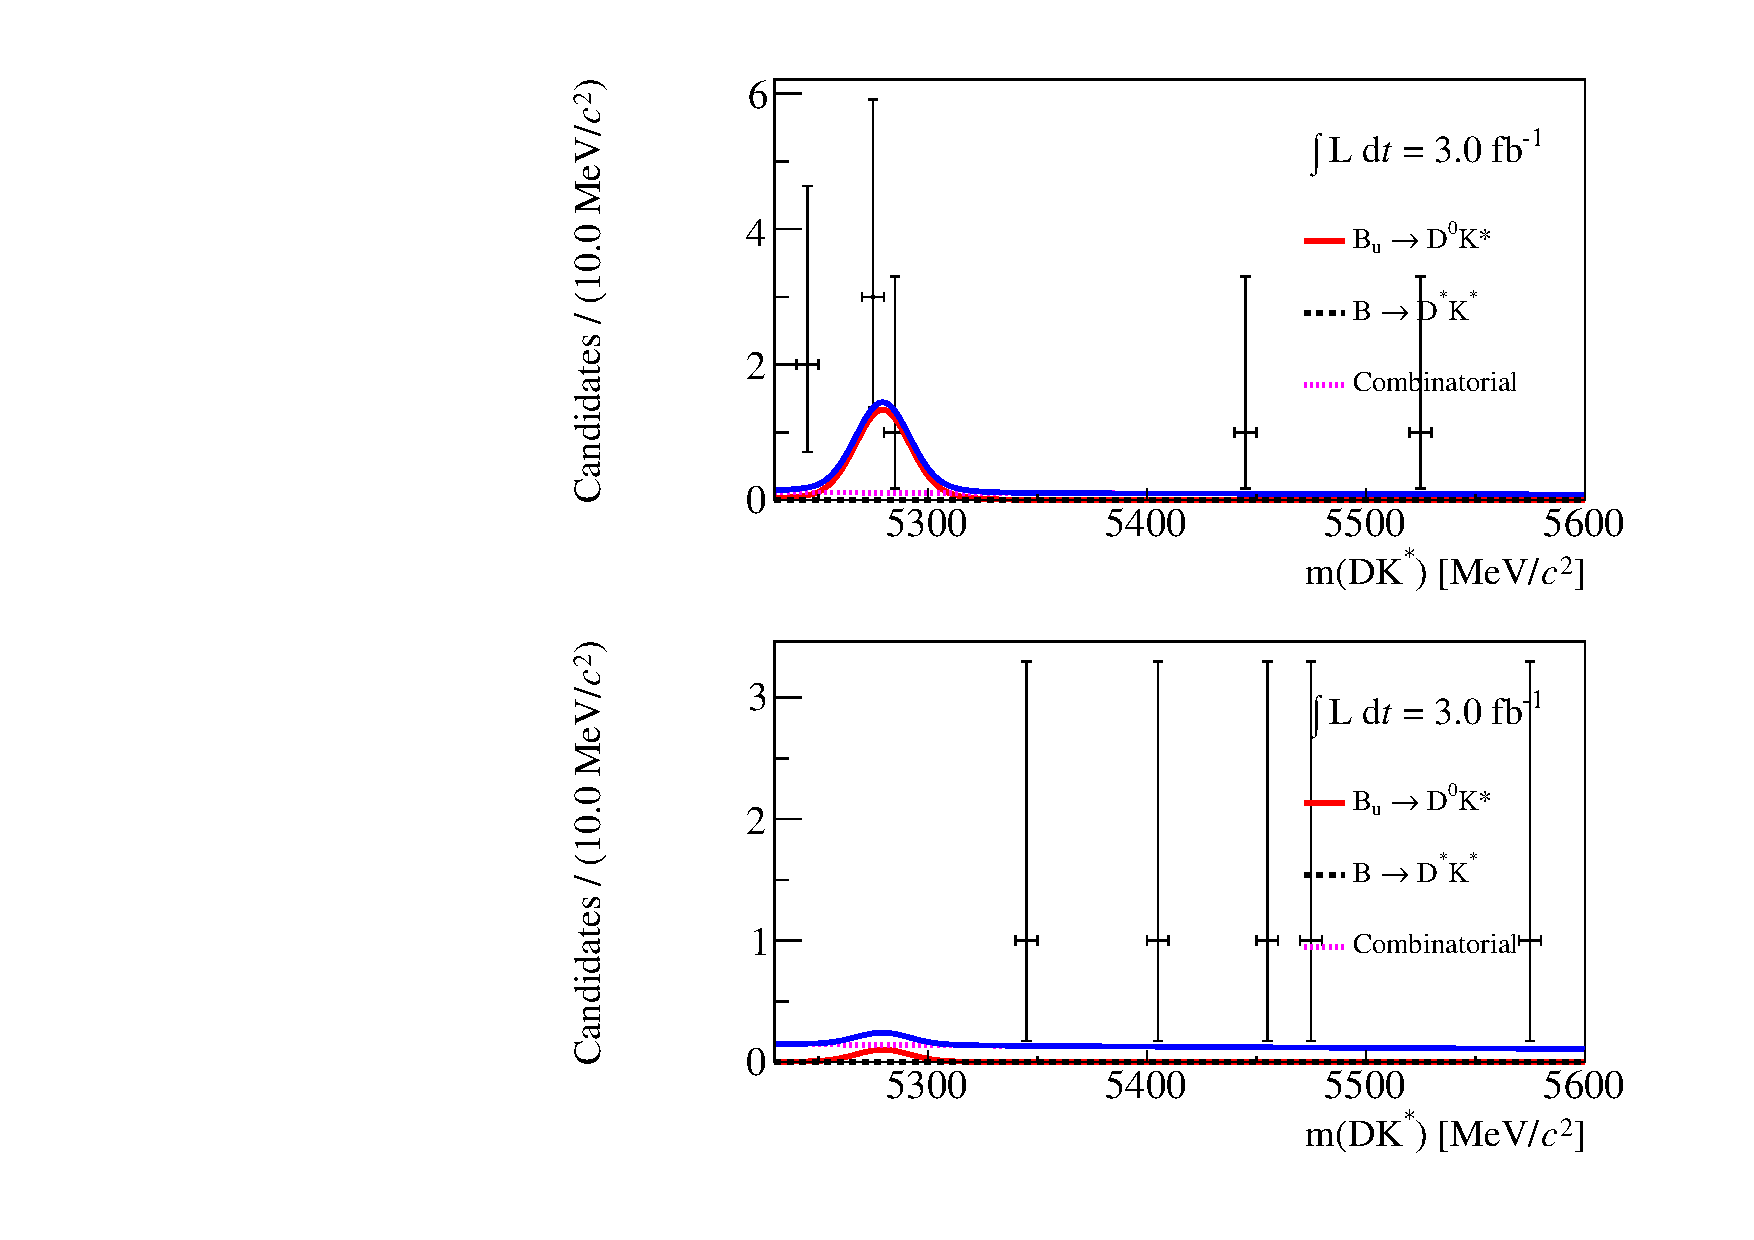
\includegraphics[width=0.25\linewidth]{figures/results/canvas_d2pik_DD_run1.pdf}}
\caption{Results of the simultaneous fit for Run 1 data for 2-body modes. In each pair the top plot is for \Bp decays and the bottom plot is for \Bm decays.}
\label{datafit2bodyRun1}
\end{sidewaysfigure}

\begin{sidewaysfigure}[h]
\centering
\subfloat[$K\pi\pi\pi$, LL]{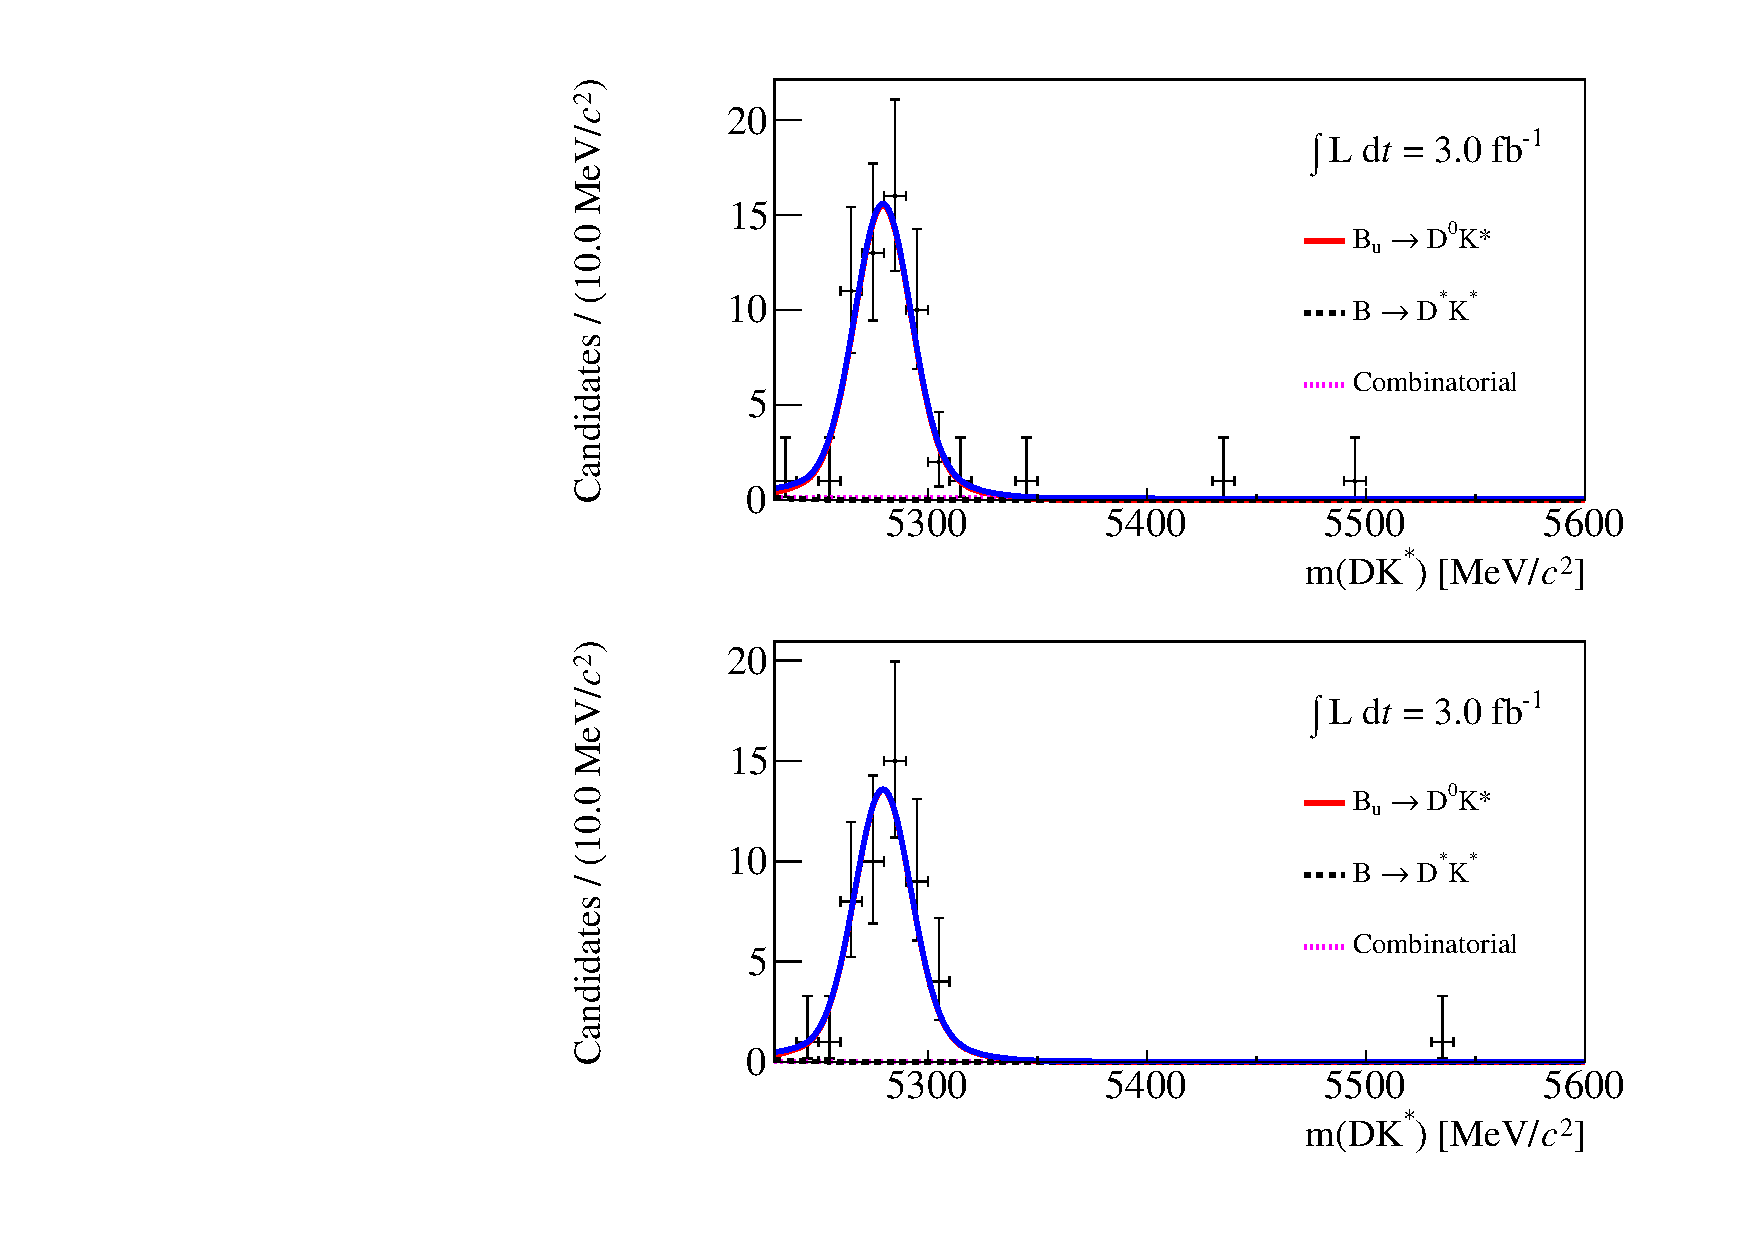
\includegraphics[width=0.3\linewidth]{figures/results/canvas_d2kpipipi_LL_run1.pdf}}
\hfill
\subfloat[$\pi\pi\pi\pi$, LL]{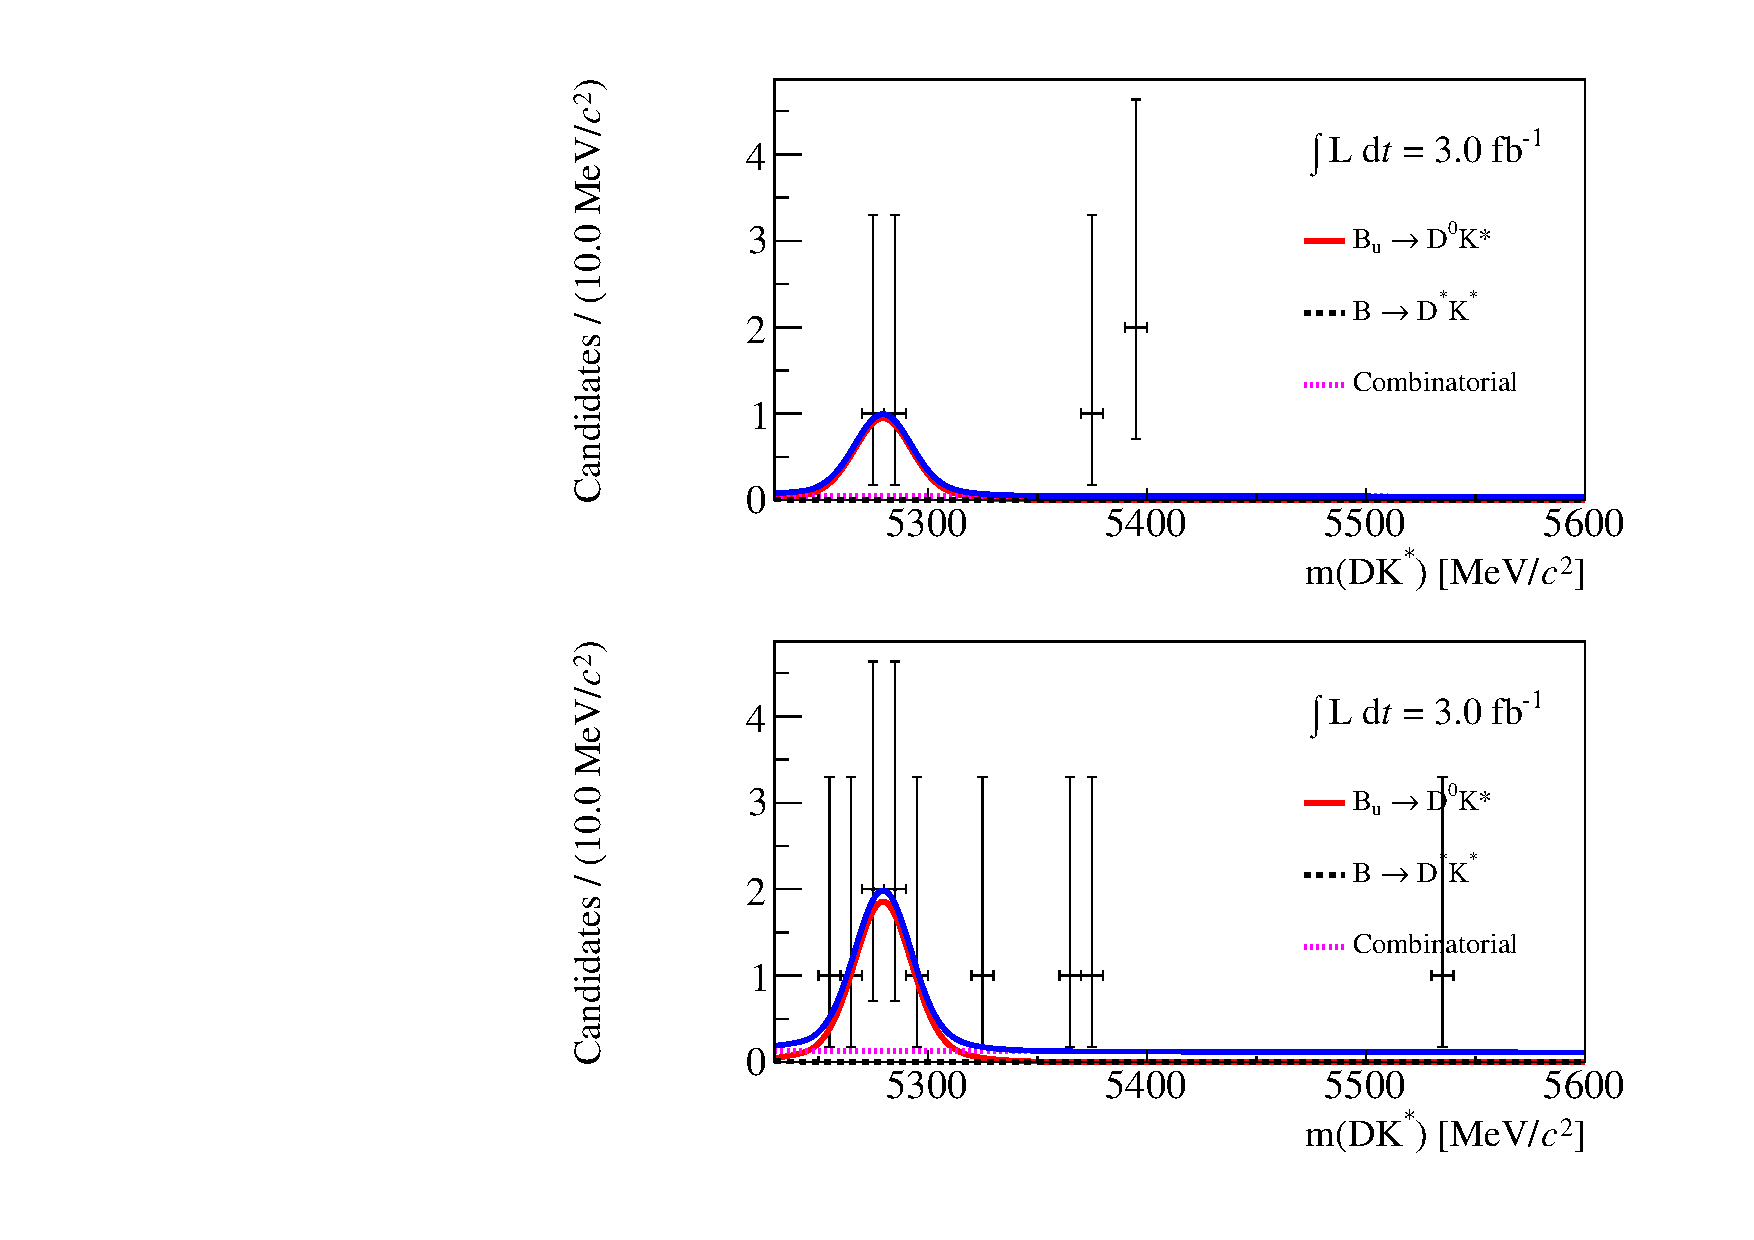
\includegraphics[width=0.3\linewidth]{figures/results/canvas_d2pipipipi_LL_run1.pdf}}
\hfill
\subfloat[$\pi K\pi\pi$, LL]{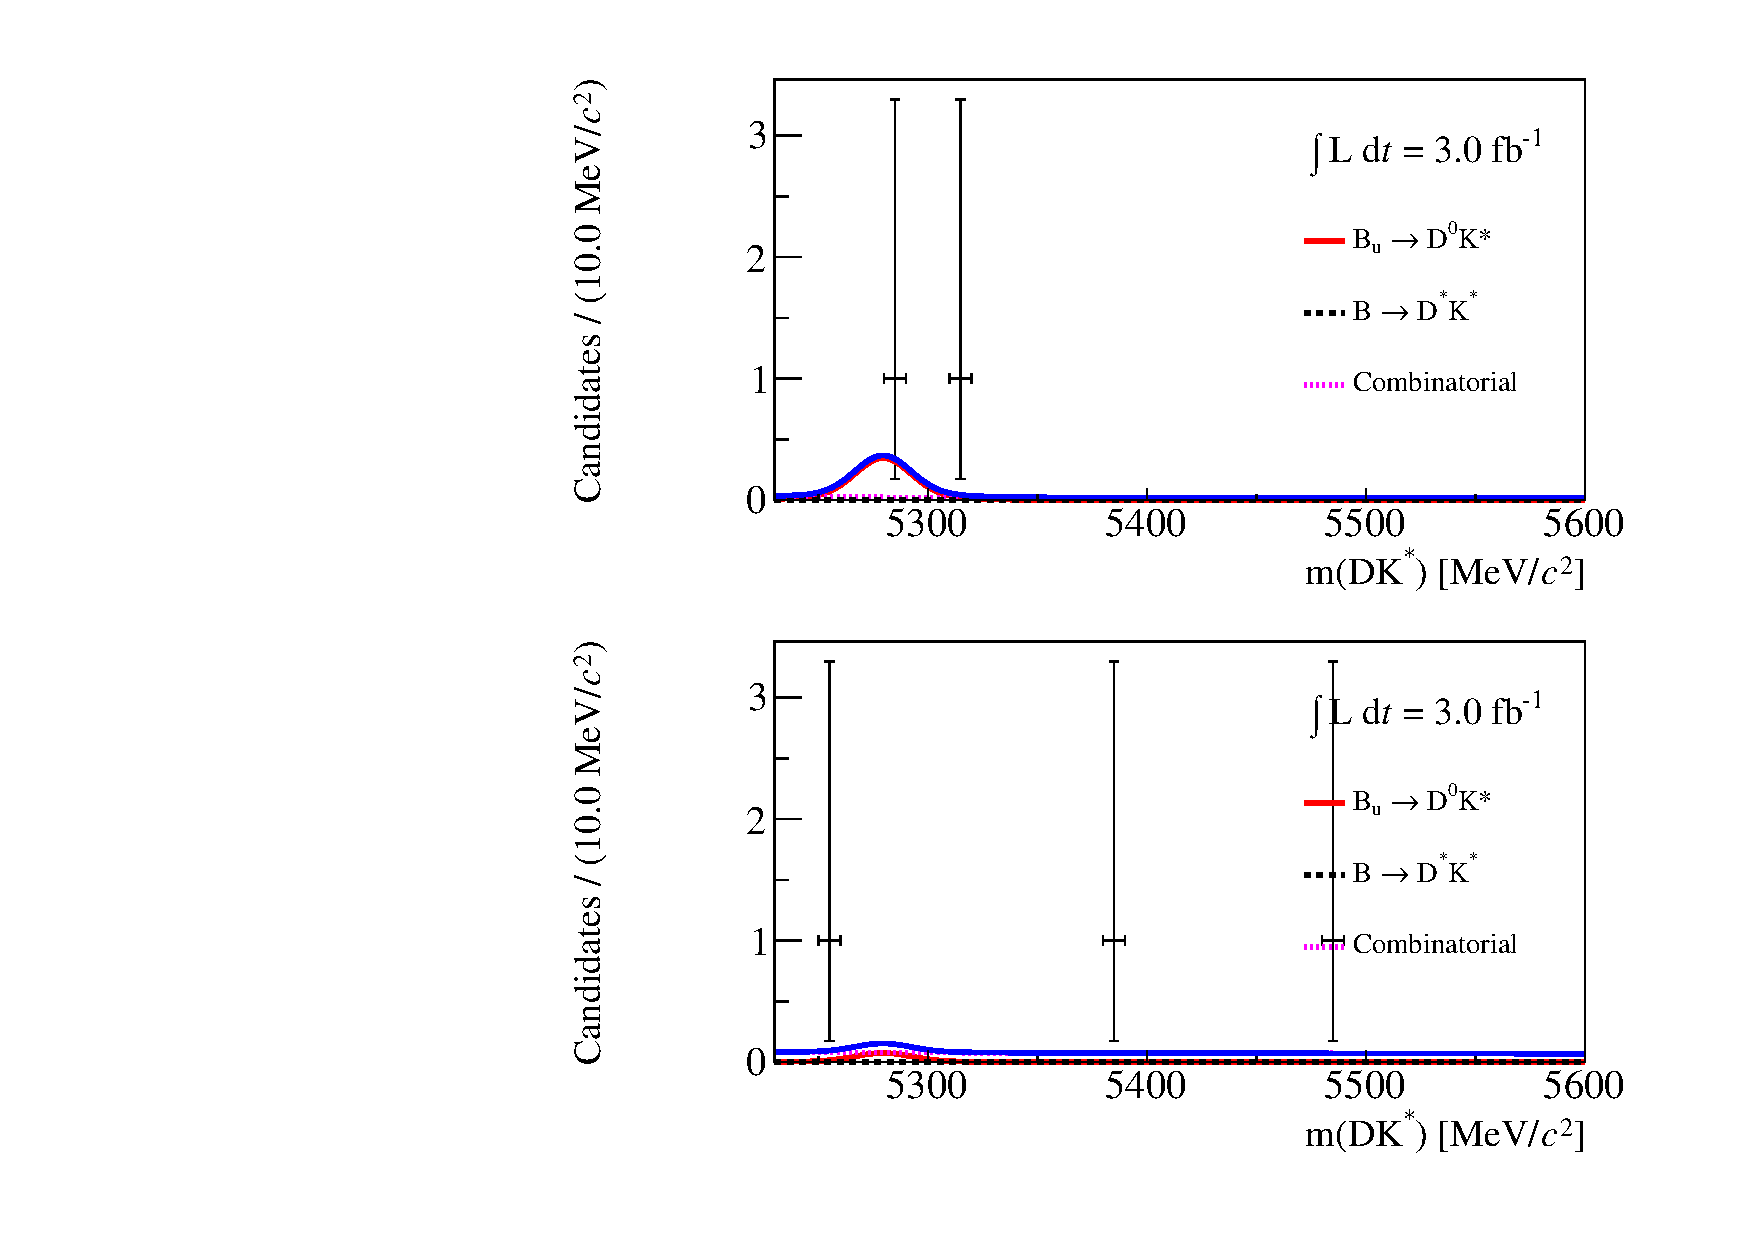
\includegraphics[width=0.3\linewidth]{figures/results/canvas_d2pikpipi_LL_run1.pdf}}
\hfill
\subfloat[$K\pi\pi\pi$, DD]{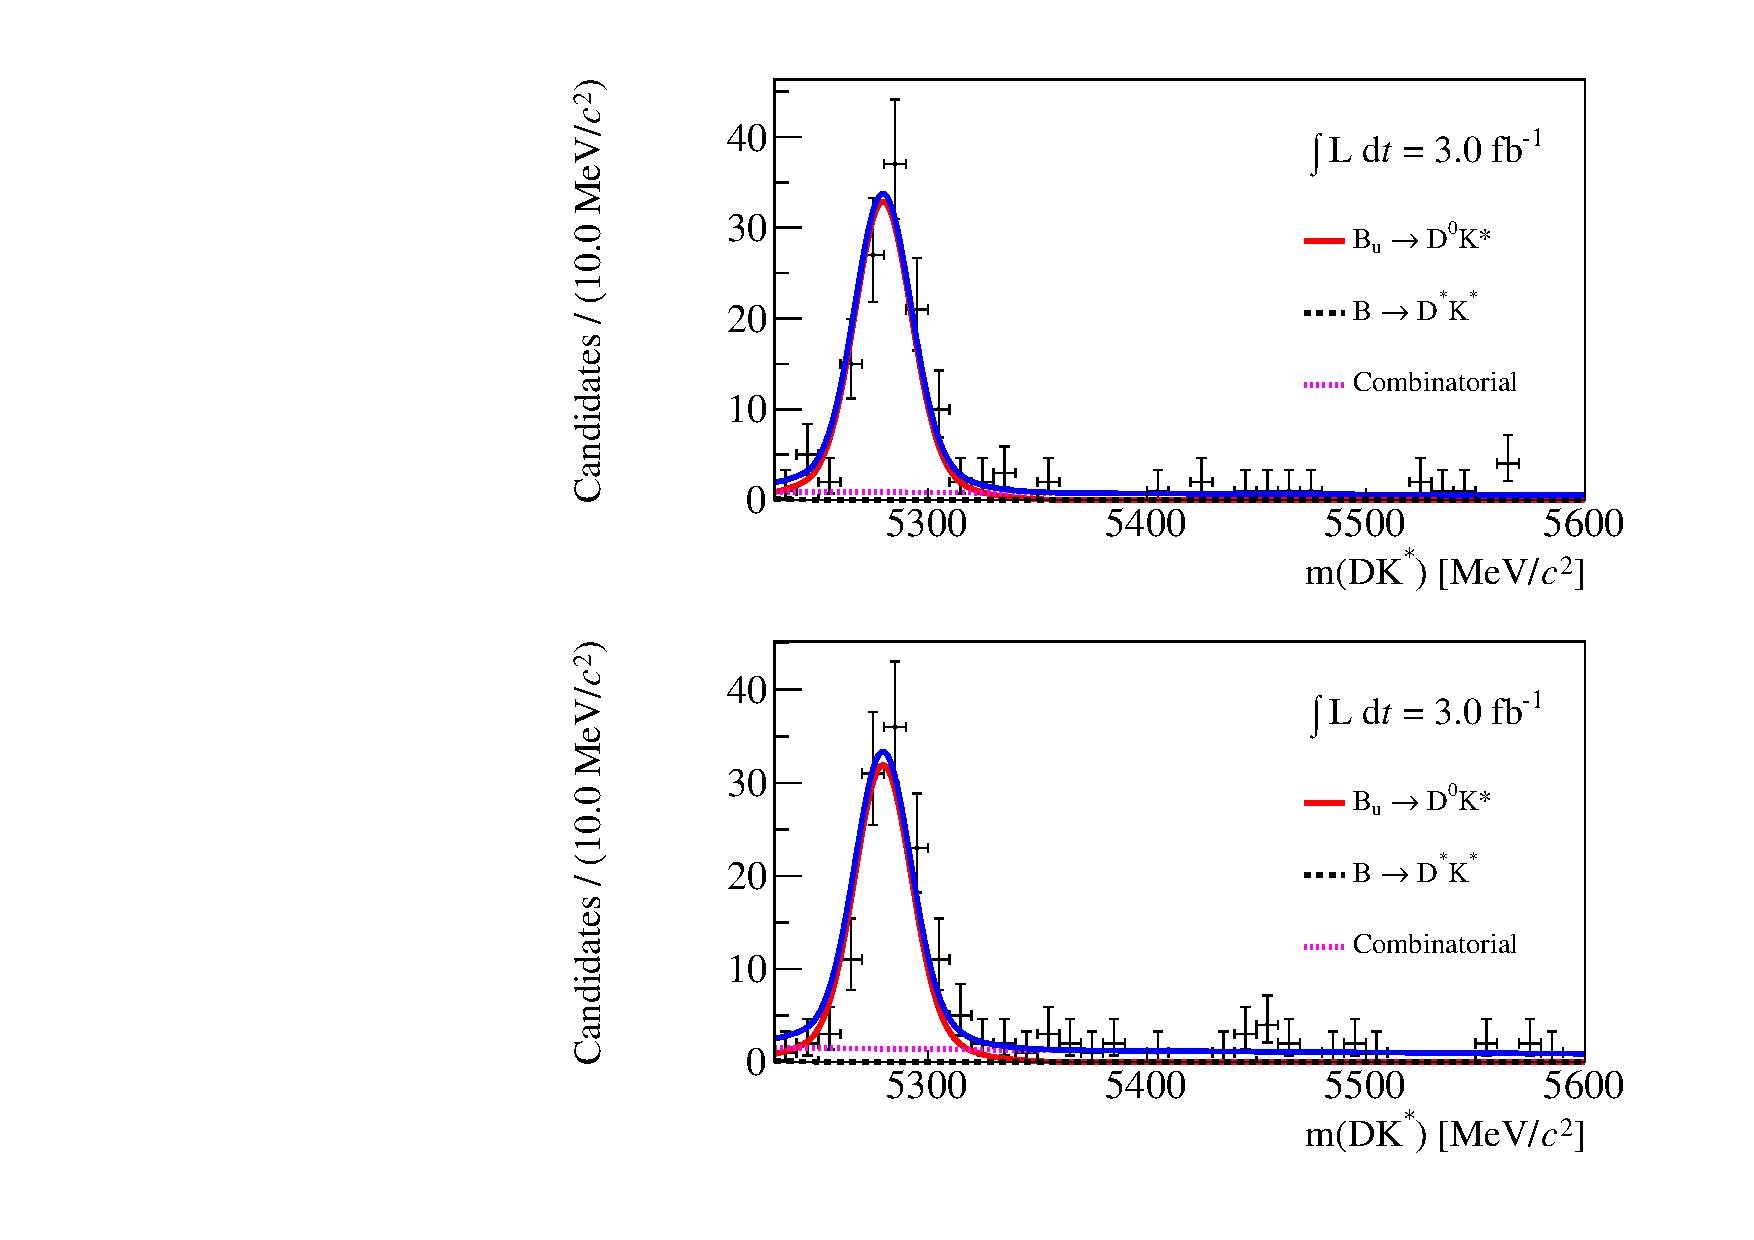
\includegraphics[width=0.3\linewidth]{figures/results/canvas_d2kpipipi_DD_run1.pdf}}
\hfill
\subfloat[$\pi\pi\pi\pi$, DD]{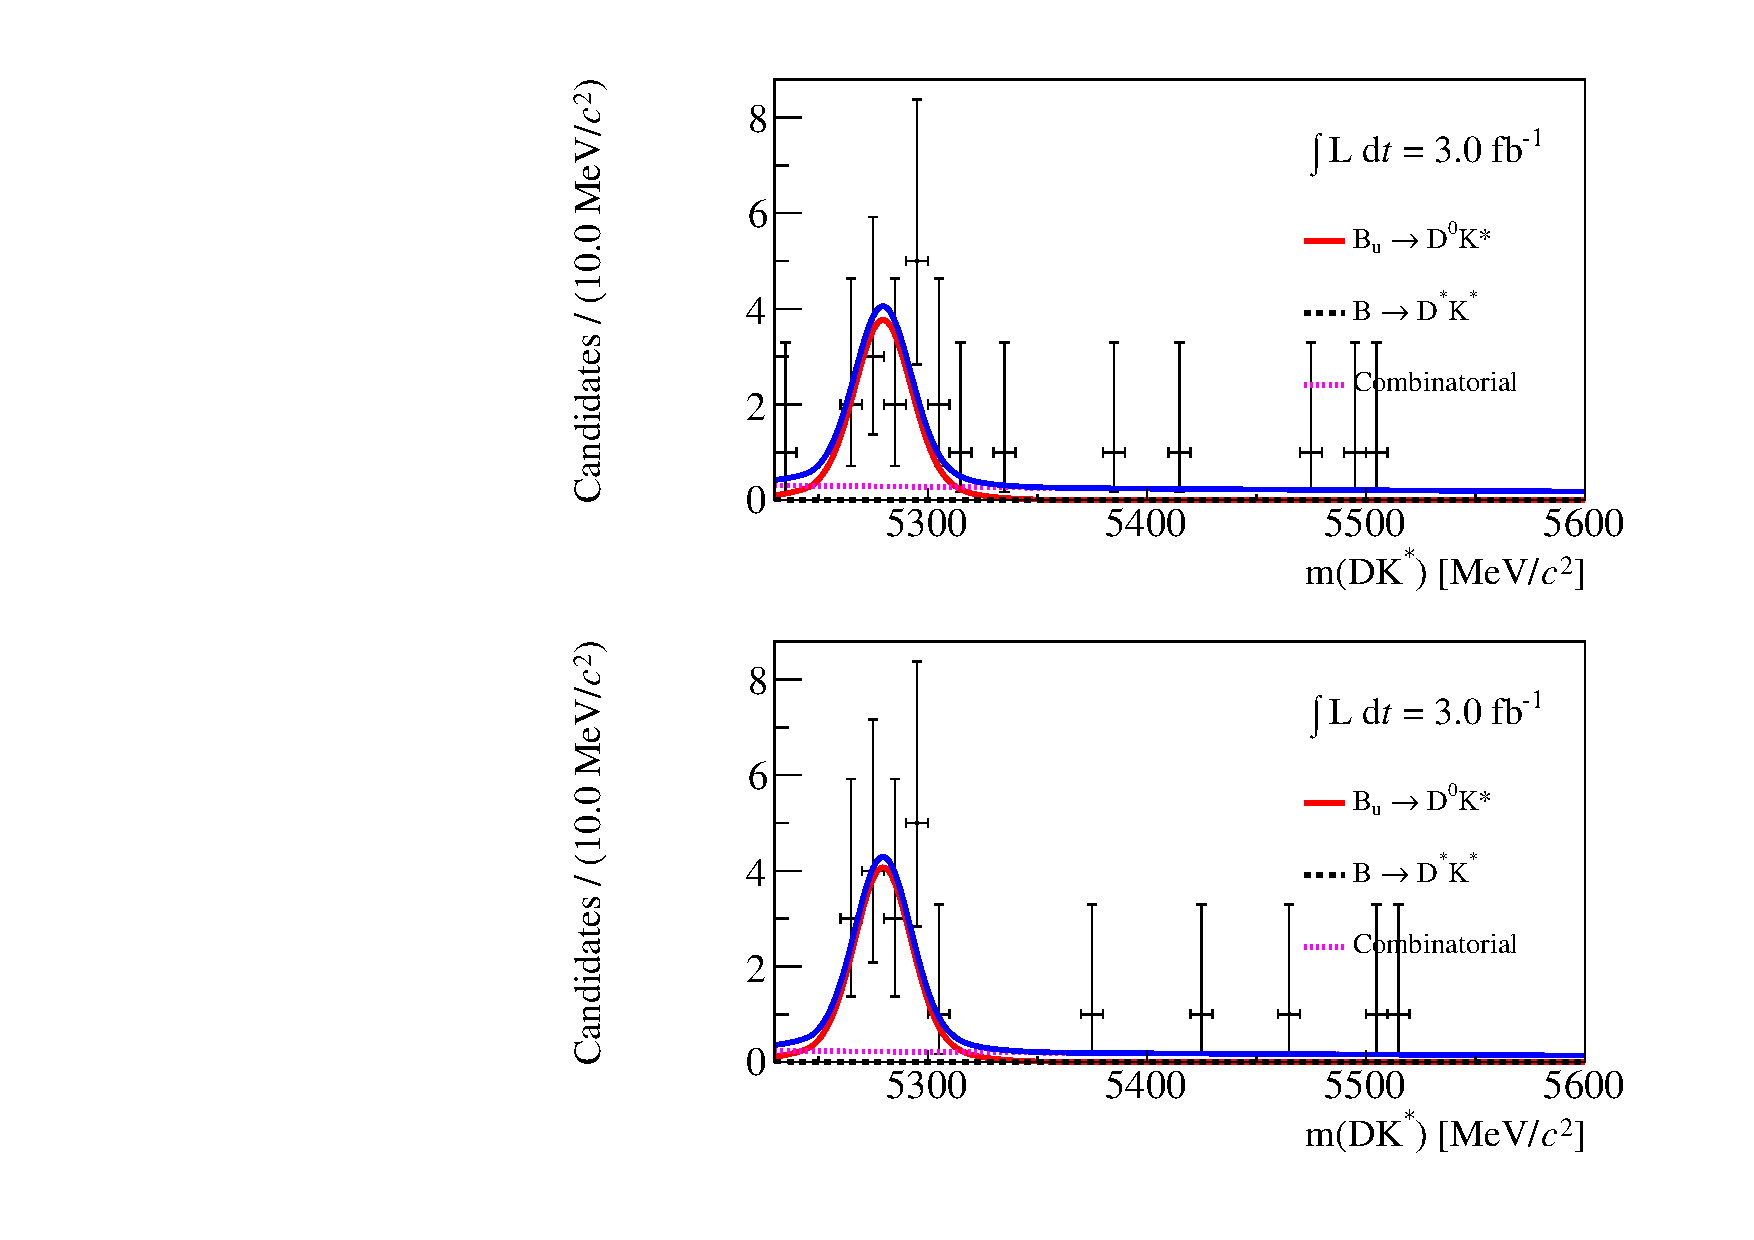
\includegraphics[width=0.3\linewidth]{figures/results/canvas_d2pipipipi_DD_run1.pdf}}
\hfill
\subfloat[$\pi K\pi\pi$, DD]{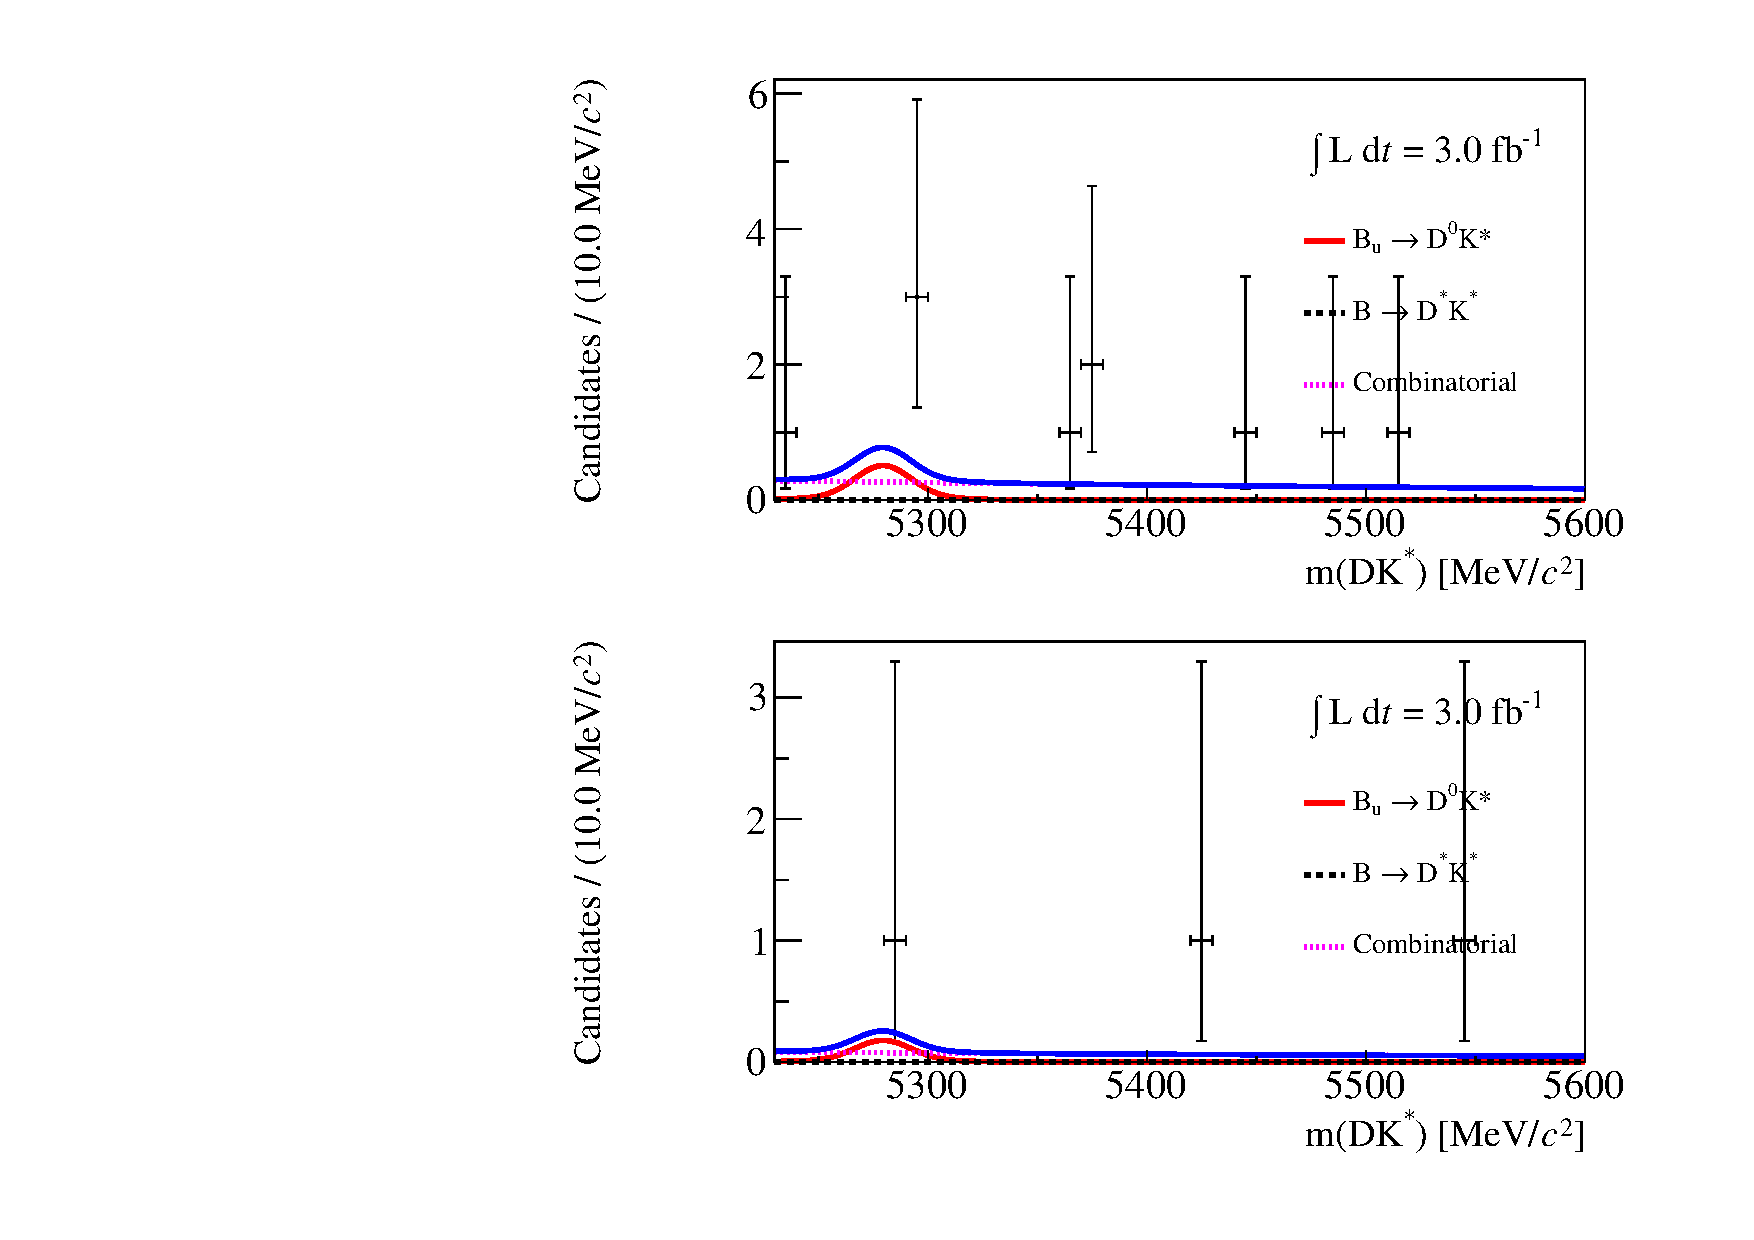
\includegraphics[width=0.3\linewidth]{figures/results/canvas_d2pikpipi_DD_run1.pdf}}
\caption{Results of the simultaneous fit for Run 1 data for 4-body modes. In each pair the top plot is for \Bp decays and the bottom plot is for \Bm decays.}
\label{datafit4bodyRun1}
\end{sidewaysfigure}

\begin{sidewaysfigure}[h]
\centering
\subfloat[$K\pi$, LL]{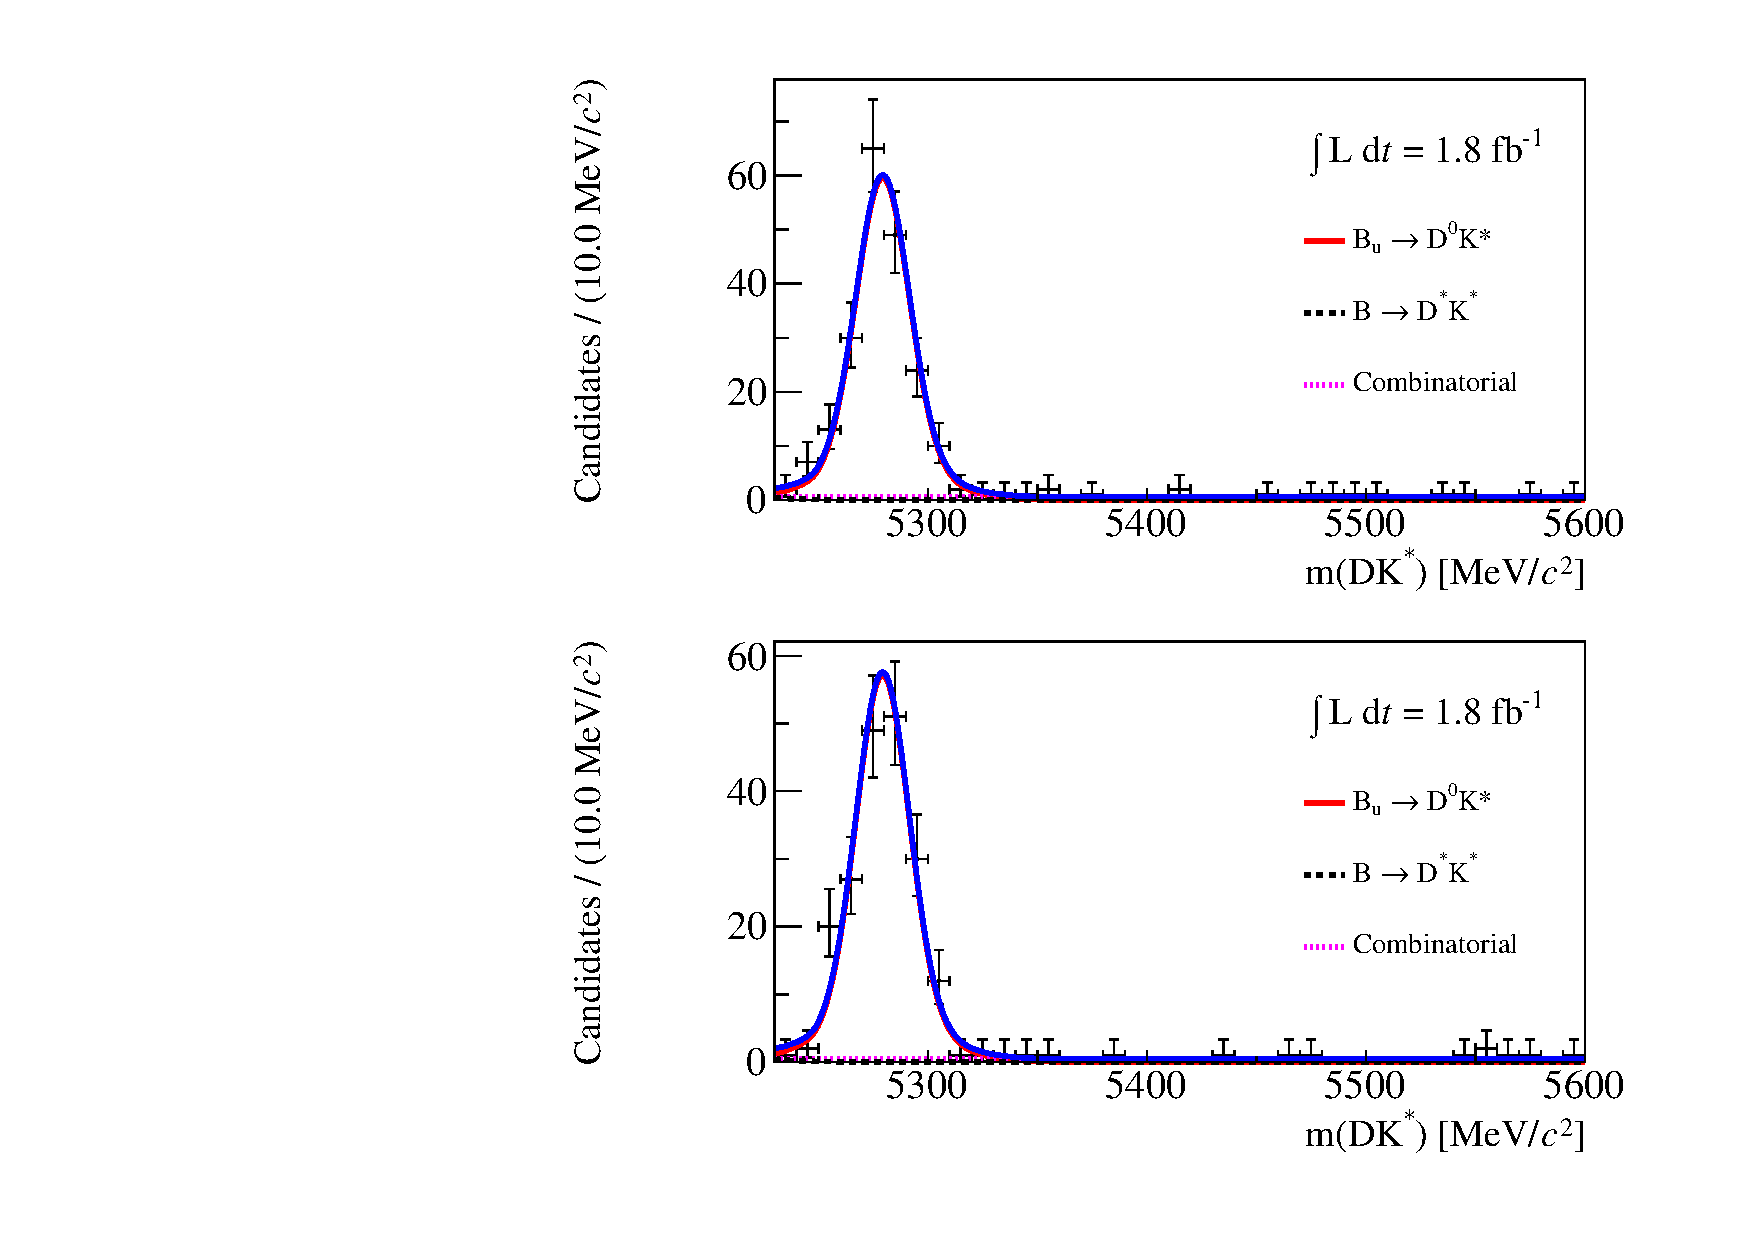
\includegraphics[width=0.25\linewidth]{figures/results/canvas_d2kpi_LL_run2.pdf}}
\hfill
\subfloat[$KK$, LL]{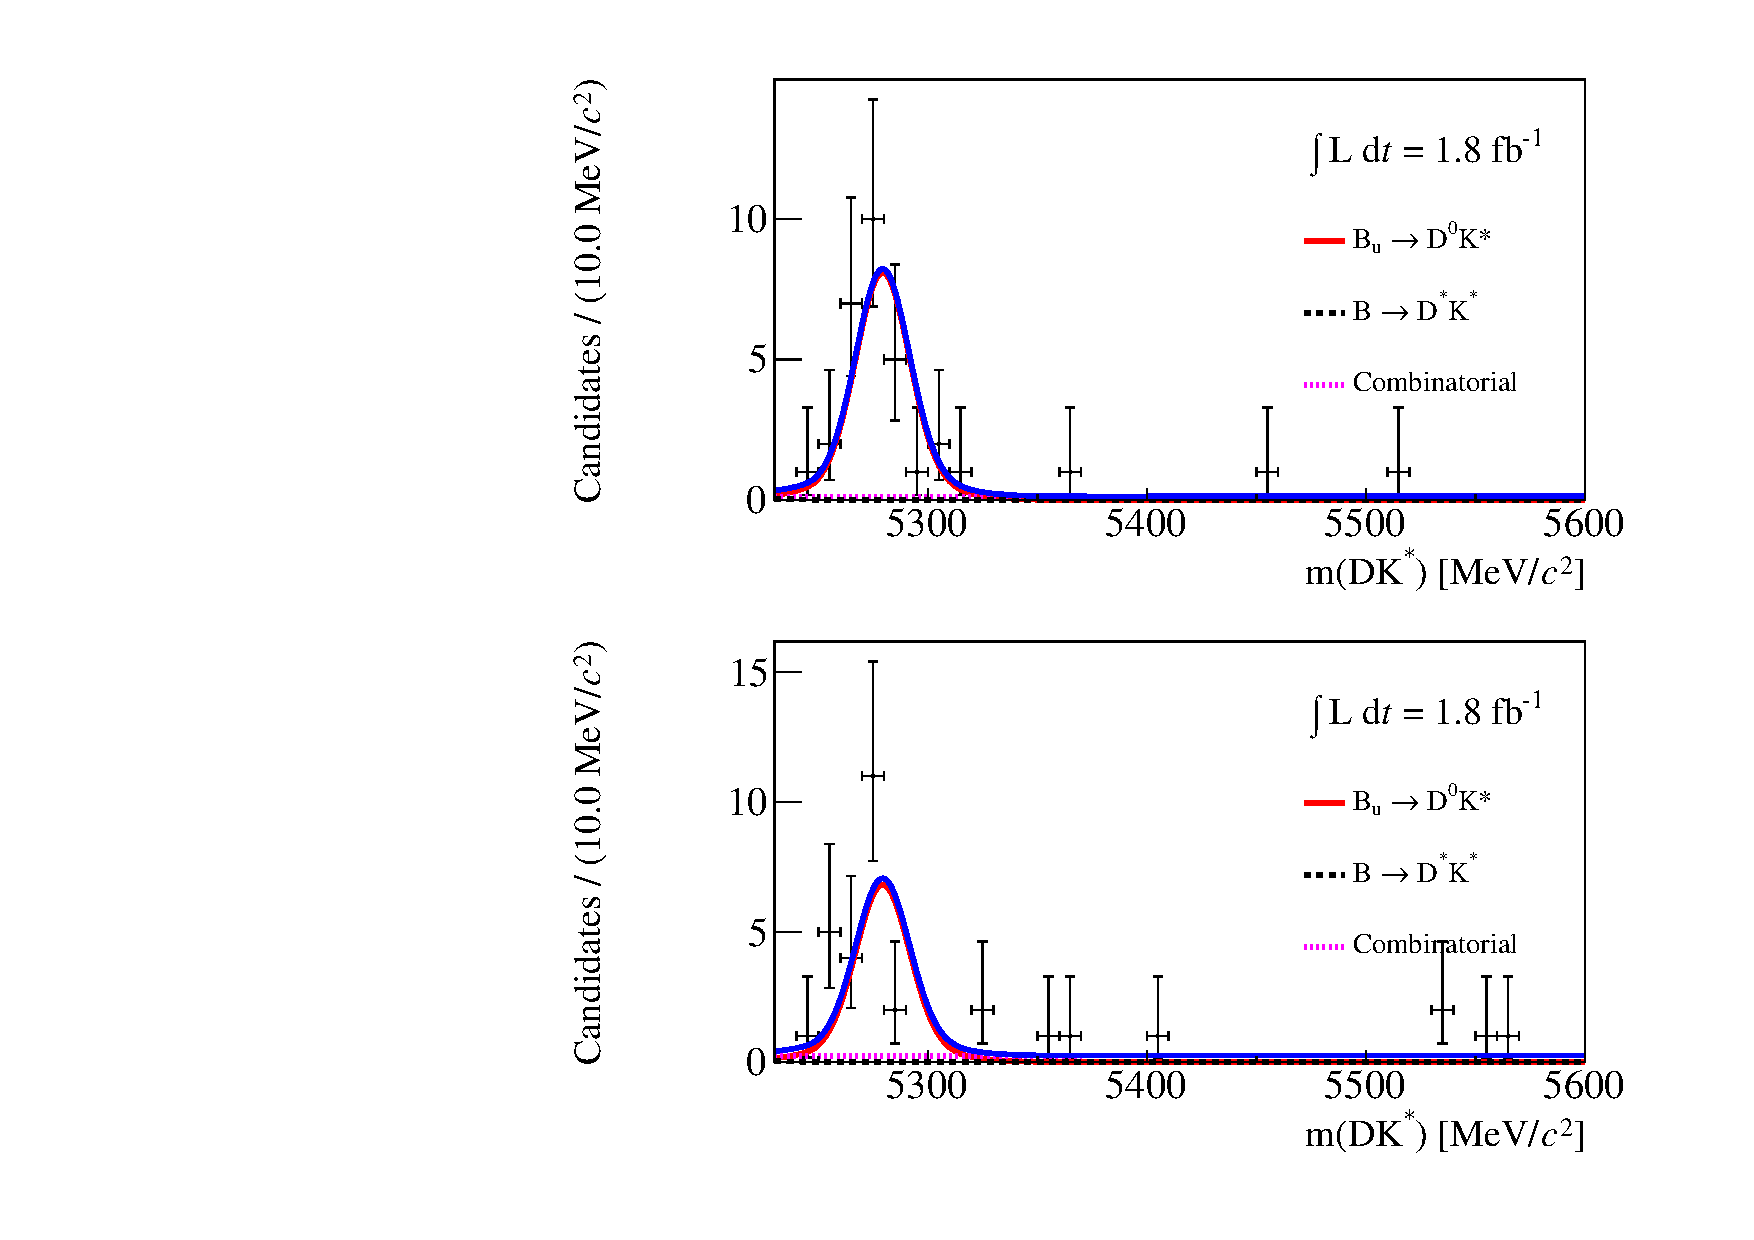
\includegraphics[width=0.25\linewidth]{figures/results/canvas_d2kk_LL_run2.pdf}}
\hfill
\subfloat[$\pi\pi$, LL]{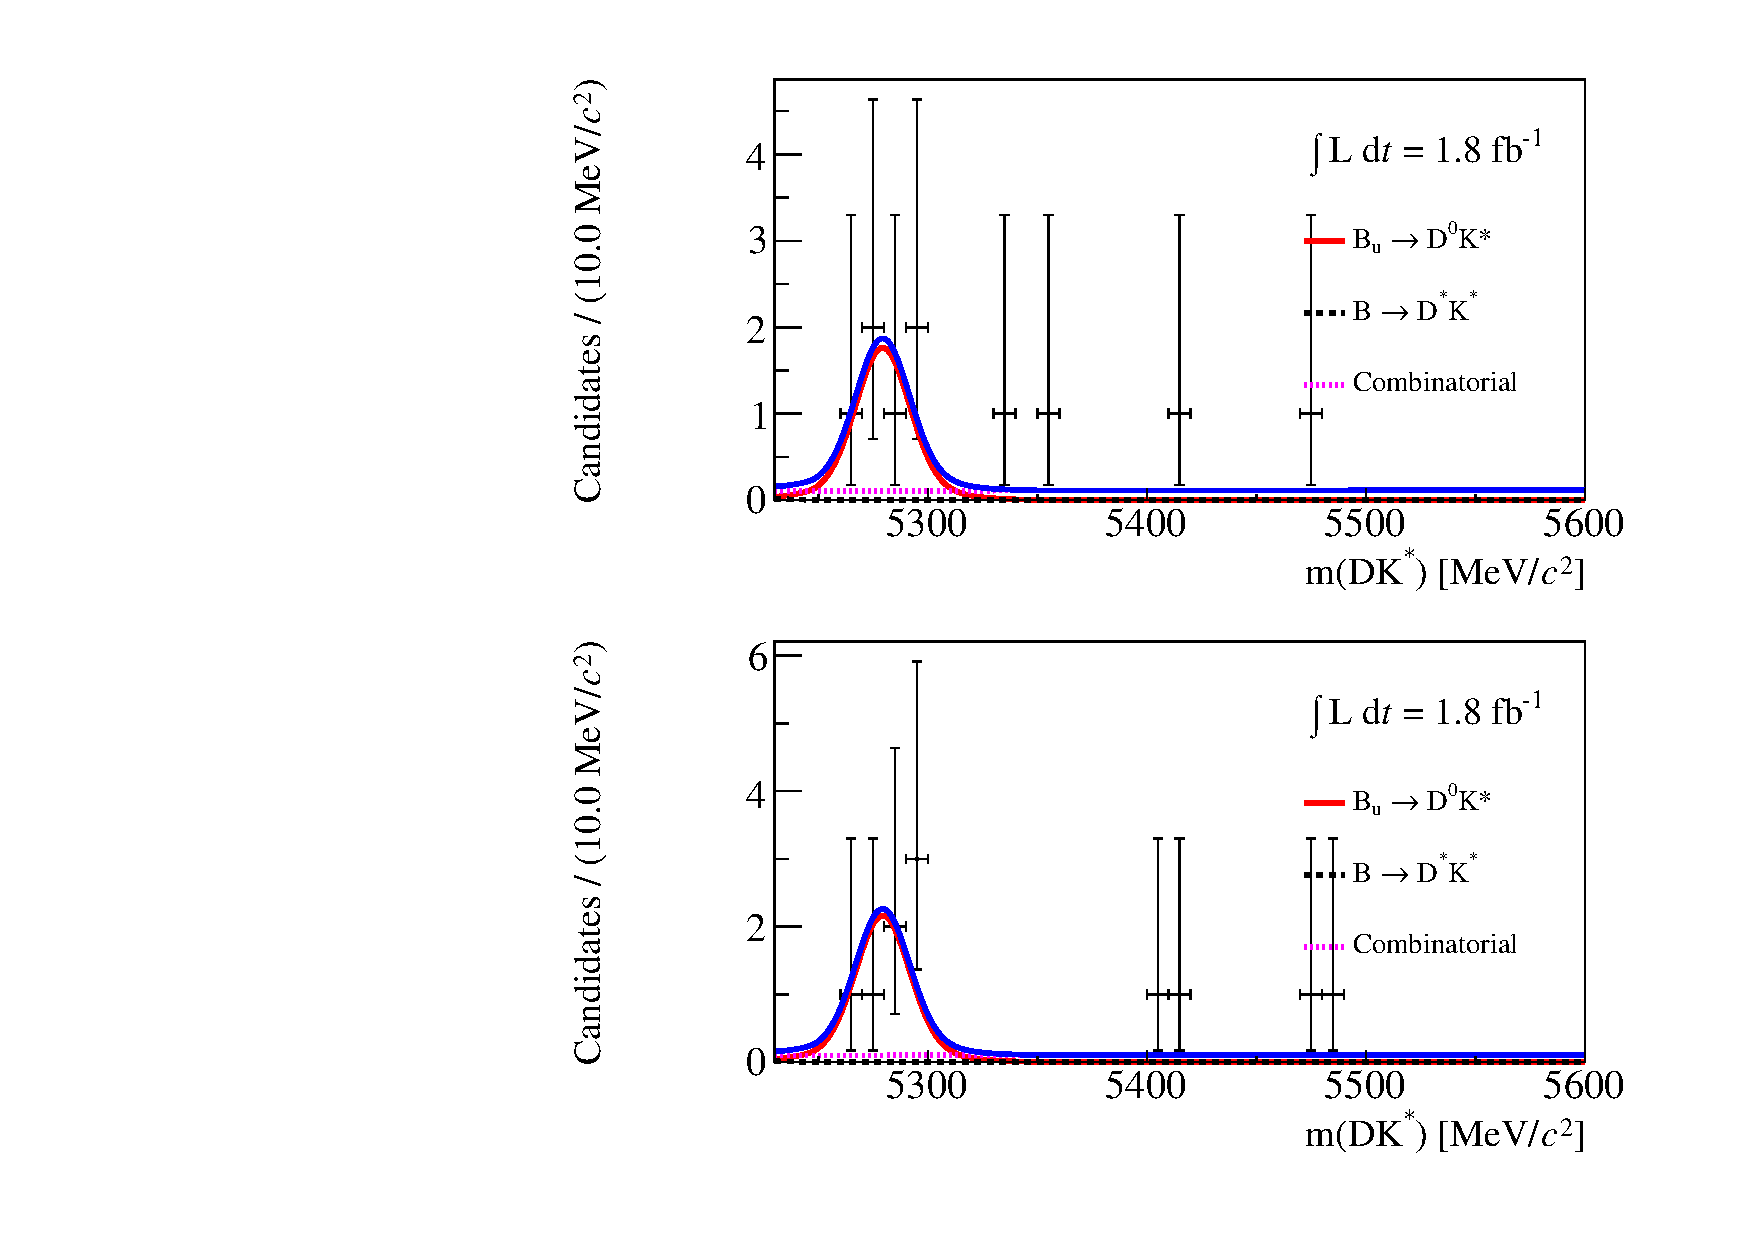
\includegraphics[width=0.25\linewidth]{figures/results/canvas_d2pipi_LL_run2.pdf}}
\hfill
\subfloat[$\pi K$, LL]{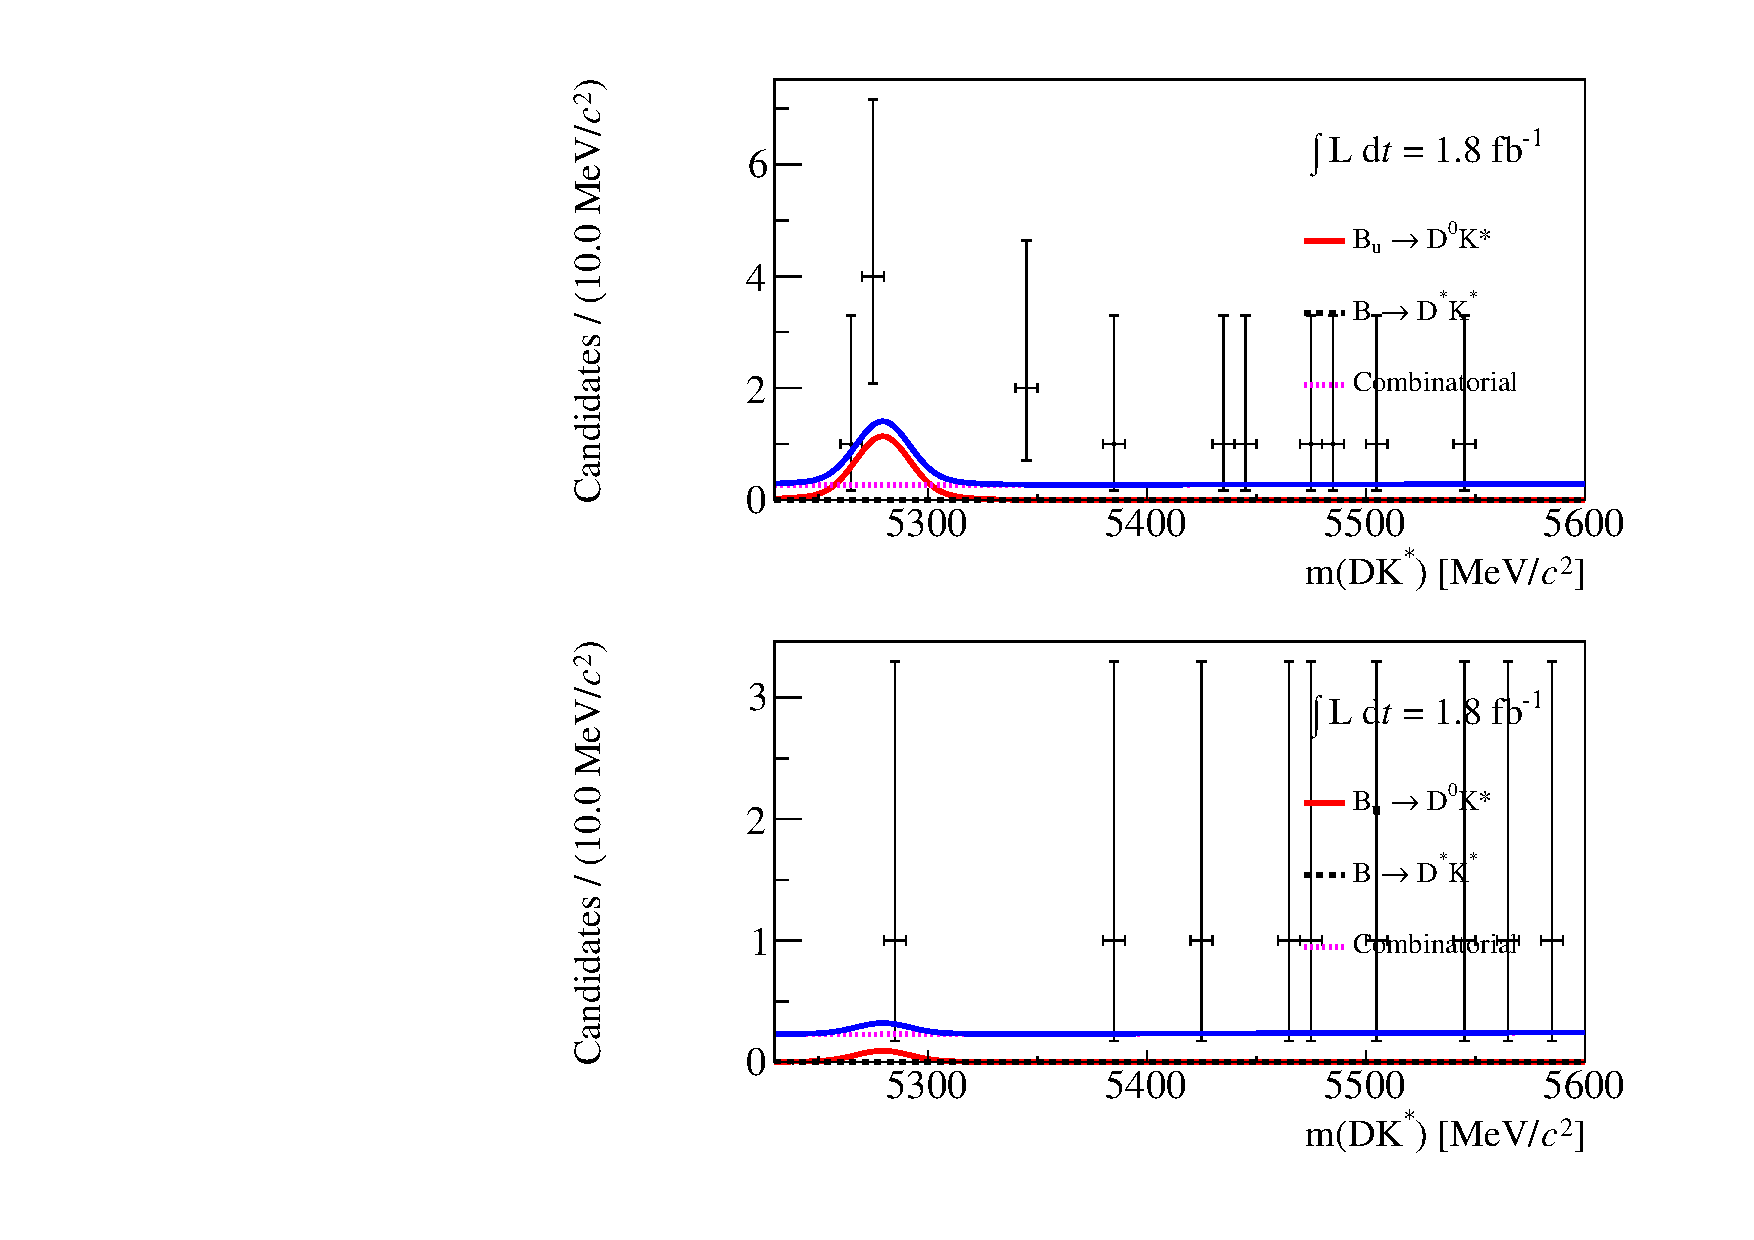
\includegraphics[width=0.25\linewidth]{figures/results/canvas_d2pik_LL_run2.pdf}}
\hfill
\subfloat[$K\pi$, DD]{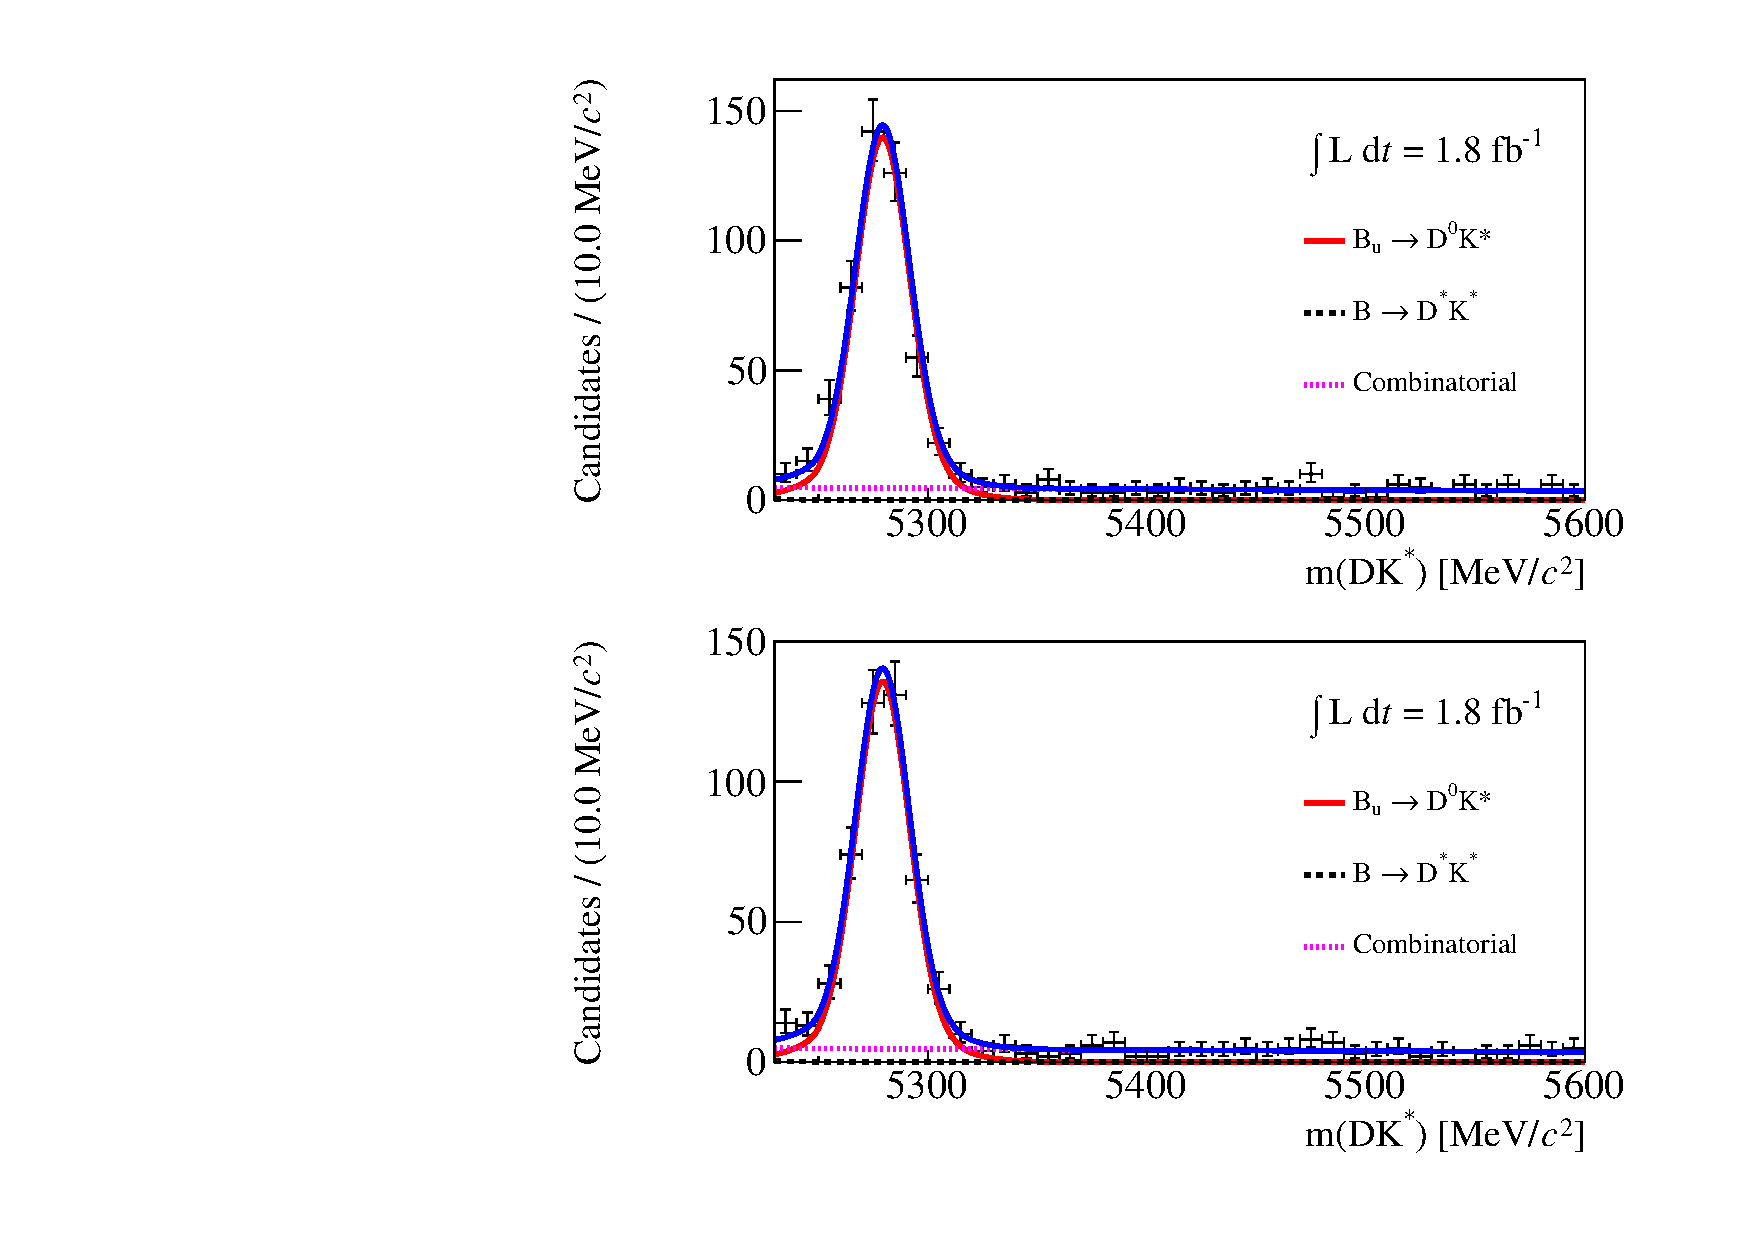
\includegraphics[width=0.25\linewidth]{figures/results/canvas_d2kpi_DD_run2.pdf}}
\hfill
\subfloat[$KK$, DD]{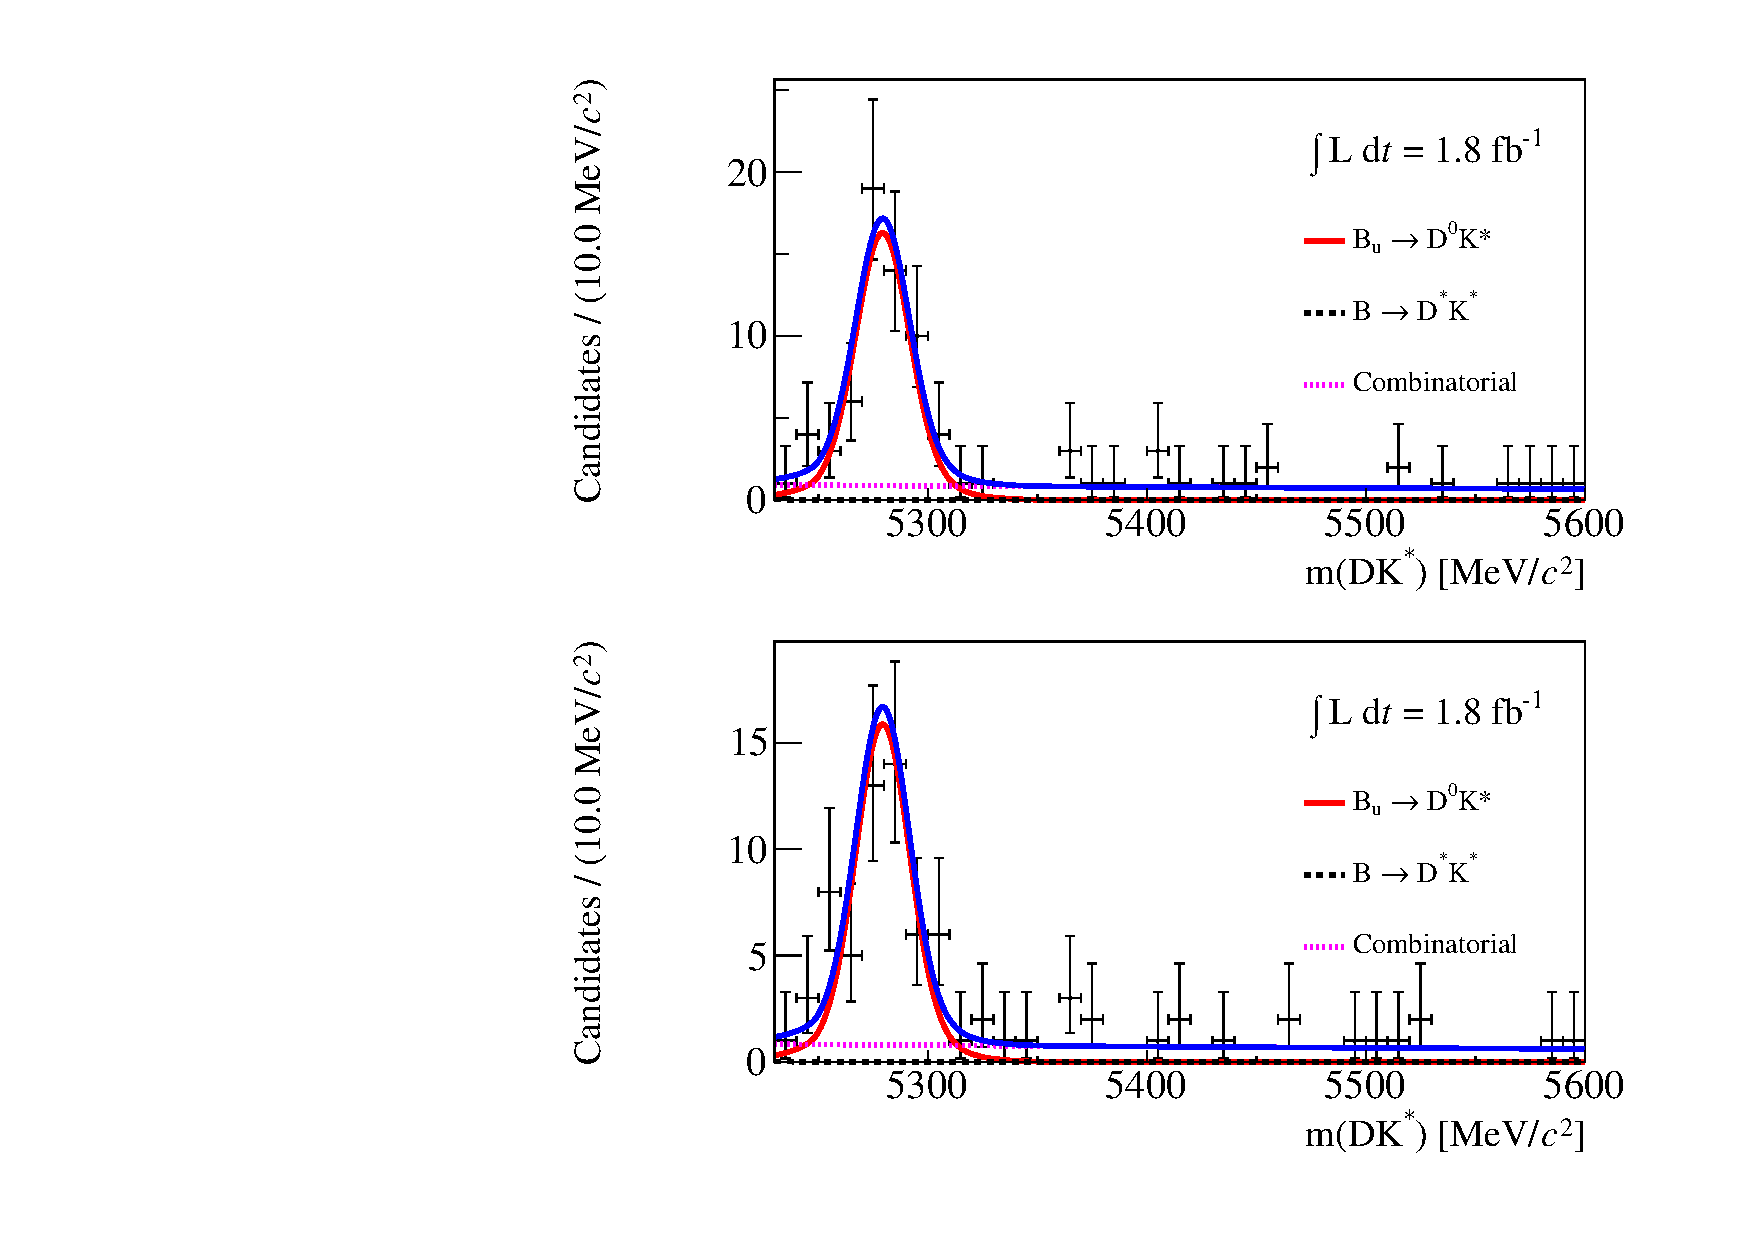
\includegraphics[width=0.25\linewidth]{figures/results/canvas_d2kk_DD_run2.pdf}}
\hfill
\subfloat[$\pi\pi$, DD]{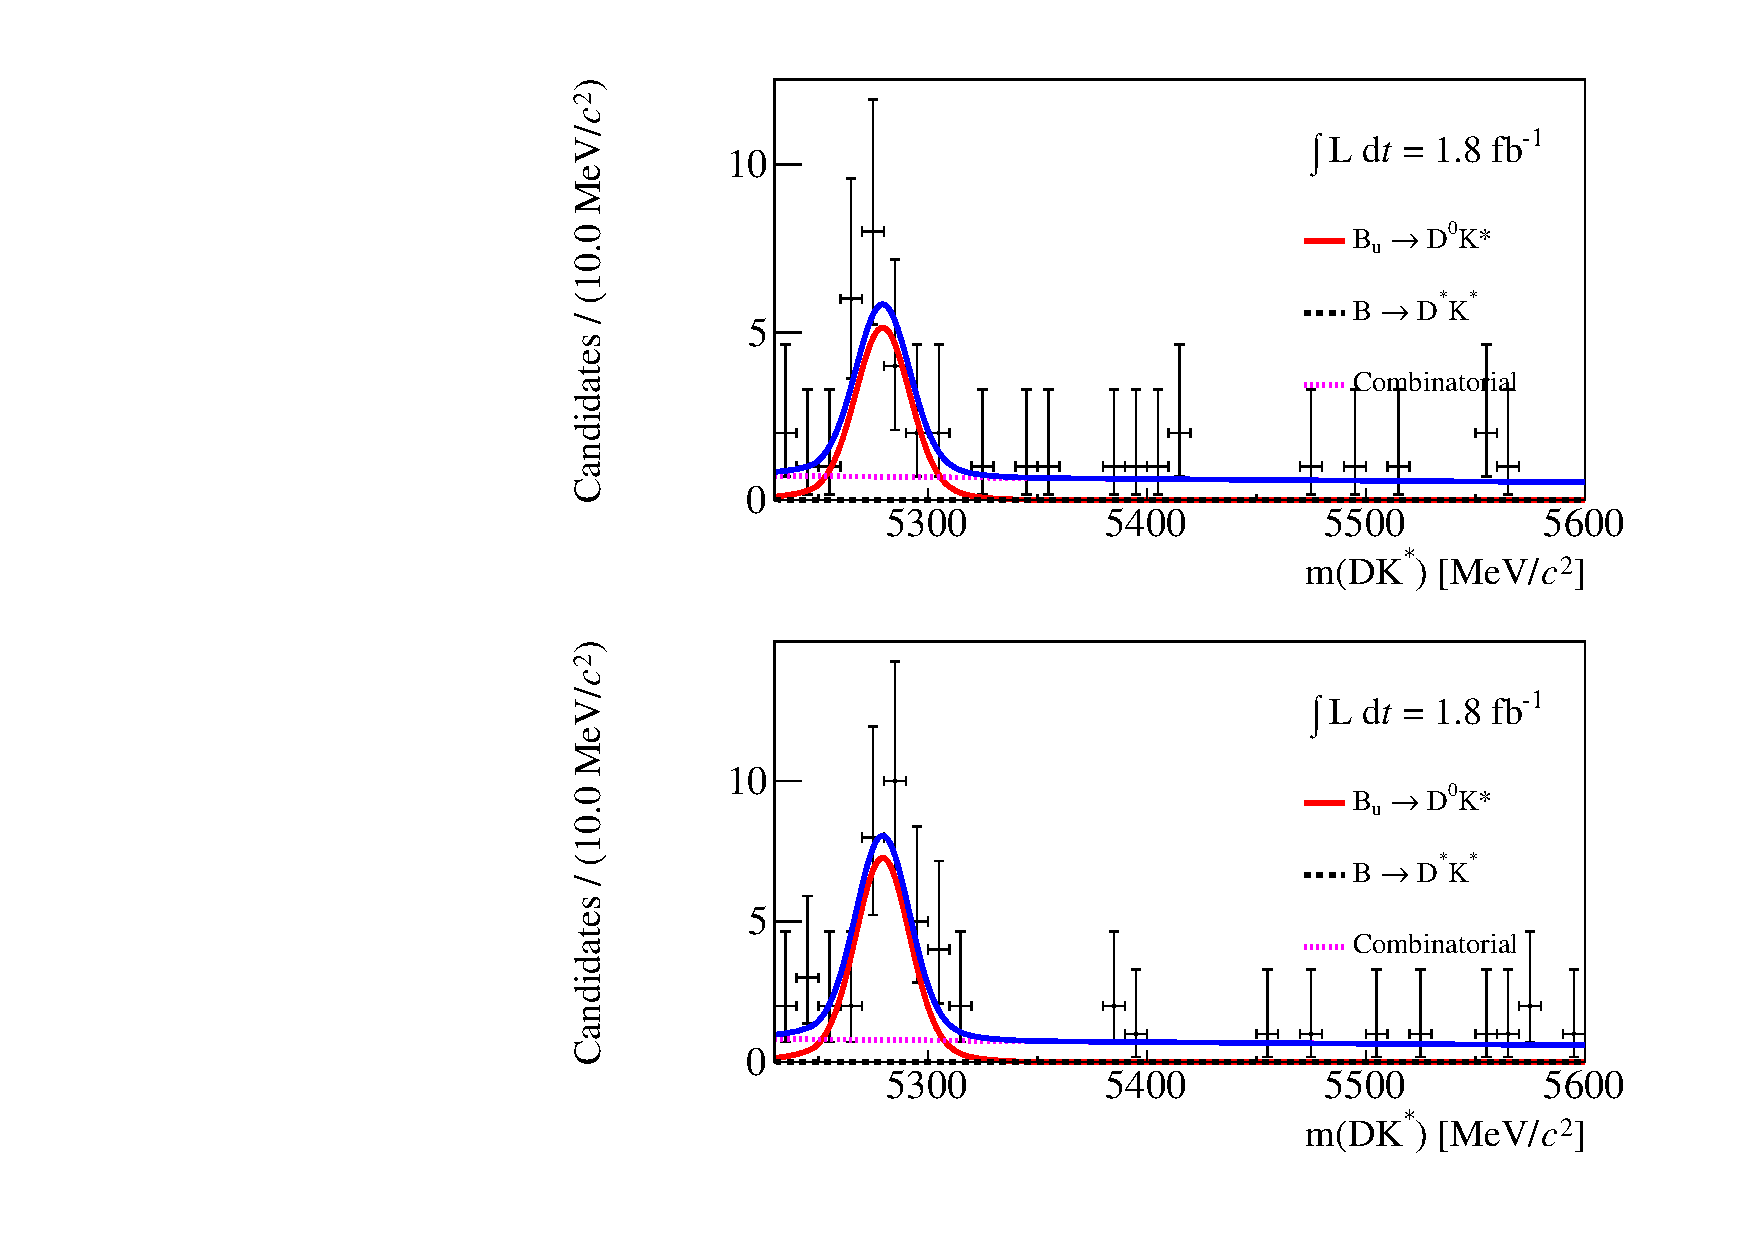
\includegraphics[width=0.25\linewidth]{figures/results/canvas_d2pipi_DD_run2.pdf}}
\hfill
\subfloat[$\pi K$, DD]{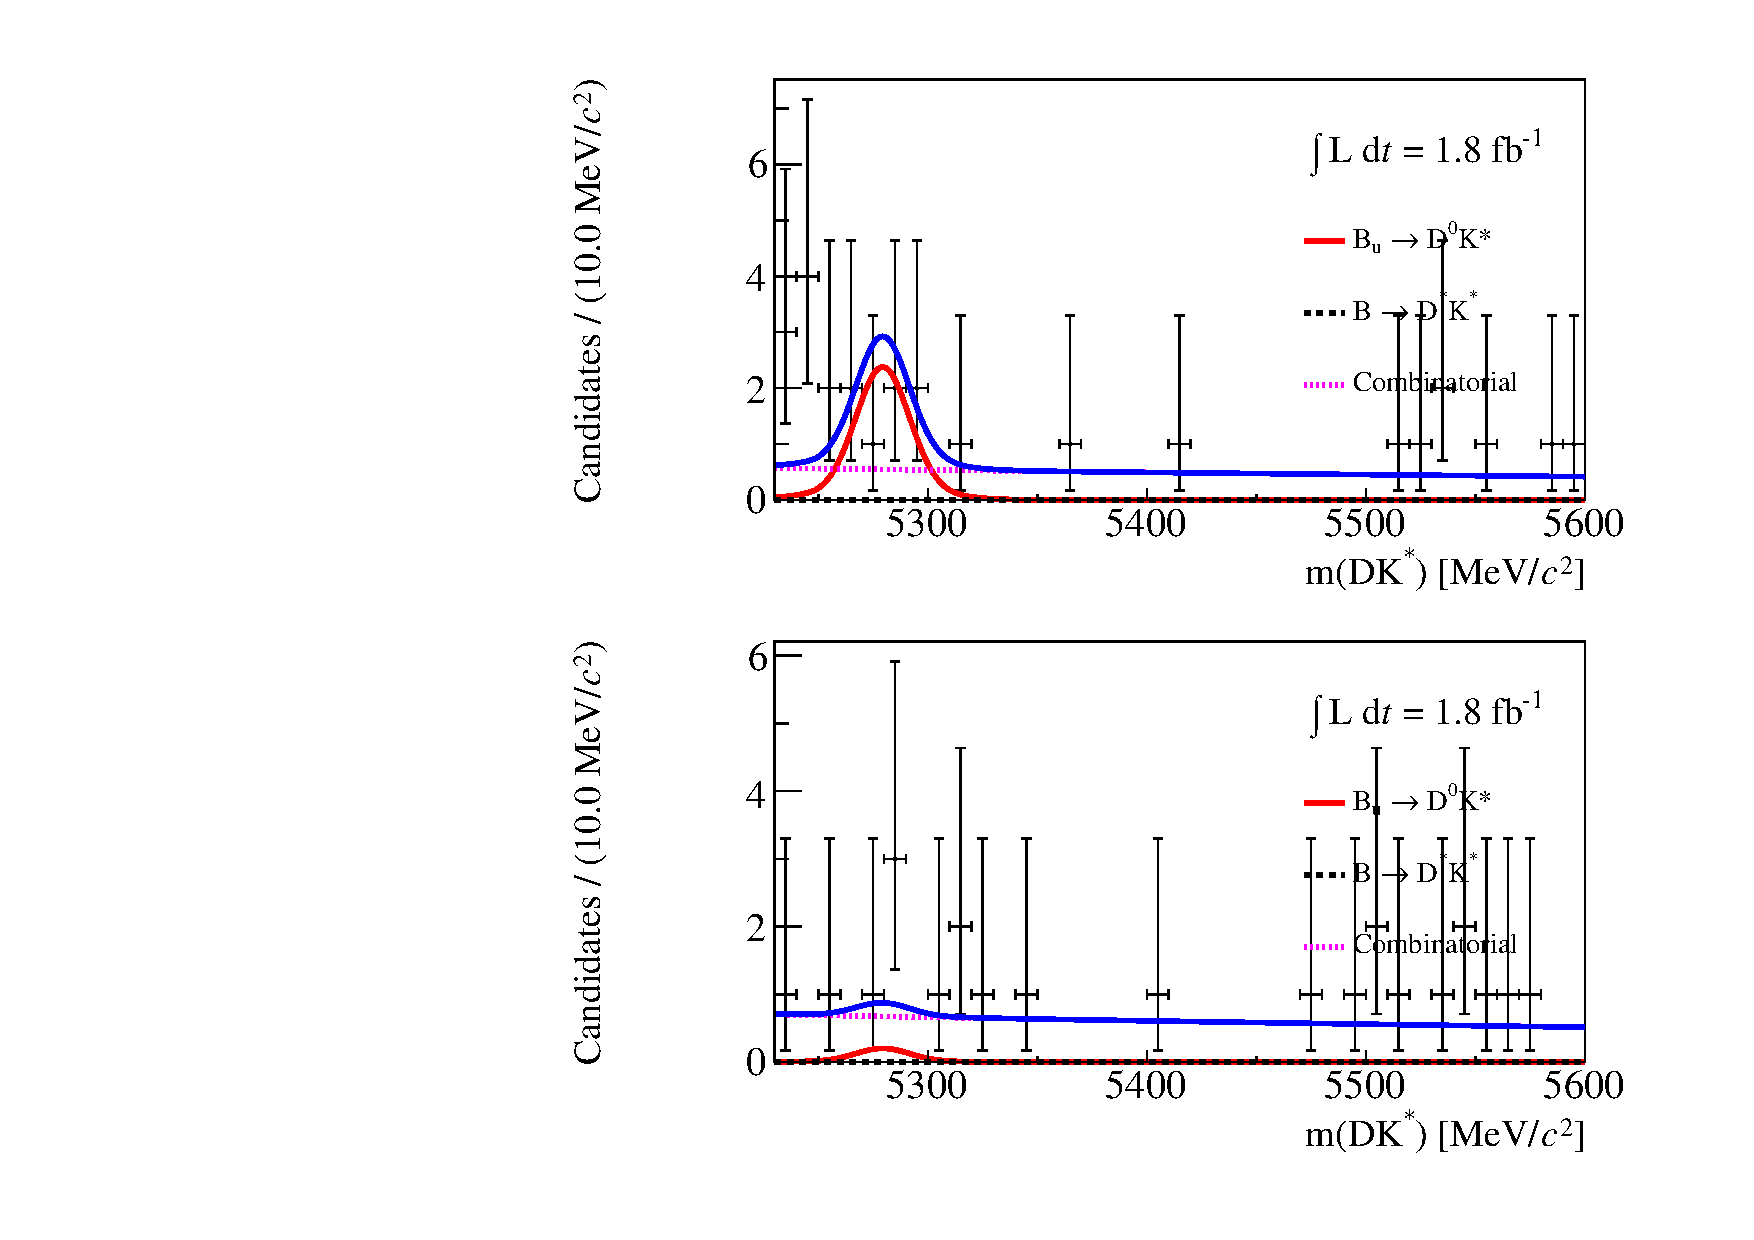
\includegraphics[width=0.25\linewidth]{figures/results/canvas_d2pik_DD_run2.pdf}}
\caption{Results of the simultaneous fit for Run 1 data for 2-body modes. In each pair the top plot is for \Bp decays and the bottom plot is for \Bm decays.}
\label{datafit2bodyRun2}
\end{sidewaysfigure}

\begin{sidewaysfigure}[h]
\centering
\subfloat[$K\pi\pi\pi$, LL]{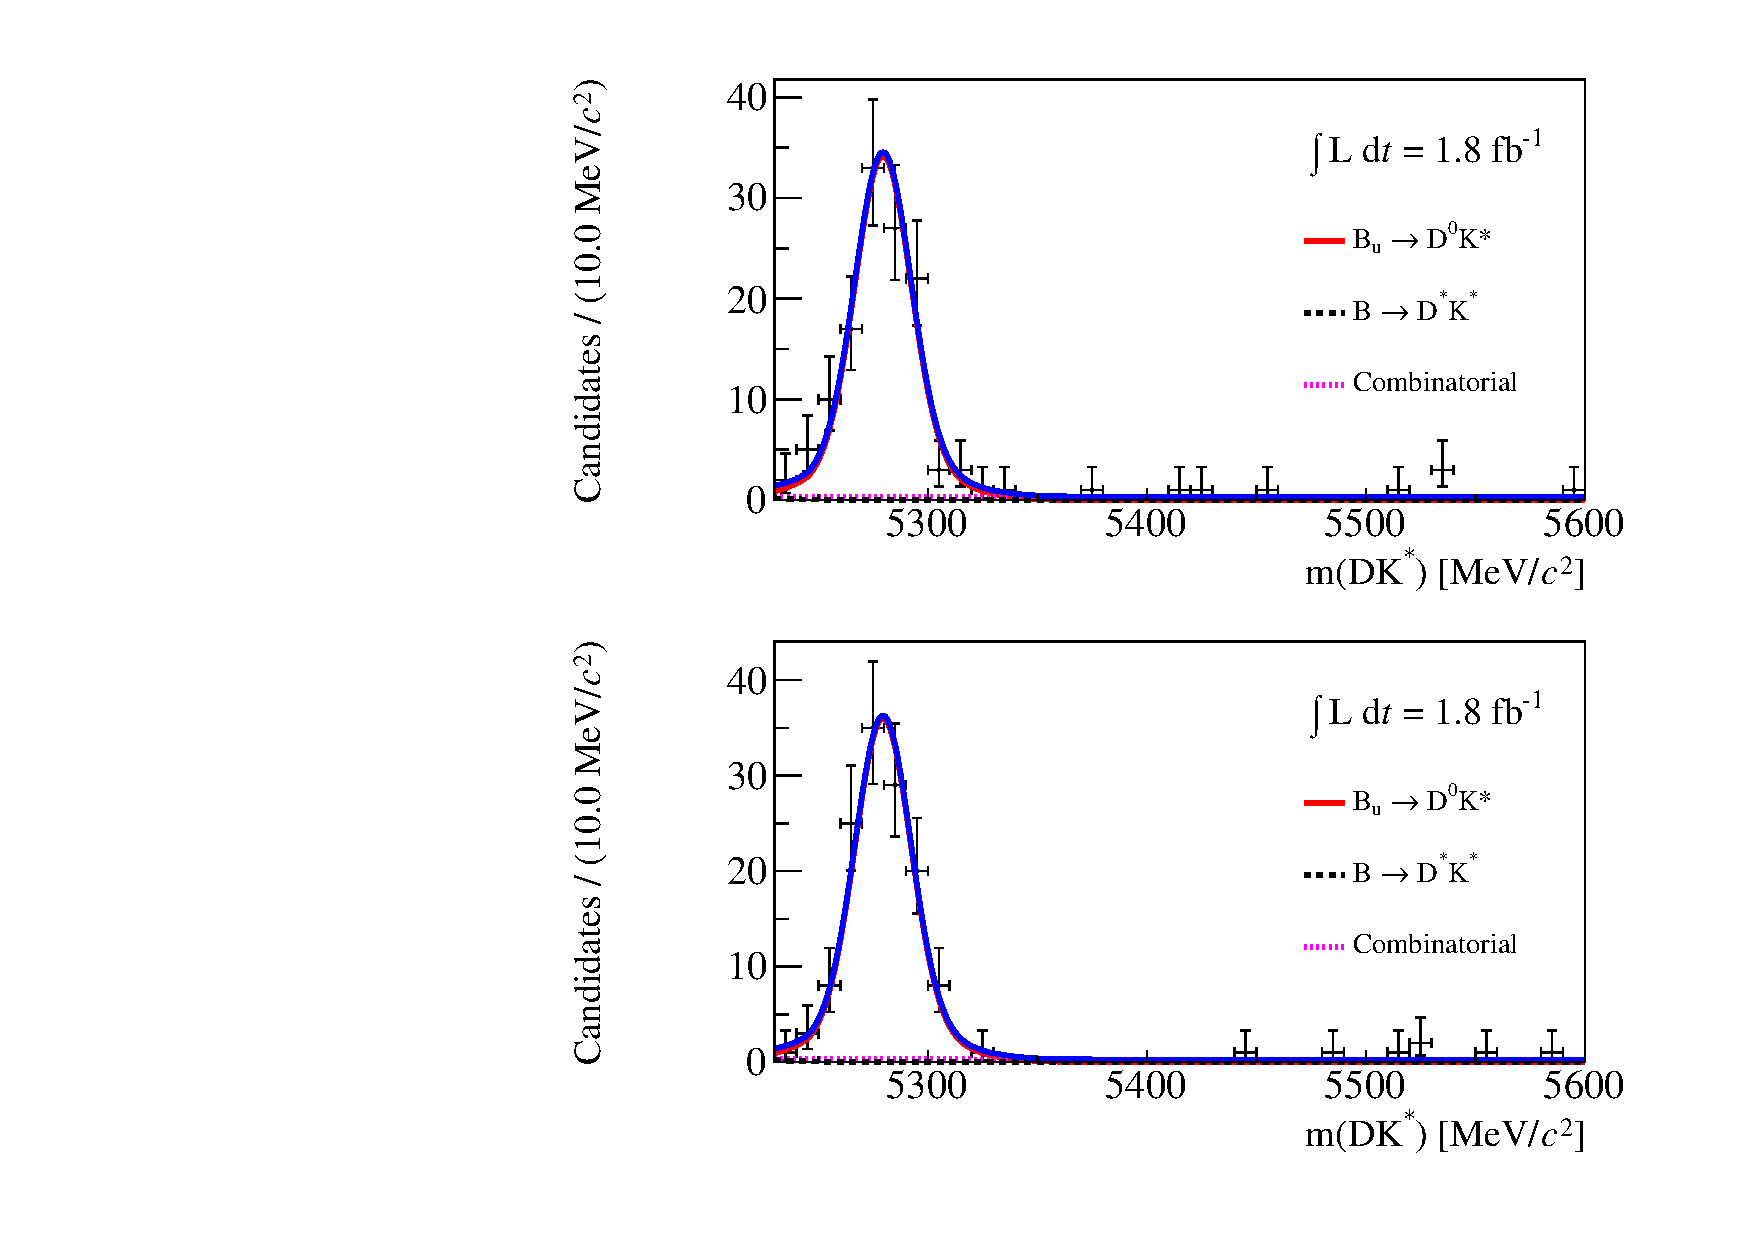
\includegraphics[width=0.3\linewidth]{figures/results/canvas_d2kpipipi_LL_run2.pdf}}
\hfill
\subfloat[$\pi\pi\pi\pi$, LL]{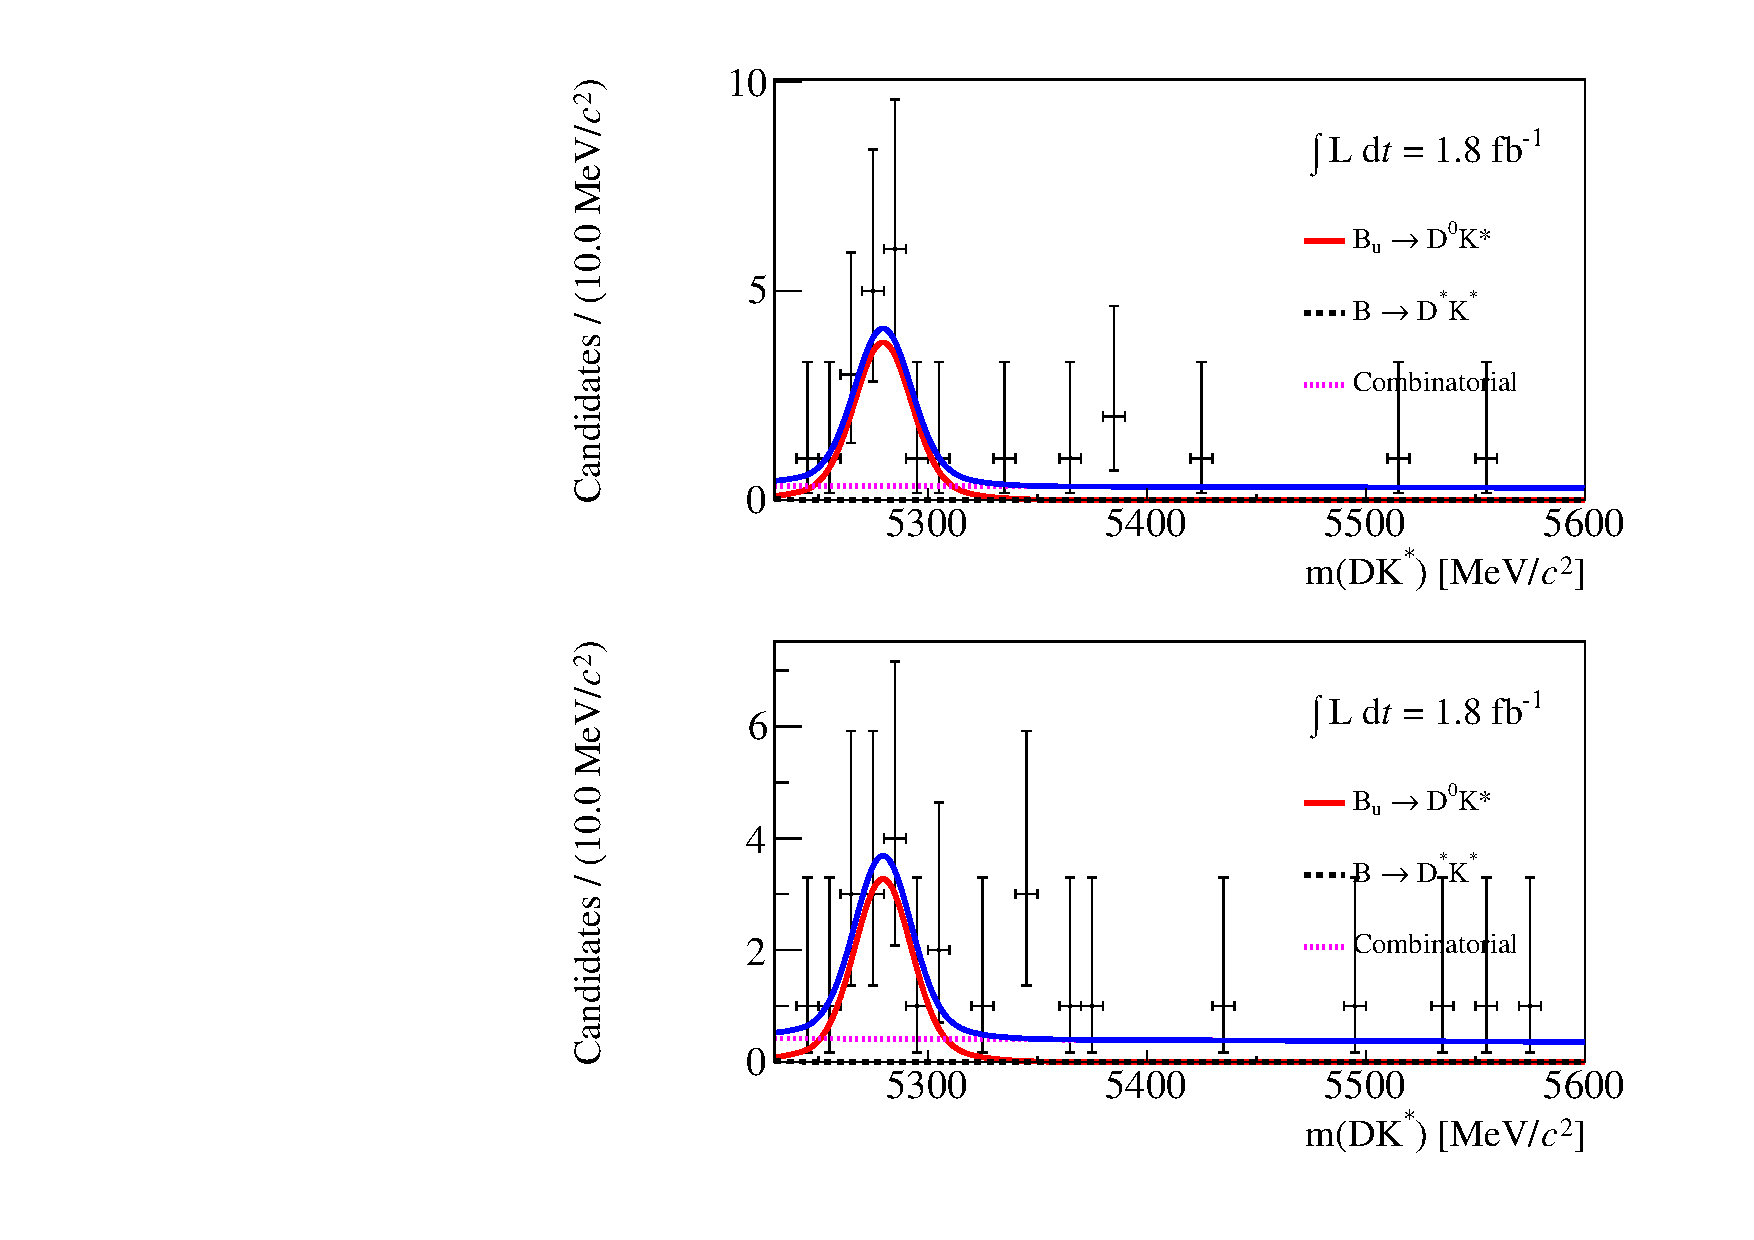
\includegraphics[width=0.3\linewidth]{figures/results/canvas_d2pipipipi_LL_run2.pdf}}
\hfill
\subfloat[$\pi K\pi\pi$, LL]{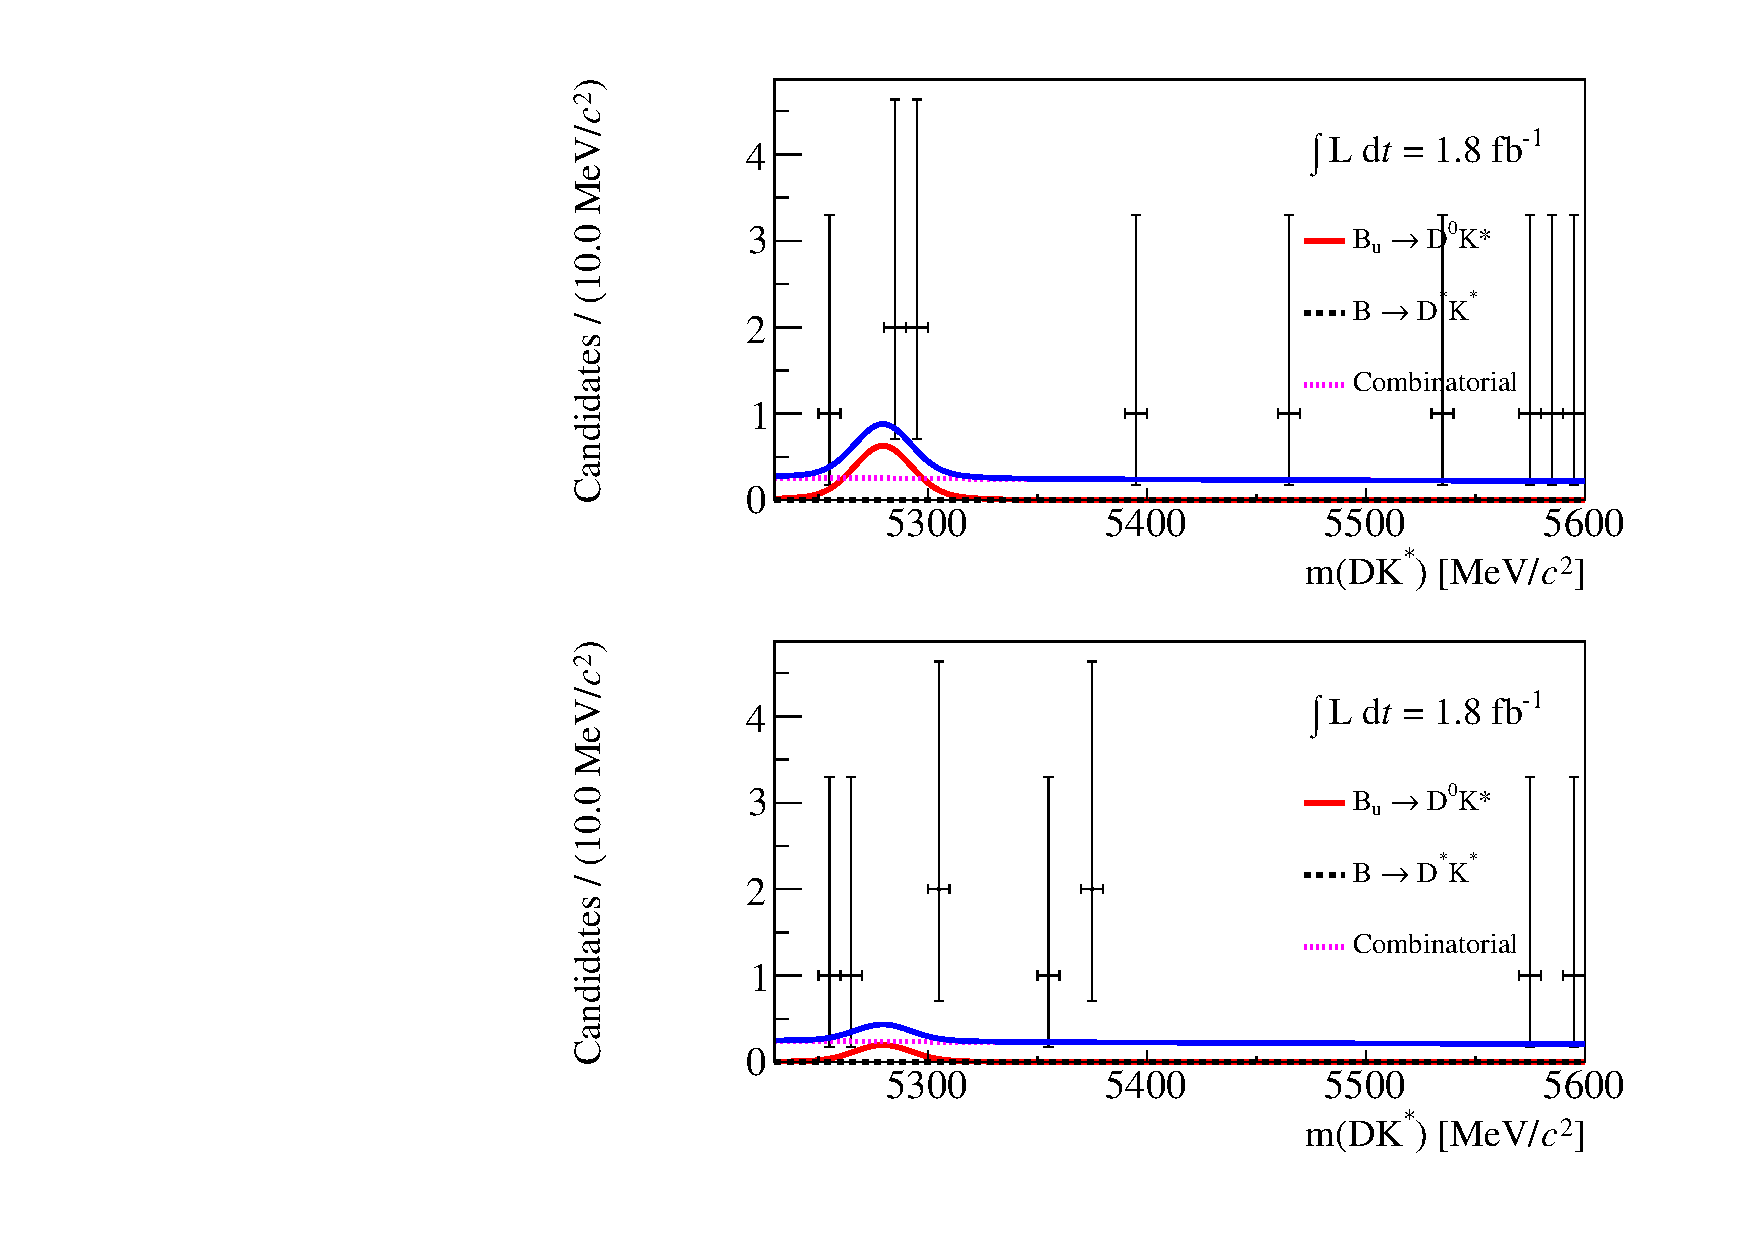
\includegraphics[width=0.3\linewidth]{figures/results/canvas_d2pikpipi_LL_run2.pdf}}
\hfill
\subfloat[$K\pi\pi\pi$, DD]{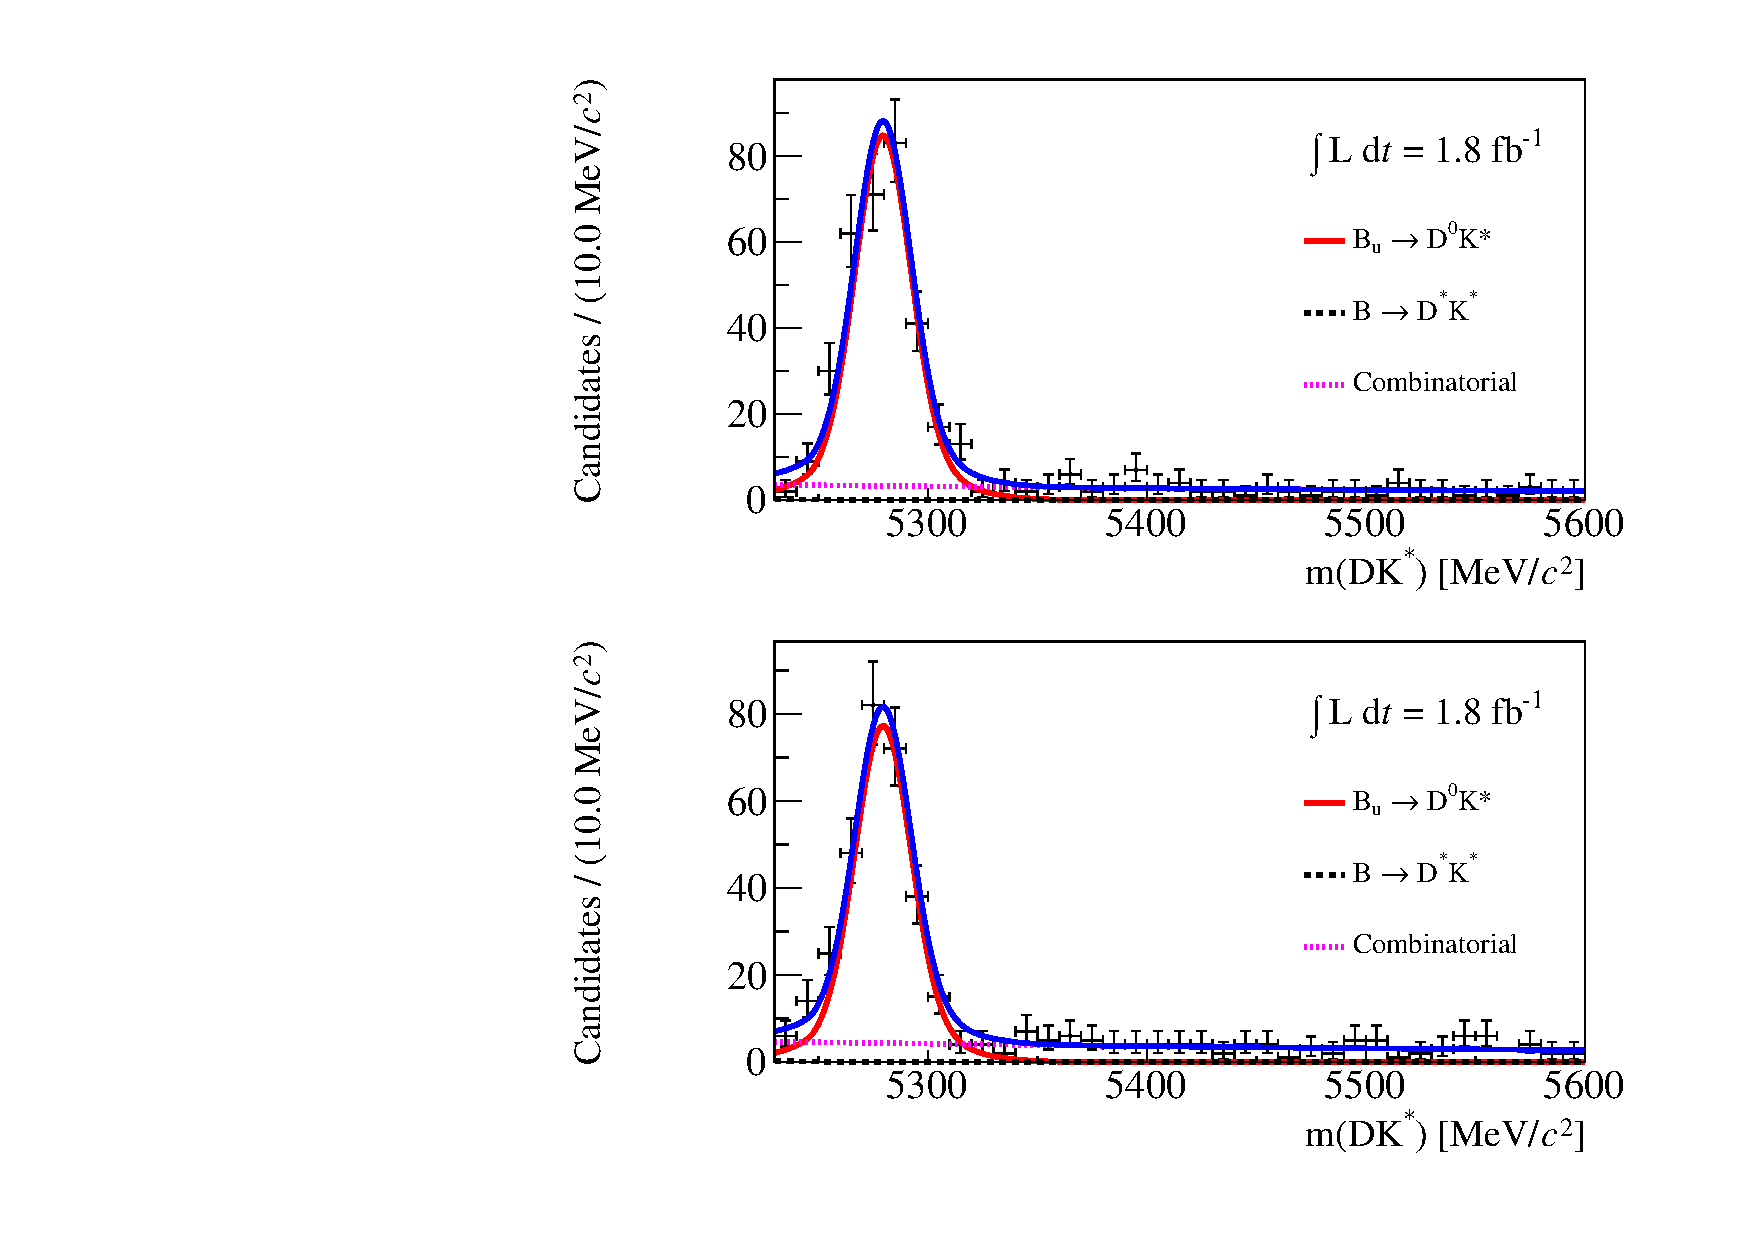
\includegraphics[width=0.3\linewidth]{figures/results/canvas_d2kpipipi_DD_run2.pdf}}
\hfill
\subfloat[$\pi\pi\pi\pi$, DD]{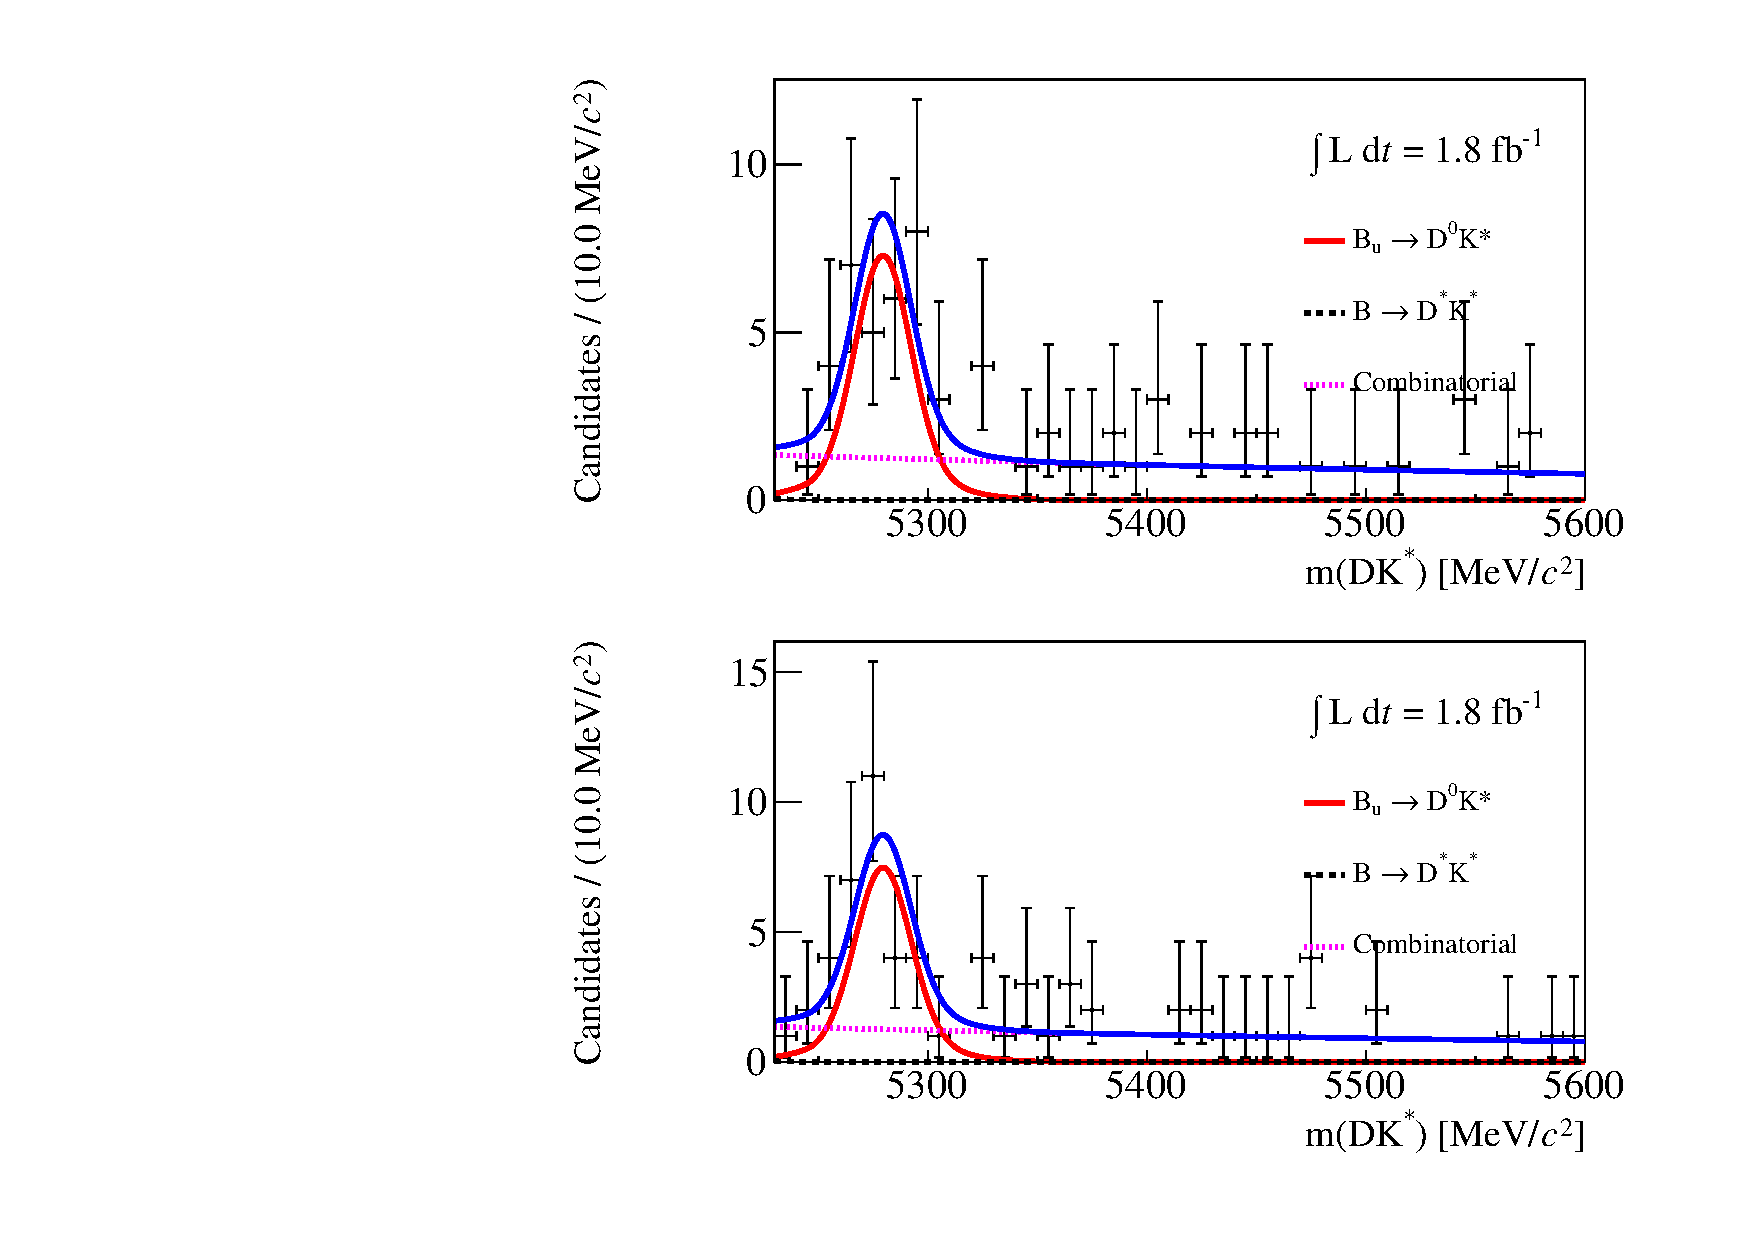
\includegraphics[width=0.3\linewidth]{figures/results/canvas_d2pipipipi_DD_run2.pdf}}
\hfill
\subfloat[$\pi K\pi\pi$, DD]{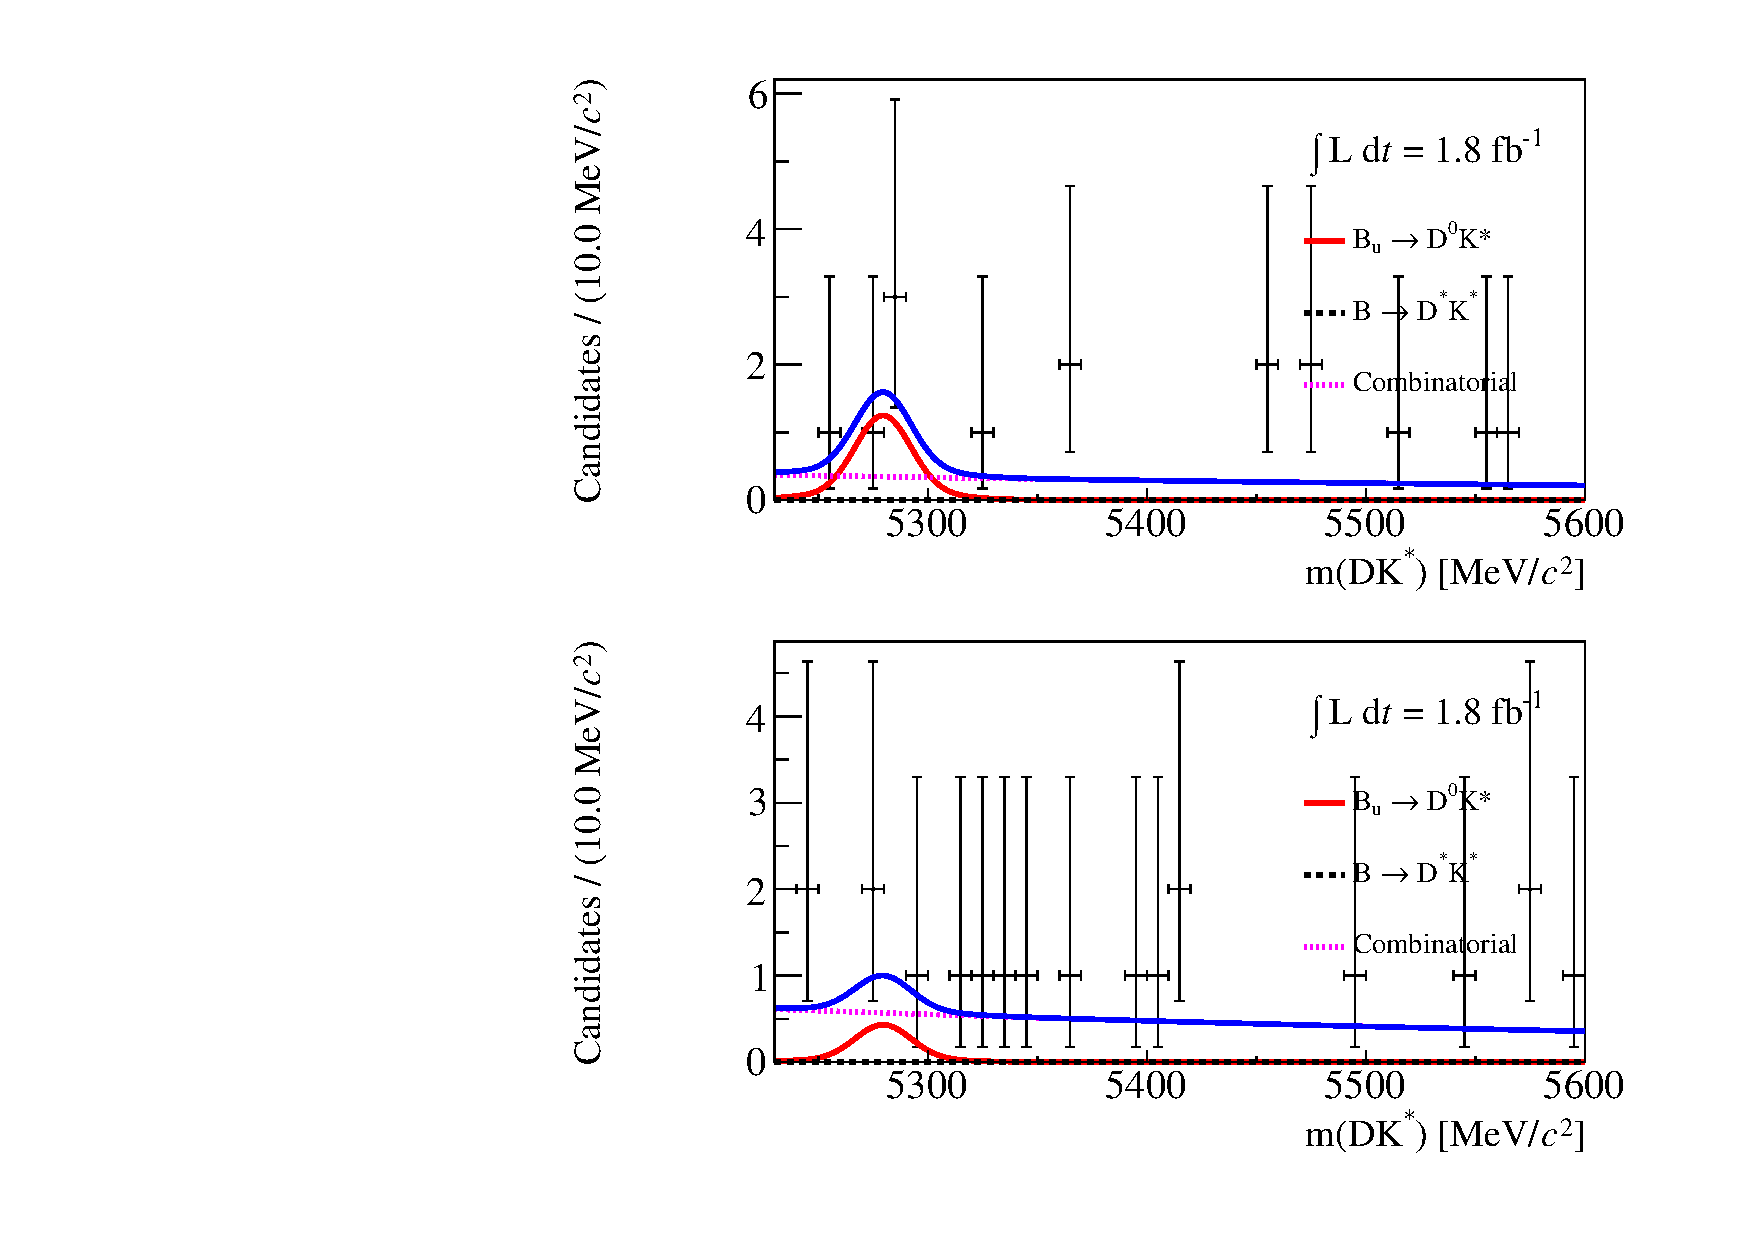
\includegraphics[width=0.3\linewidth]{figures/results/canvas_d2pikpipi_DD_run2.pdf}}
\caption{Results of the simultaneous fit for Run 1 data for 4-body modes. In each pair the top plot is for \Bp decays and the bottom plot is for \Bm decays.}
\label{datafit4bodyRun2}
\end{sidewaysfigure}

The statistical and systematic correlation matrices for the seven physics observables in the fit are shown in Tables \ref{statisticalcorrelations} and \ref{systematiccorrelations} respectively. Combined results from the $KK$ and $\pi\pi$ modes, taking correlations into account are,
\begin{align*}
R_{CP} = 1.20 \pm 0.08 \\
A_{CP} = 0.08 \pm 0.06
\end{align*}

Table \ref{cpfitresultsphysics} shows the fit results of the physics parameters of interest and Table \ref{cpfitresultsshapes} shows the fit results for $K\pi$ and $K\pi\pi\pi$ signal yields and shape parameters. All the combinatoric yields are left floating in the fit and these results are tabulated in Appendix \ref{sec:app:cpfit}.

\begin{table}[h]
\centering
{\footnotesize
\begin{tabular}{cccc}
Parameter & Fitted value & Negative error & Positive error \\
\hline
$A_{K\pi}$ & $-0.004$ & $-0.023$ & $0.023$ \\
$A_{KK}$ & $0.06$ & $-0.07$ & $0.07$ \\
$A_{\pi\pi}$ & $0.15$ & $-0.13$ & $0.13$ \\
$R_{KK}$ & $1.24$ & $-0.08$ & $0.09$ \\
$R_{\pi\pi}$ & $1.08$ & $-0.14$ & $0.15$ \\
$R^+_{K\pi}$ & $0.020$ & $-0.006$ & $0.006$ \\
$R^-_{K\pi}$ & $0.0018$ & $-0.0032$ & $0.0040$ \\
$A_{K\pi\pi\pi}$ & $-0.013$ & $-0.031$ & $0.031$ \\
$A_{\pi\pi\pi\pi}$ & $0.03$ & $-0.11$ & $0.11$ \\
$R_{\pi\pi\pi\pi}$ & $1.11$ & $-0.12$ & $0.13$ \\
$R^+_{K\pi\pi\pi}$ & $0.016$ & $-0.006$ & $0.008$ \\
$R^-_{K\pi\pi\pi}$ & $0.006$ & $-0.005$ & $0.006$ \\
\end{tabular}}
\caption{Fitted values of all the physics parameters from the \CP fit}
\label{cpfitresultsphysics}
\end{table}

\begin{table}[h]
\centering
{\footnotesize
\begin{tabular}{cccc}
Parameter & Fitted value & Negative error & Positive error \\
\hline
N\_d2kpi\_DD\_run1 & $503$ & $-22$ & $23$ \\
N\_d2kpi\_DD\_run2 & $911$ & $-32$ & $32$ \\
N\_d2kpi\_LL\_run1 & $228$ & $-14$ & $15$ \\
N\_d2kpi\_LL\_run2 & $388$ & $-19$ & $19$ \\
N\_d2kpipipi\_DD\_run1 & $233$ & $-15$ & $16$ \\
N\_d2kpipipi\_DD\_run2 & $560$ & $-26$ & $26$ \\
N\_d2kpipipi\_LL\_run1 & $101$ & $-9$ & $10$ \\
N\_d2kpipipi\_LL\_run2 & $251$ & $-16$ & $16$ \\
bu\_mean\_kpi & $5279.4$ & $-0.3$ & $0.3$ \\
bu\_mean\_kpipipi & $5279.5$ & $-0.5$ & $0.5$ \\
bu\_width\_kpi & $12.1$ & $-0.3$ & $0.3$ \\
bu\_width\_kpipipi & $12.6$ & $-0.4$ & $0.4$ \\
exp\_kpi\_DD\_combs\_slope & $-0.0008$ & $-0.0006$ & $0.0006$ \\
exp\_kpi\_LL\_combs\_slope & $0.0002$ & $-0.0011$ & $0.0012$ \\
exp\_kpipipi\_DD\_combs\_slope & $-0.0014$ & $-0.0006$ & $0.0006$ \\
exp\_kpipipi\_LL\_combs\_slope & $-0.0003$ & $-0.0014$ & $0.0015$ \\
\end{tabular}}
\caption{Fitted values of the signal yields and shape parameters from the \CP fit}
\label{cpfitresultsshapes}
\end{table}

\begin{sidewaystable}[h]
\centering
{\footnotesize
\begin{tabular}{c|cccccccccccc} 
\hline 
& $A_{K\pi}$ & $A_{KK}$ & $A_{\pi\pi}$ & $R_{KK}$ & $R_{\pi\pi}$ & $R^+_{K\pi}$ & $R^-_{K\pi}$ & $A_{K\pi\pi\pi}$ & $A_{\pi\pi\pi\pi}$ & $R_{\pi\pi\pi\pi}$ & $R^+_{K\pi\pi\pi}$ & $R^-_{K\pi\pi\pi}$ \\ 
 \hline
$A_{K\pi}$ & 1 & 0.00020  & 0.00017  & -0.00005  & -0.0006  & 0.076  & -0.014  & 0.0000027  & -0.000021  & 0.0011  & -0.0000045  & 0.0000028  \\
$A_{KK}$ & & 1  & -0.00012  & -0.0030  & -0.000038  & -0.0011  & -0.0024  & 0.0000054  & -0.00012  & 0.000085  & 0.000004  & 0.0000032  \\
$A_{\pi\pi}$ &  &  & 1  & -0.00062  & -0.022  & -0.0019  & -0.0017  & -0.0000021  & 0.000062  & 0.0010  & 0.000016  & 0.000017  \\
$R_{KK}$ & & & & 1  & 0.064  & 0.034  & 0.014  & -0.0000029  & 0.000057  & 0.065  & 0.000087  & 0.00011  \\
$R_{\pi\pi}$ & & & & & 1  & 0.027  & 0.017  & 0.000034  & -0.00013  & 0.030  & -0.00011  & -0.000056  \\
$R^+_{K\pi}$ & & & & & & 1  & 0.020  & 0.000016  & 0.0000014  & 0.0095  & -0.000044  & -0.000033 \\
$R^-_{K\pi}$ & & & & & & & 1  & 0.000010  & 0.00018  & -0.0050  & 0.0000095  & 0.000034  \\
$A_{K\pi\pi\pi}$ & & & & & & & & 1  & -0.00048  & -0.0014  & 0.067  & -0.033  \\
$A_{\pi\pi\pi\pi}$ & & & & & & & & & 1  & 0.00085  & 0.0029  & 0.0034  \\
$R_{\pi\pi\pi\pi}$ & & & & & & & & & & 1  & 0.031  & 0.039  \\
$R^+_{K\pi\pi\pi}$ & & & & & & & & & & & 1  & 0.028  \\
$R^-_{K\pi\pi\pi}$ & & & & & & & & & & & & 1  \\
\hline 
\end{tabular}}
\caption{Statistical correlation matrix for the seven physics observables from the \CP fit to data. The matrix is symmetric so only the top half is shown.}
\label{statisticalcorrelations}
\end{sidewaystable}
\begin{sidewaystable}[h]
\centering
{\footnotesize
\begin{tabular}{c|cccccccccccc} 
\hline 
& $A_{K\pi}$ & $A_{KK}$ & $A_{\pi\pi}$ & $R_{KK}$ & $R_{\pi\pi}$ & $R^+_{K\pi}$ & $R^-_{K\pi}$ & $A_{K\pi\pi\pi}$ & $A_{\pi\pi\pi\pi}$ & $R_{\pi\pi\pi\pi}$ & $R^+_{K3\pi}$ & $R^-_{K3\pi}$ \\ 
 \hline
$A_{K\pi}$ & 1 & 0.83  & -0.0067  & 0.72  & -0.0035  & 0.0071  & -0.025  & 0.94  & 0.84  & 0.00071  & -0.011  & -0.003  \\
$A_{KK}$ &  & 1  & -0.028  & 0.65  & 0.014  & 0.014  & -0.021  & 0.83  & 0.77  & 0.0034  & -0.0029  & 0.0045  \\
$A_{\pi\pi}$ &  &  & 1  & 0.0061  & 0.014  & 0.03  & 0.016  & -0.0073  & 0.0031  & -0.019  & -0.0056  & -0.0094  \\
$R_{KK}$ & & & & 1  & -0.032  & -0.0054  & -0.02  & 0.72  & 0.68  & -0.0028  & -0.00051  & 0.011  \\
$R_{\pi\pi}$ & & & &  & 1  & 0.057  & 0.079  & -0.0092  & 0.0012  & -0.01  & -0.017  & 0.0097  \\
$R^+_{K\pi}$ & & & & &  & 1  & 0.079  & -0.0082  & 0.0037  & -0.0022  & -0.0098  & -0.0099  \\
$R^-_{K\pi}$ & & & & & &  & 1  & -0.013  & -0.0063  & -0.012  & 0.0067  & 0.03  \\
$A_{K\pi\pi\pi}$ & & & & & & &   & 1  & 0.84  & -0.005  & -0.01  & -0.015  \\
$A_{\pi\pi\pi\pi}$ & & & & & & & &   & 1  & 0.036  & 0.0053  & 0.00047  \\
$R_{\pi\pi\pi\pi}$ & & & & & & & & &   & 1  & 0.0089  & -0.0086  \\
$R^-_{K3\pi}$ & & & & & & & & & &   & 1  & 0.045  \\
$R^-_{K3\pi}$ & & & & & & & & & & &   & 1  \\
\hline 
\end{tabular}}
\caption{Systematic correlation matrix for the seven physics observables from the \CP fit to data. The matrix is symmetric so only the top half is shown.}
\label{systematiccorrelations}
\end{sidewaystable}

The fitted yields obtained for running the fit with \Bp and \Bm samples combined are given in Table \ref{fittedyields}. 
%The simultaneous fit was also performed with the \Bp and \Bm samples combined. In this fit no physics observables are extract, simply yields of the various signal channels are measured. The fits to data are shown in Figures \ref{datafitcombinedRun1} and \ref{datafitcombinedRun2} and the fitted yields are listed in Table \ref{fittedyields}.

%\begin{figure}
%\centering
%\subfloat[$K\pi$, LL]{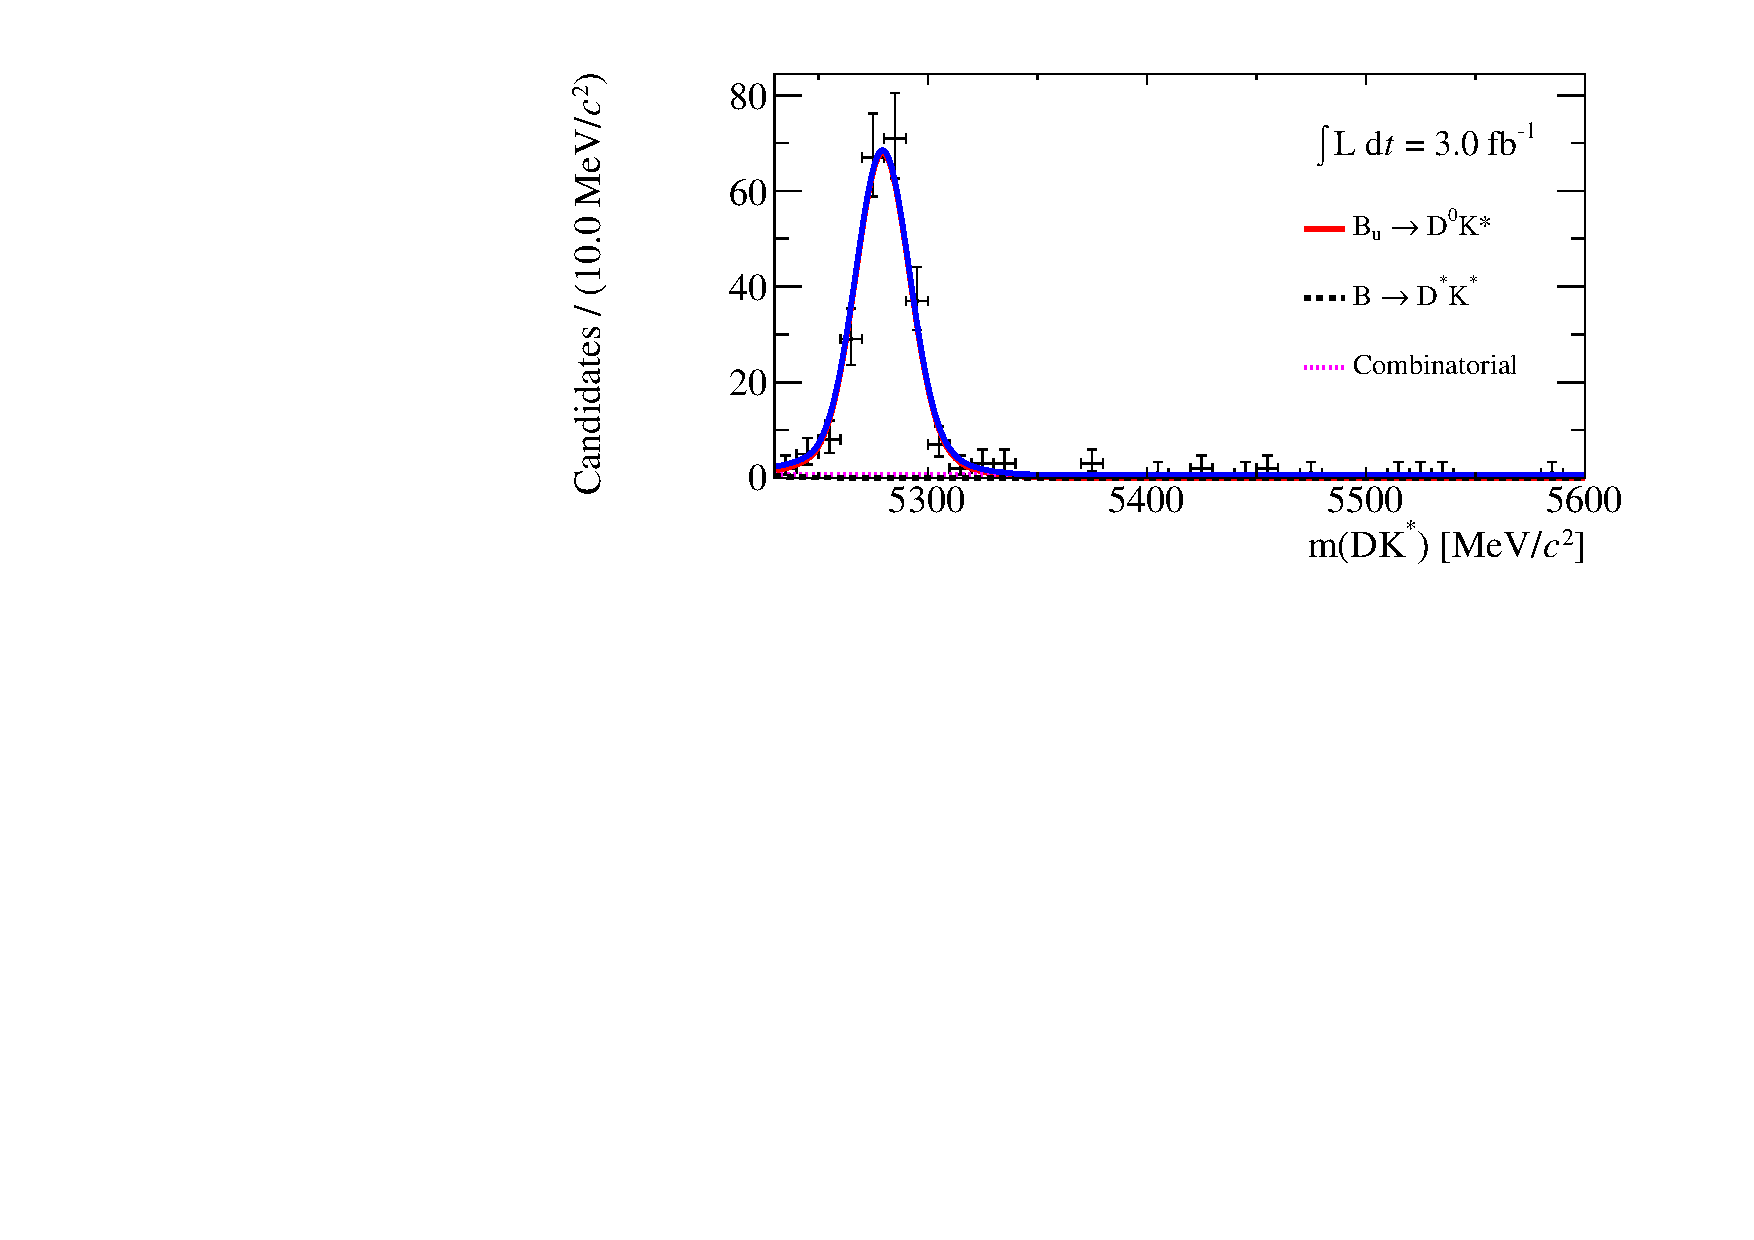
\includegraphics[width=0.25\linewidth]{combinedcanvas_d2kpi_LL_run1.pdf}}
%\hfill
%\subfloat[$KK$, LL]{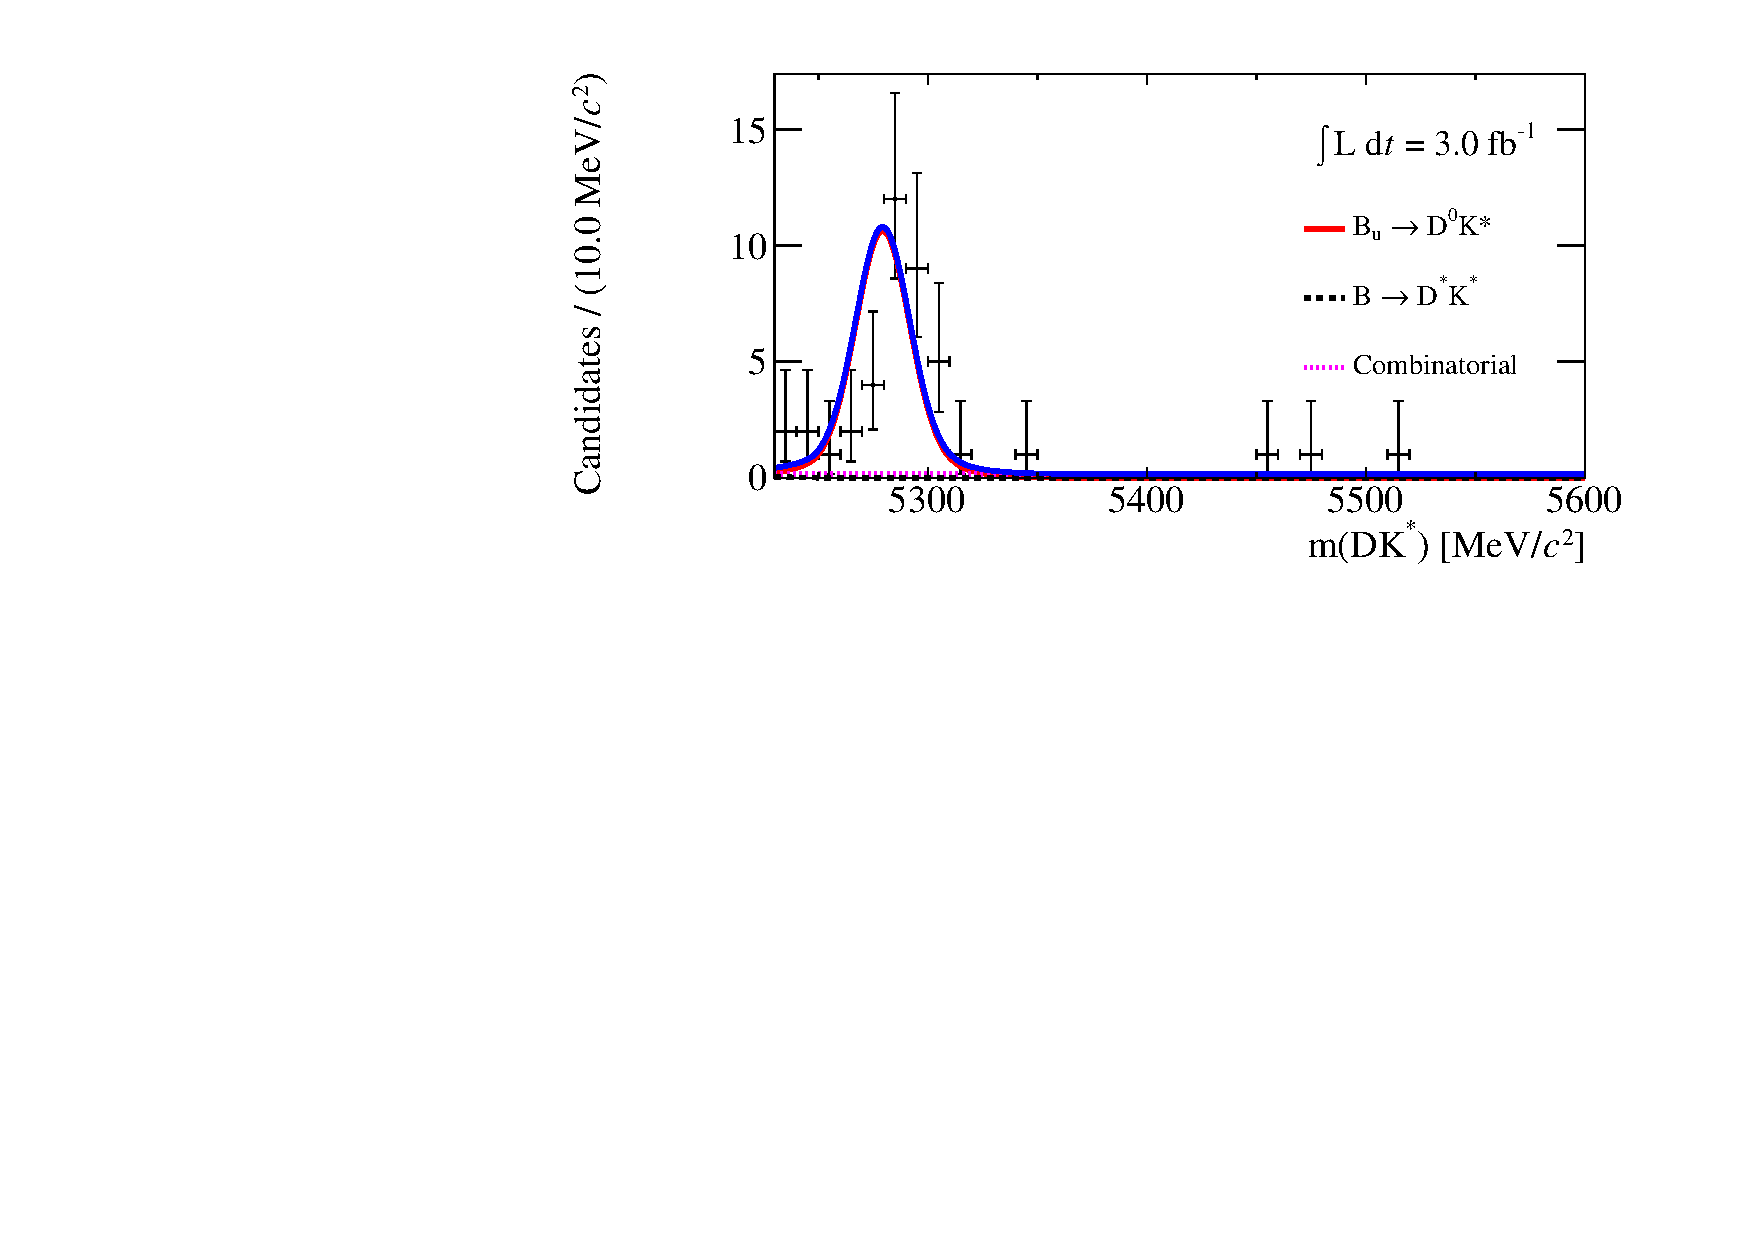
\includegraphics[width=0.25\linewidth]{combinedcanvas_d2kk_LL_run1.pdf}}
%\hfill
%\subfloat[$\pi\pi$, LL]{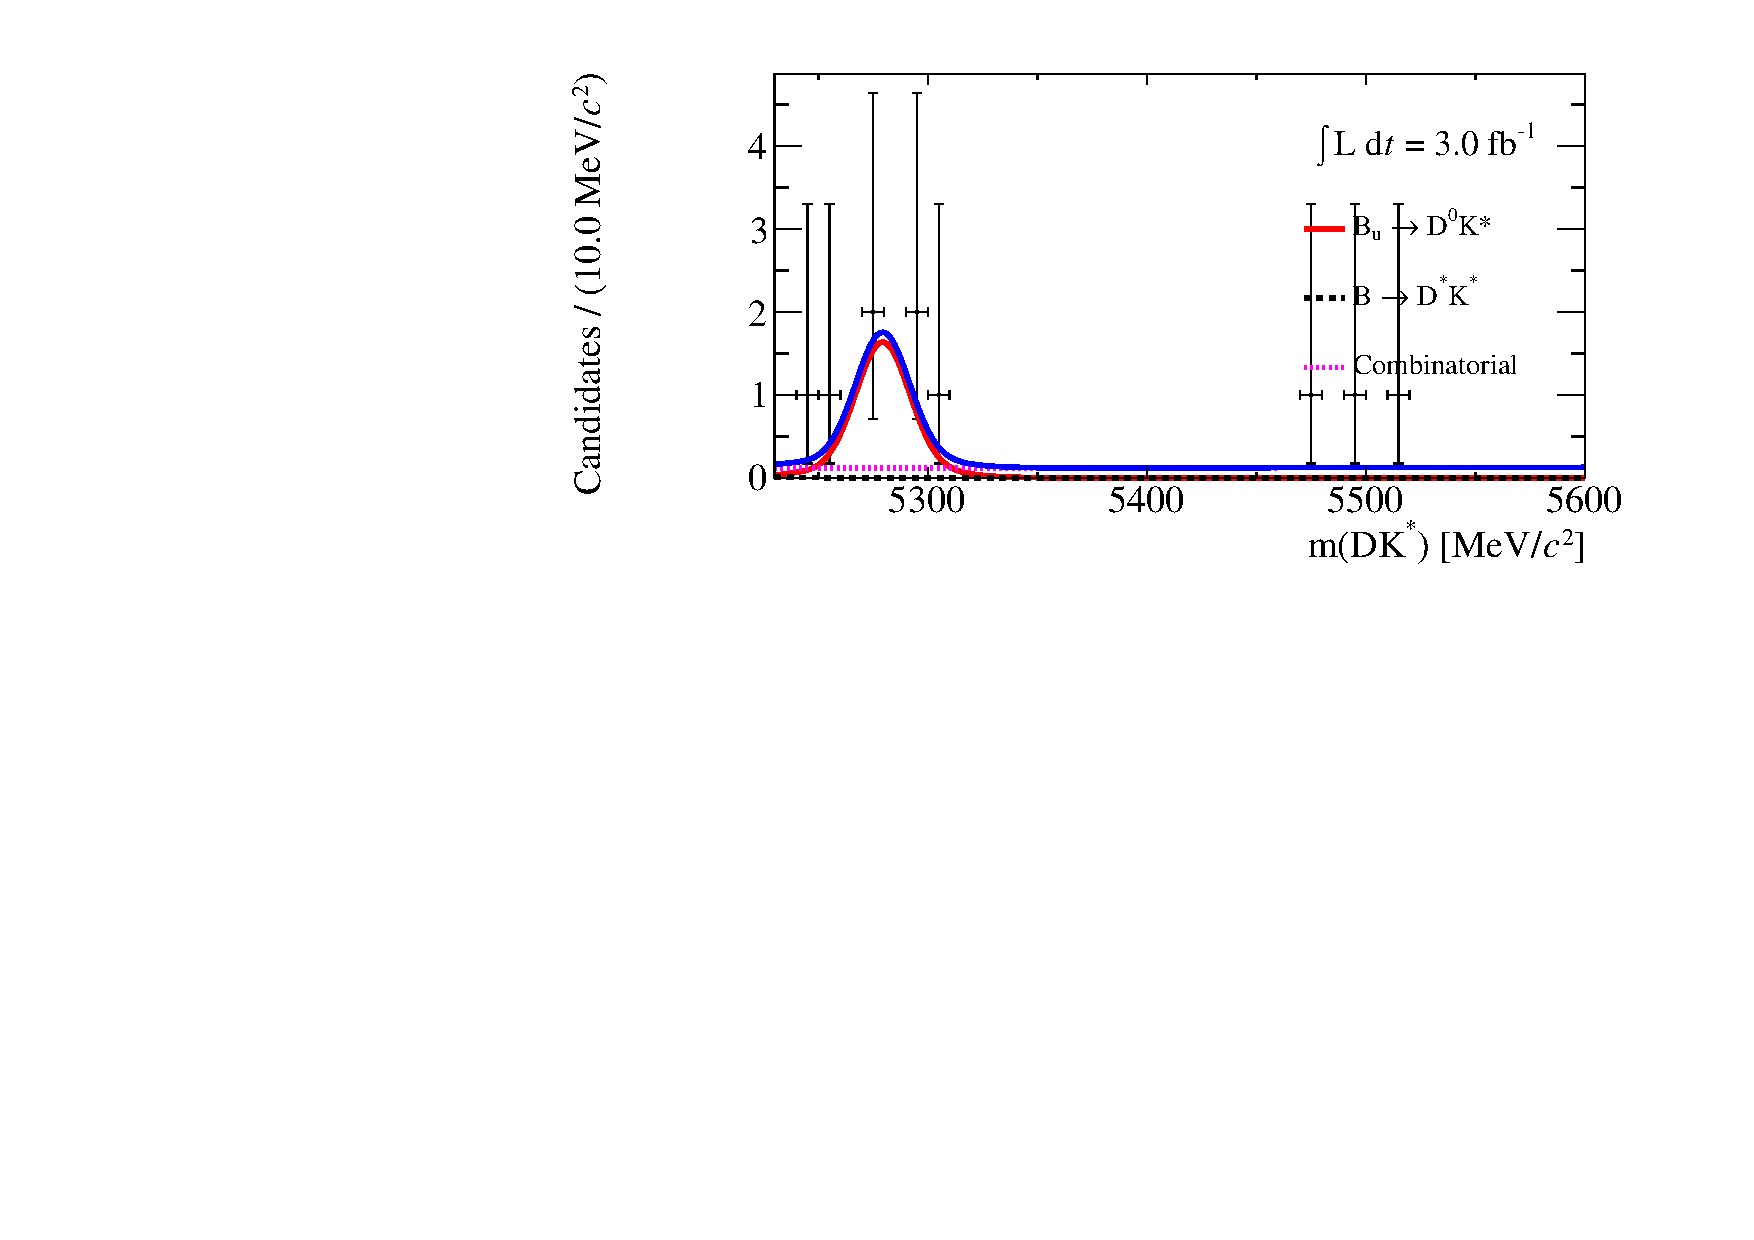
\includegraphics[width=0.25\linewidth]{combinedcanvas_d2pipi_LL_run1.pdf}}
%\hfill
%\subfloat[$\pi K$, LL]{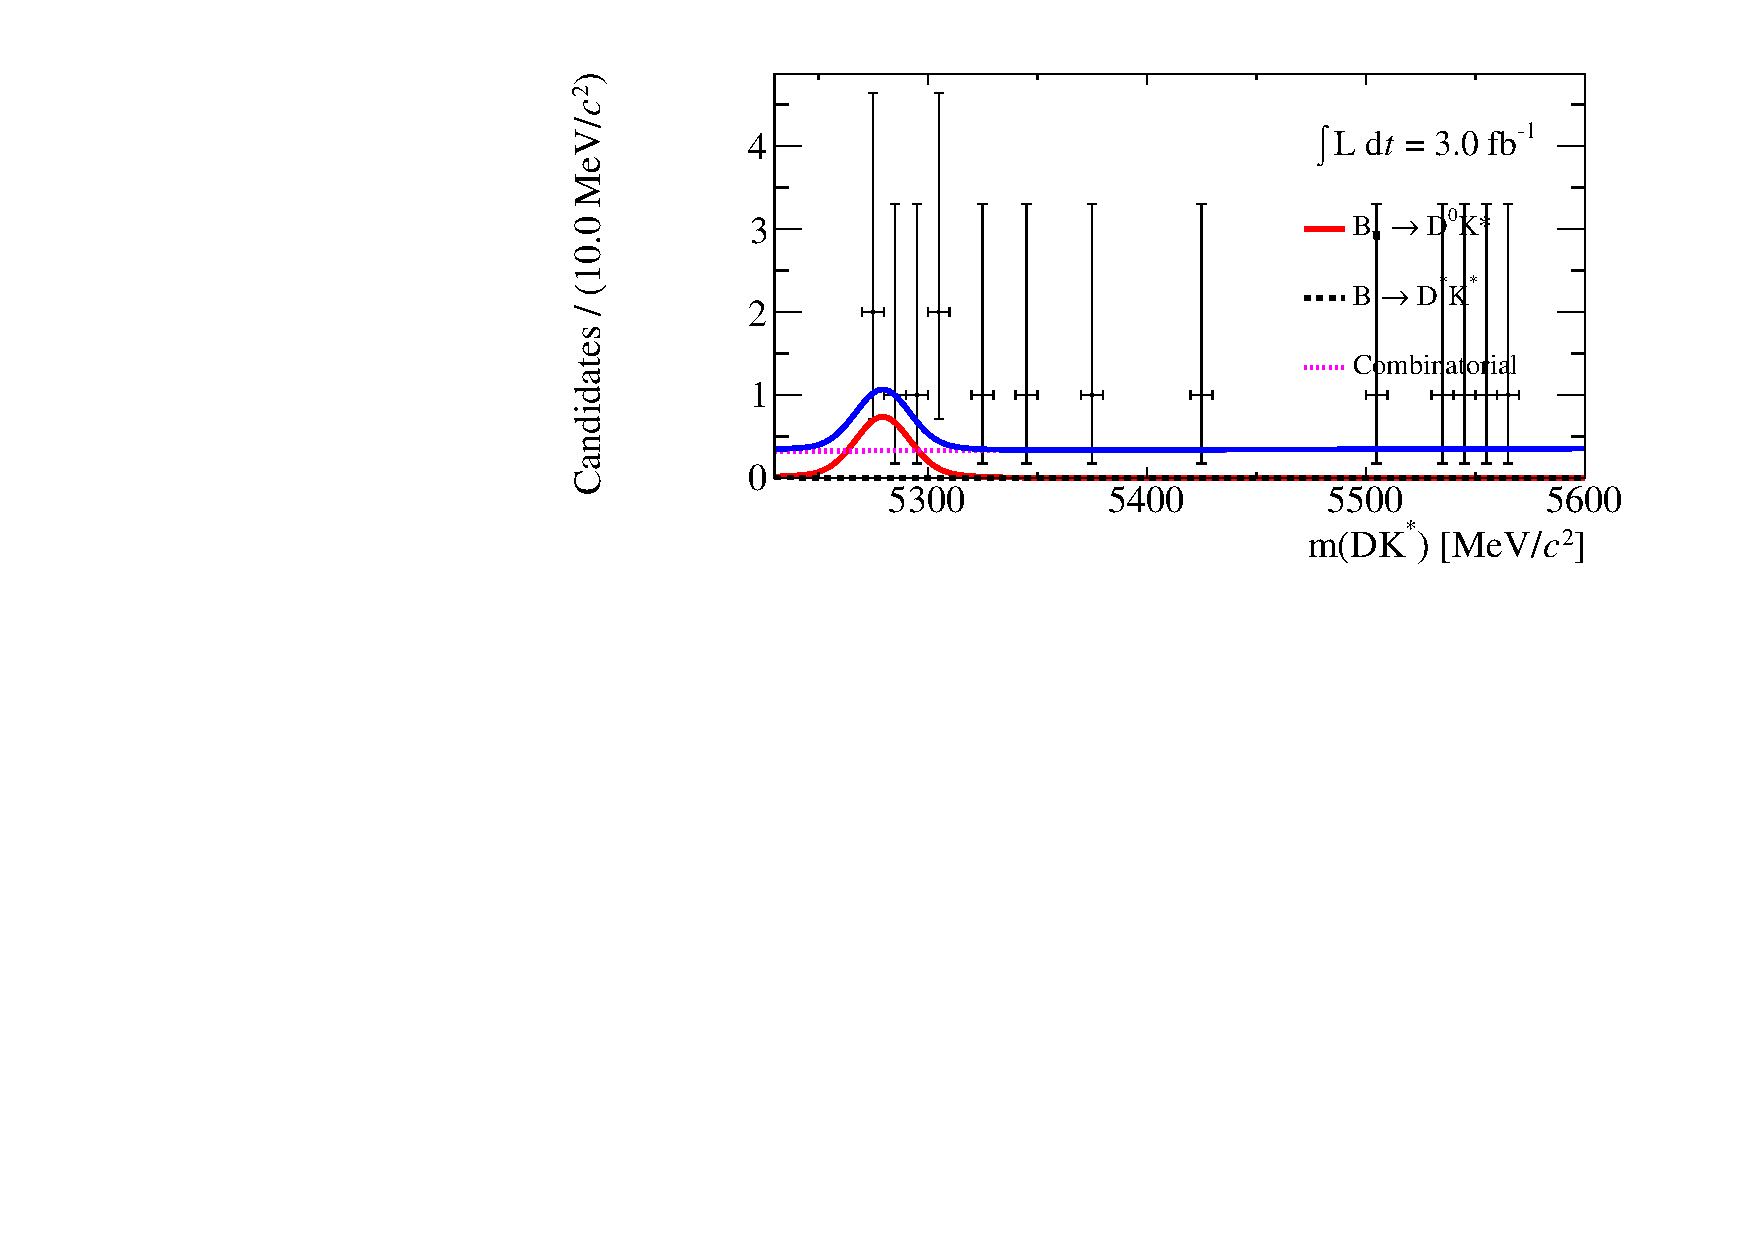
\includegraphics[width=0.25\linewidth]{combinedcanvas_d2pik_LL_run1.pdf}}
%\hfill
%\subfloat[$K\pi$, DD]{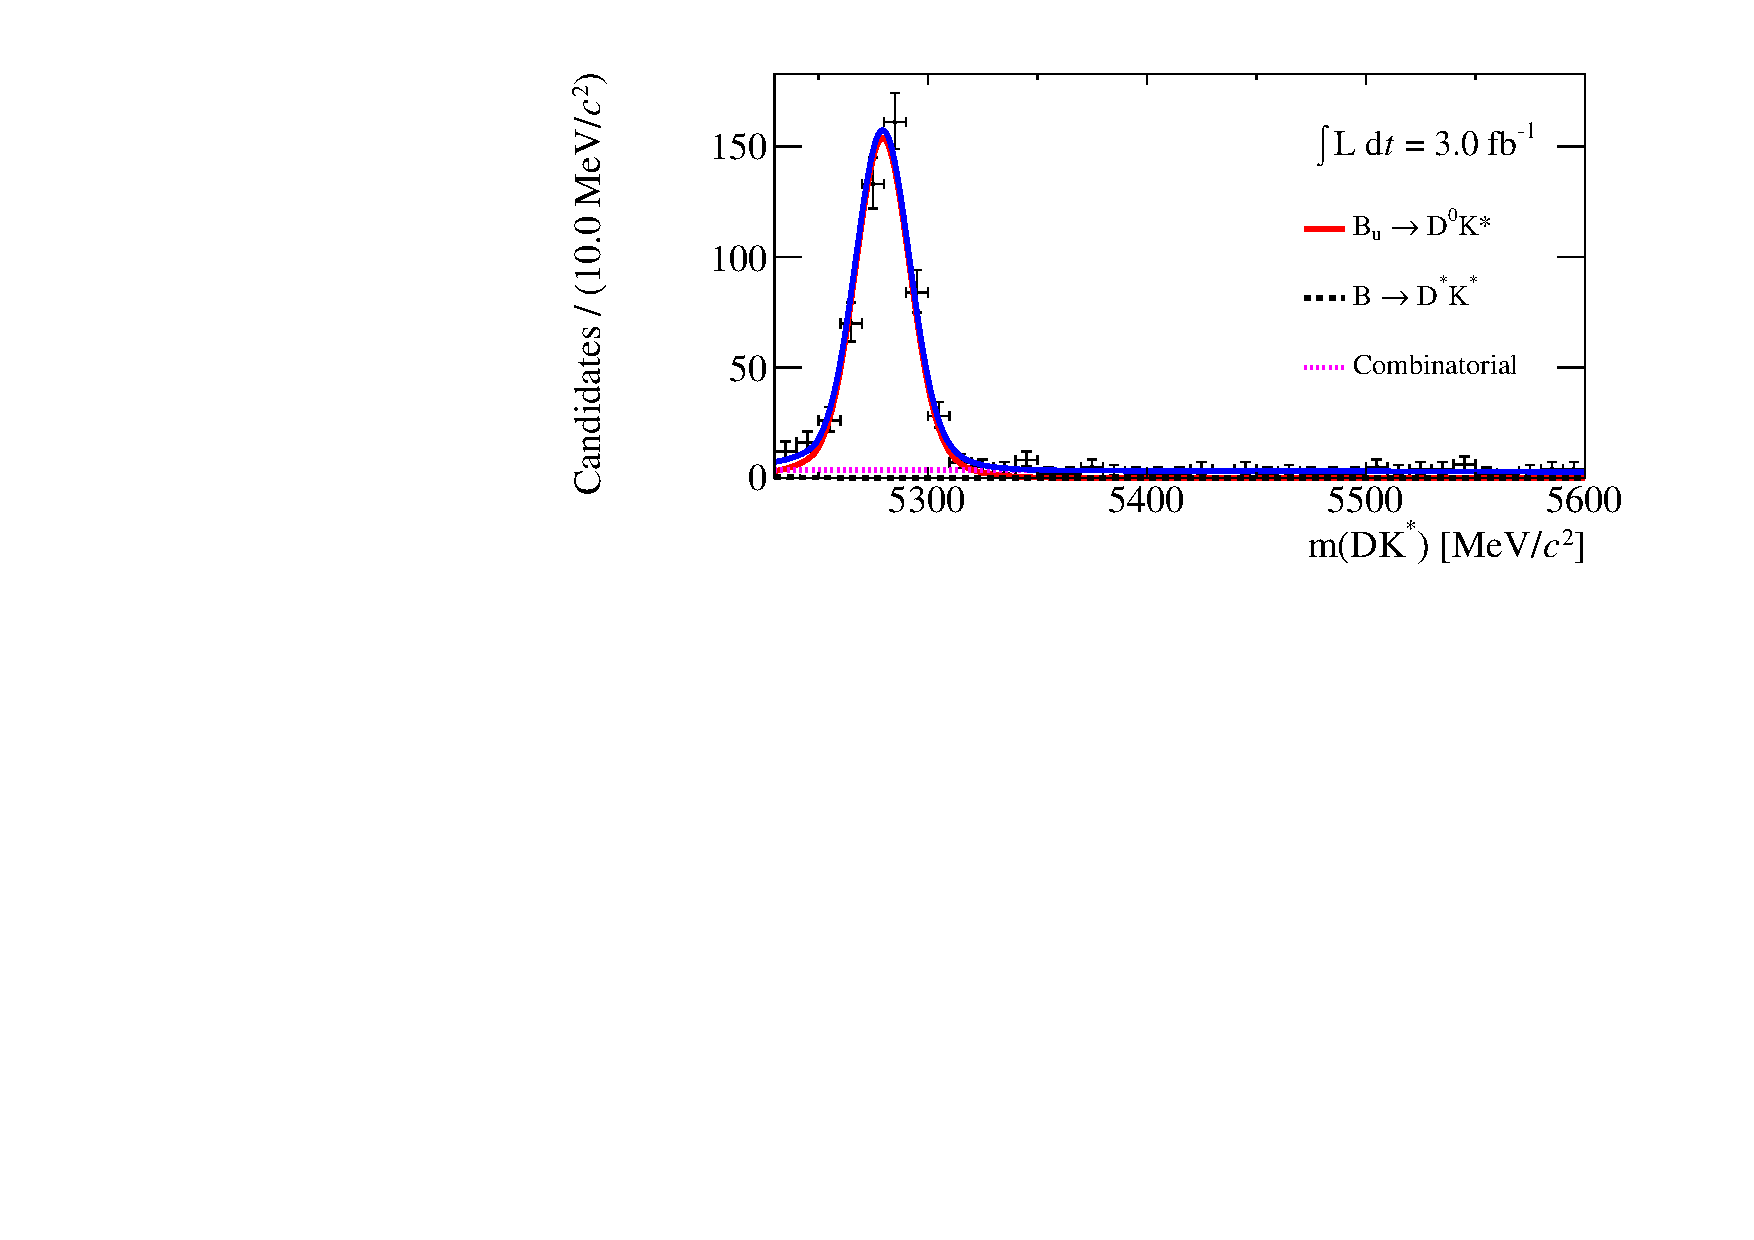
\includegraphics[width=0.25\linewidth]{combinedcanvas_d2kpi_DD_run1.pdf}}
%\hfill
%\subfloat[$KK$, DD]{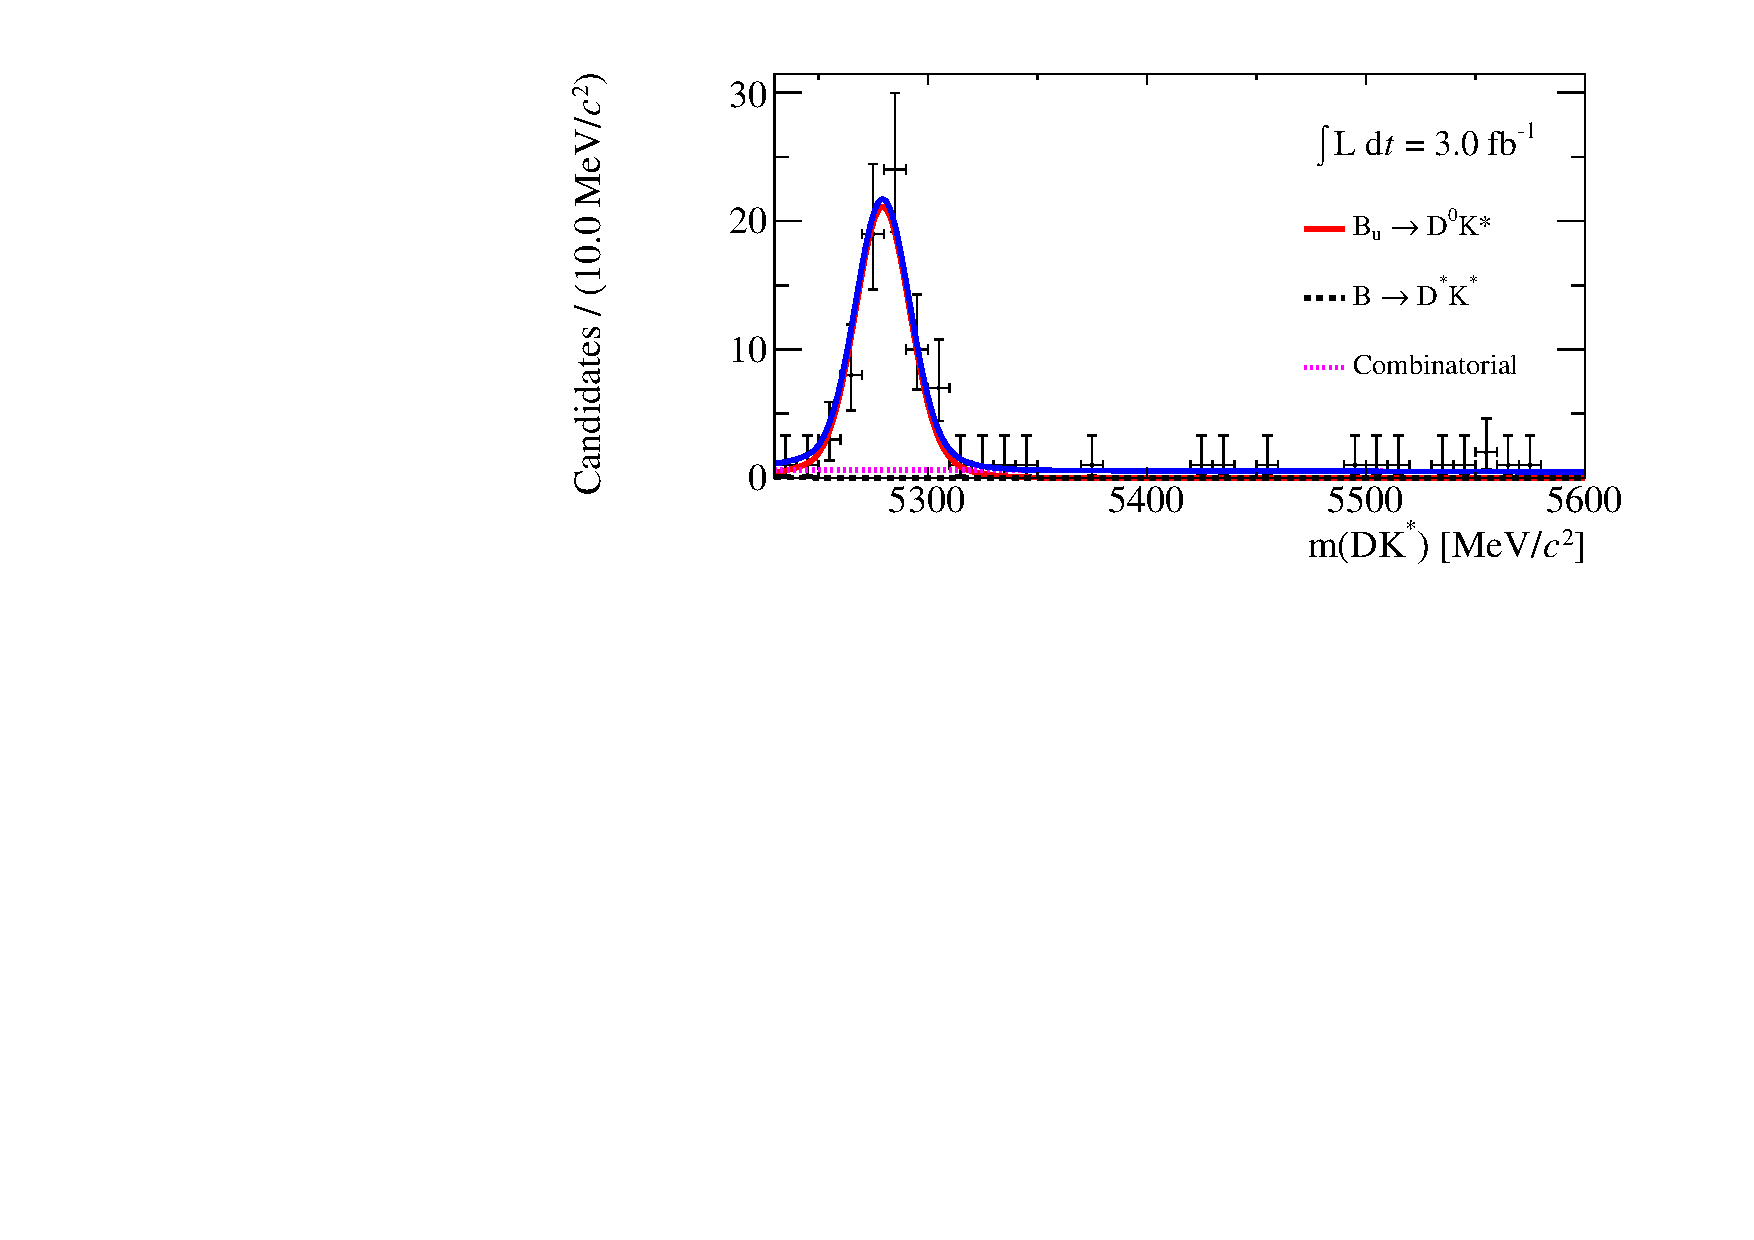
\includegraphics[width=0.25\linewidth]{combinedcanvas_d2kk_DD_run1.pdf}}
%\hfill
%\subfloat[$\pi\pi$, DD]{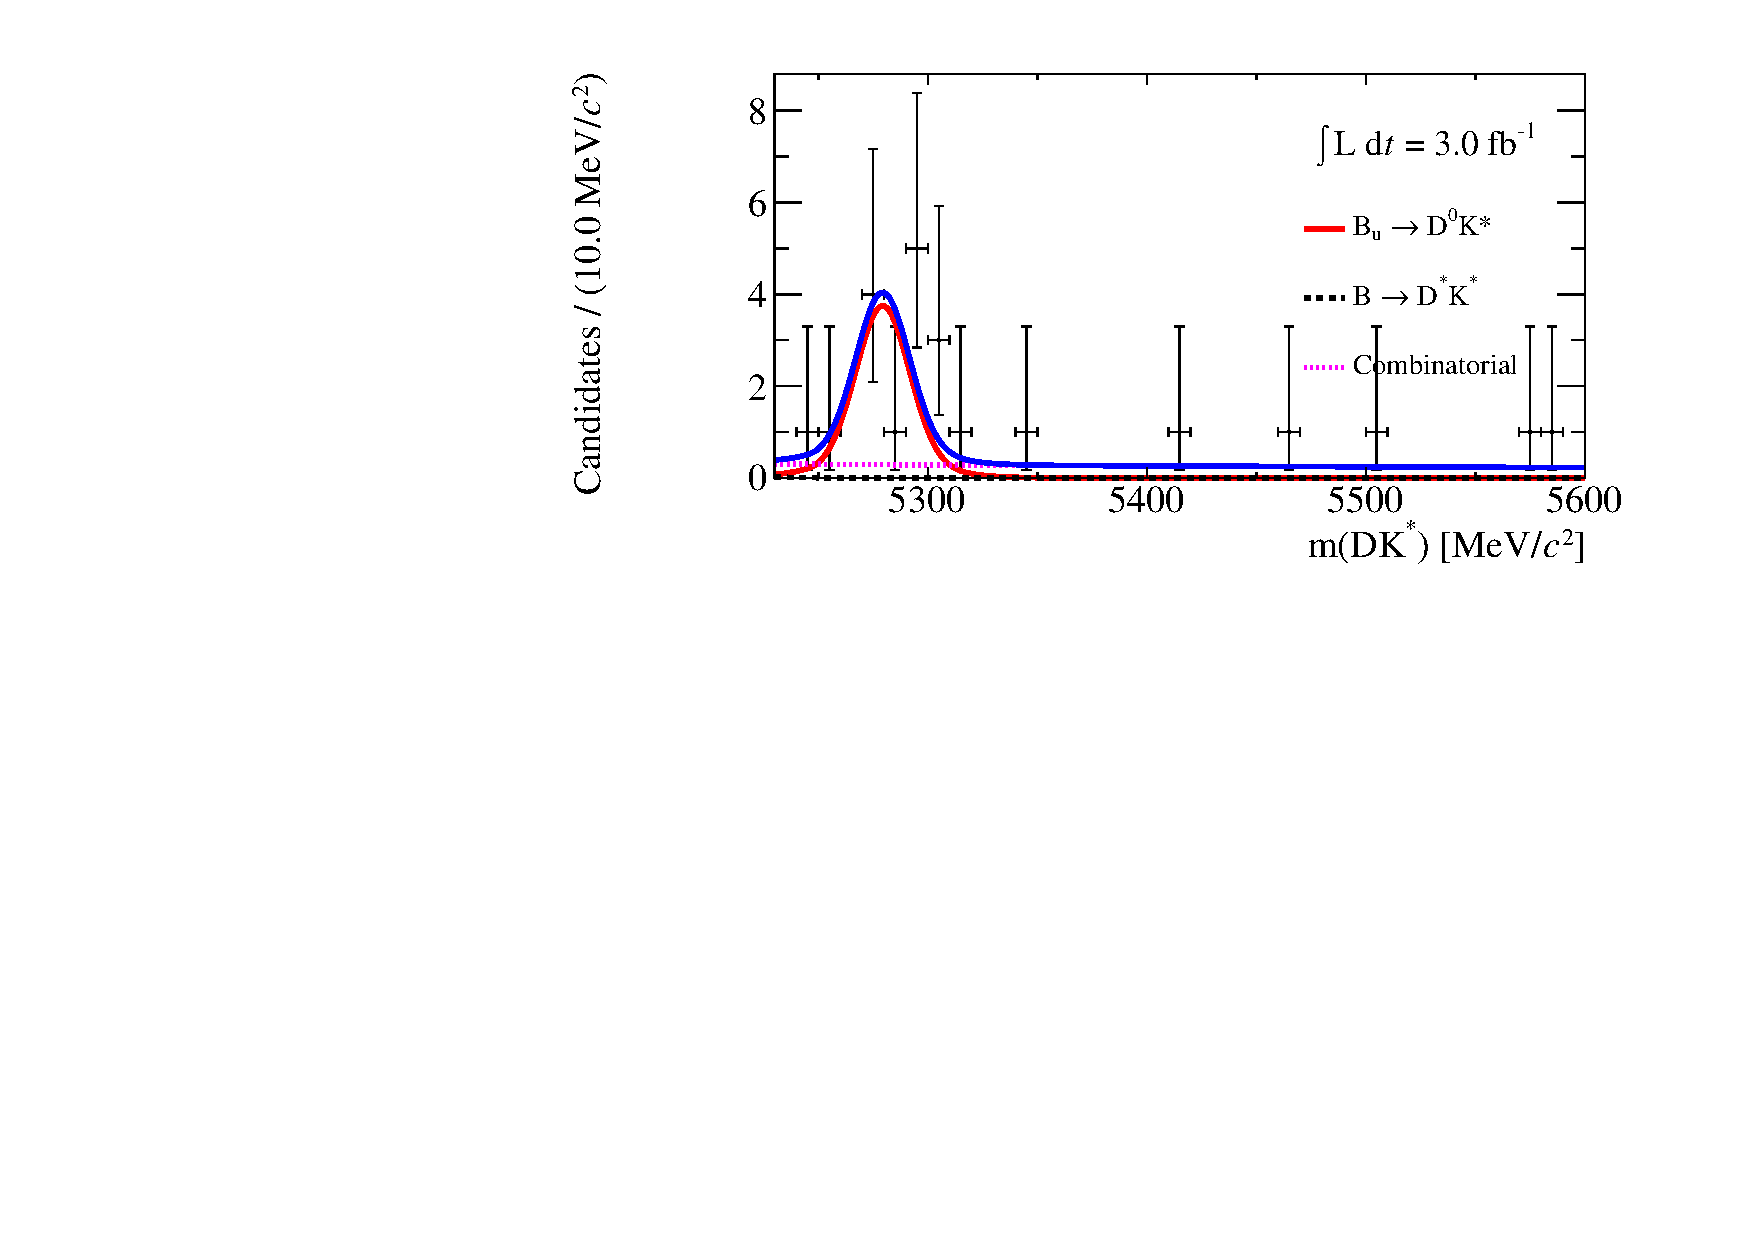
\includegraphics[width=0.25\linewidth]{combinedcanvas_d2pipi_DD_run1.pdf}}
%\hfill
%\subfloat[$\pi K$, DD]{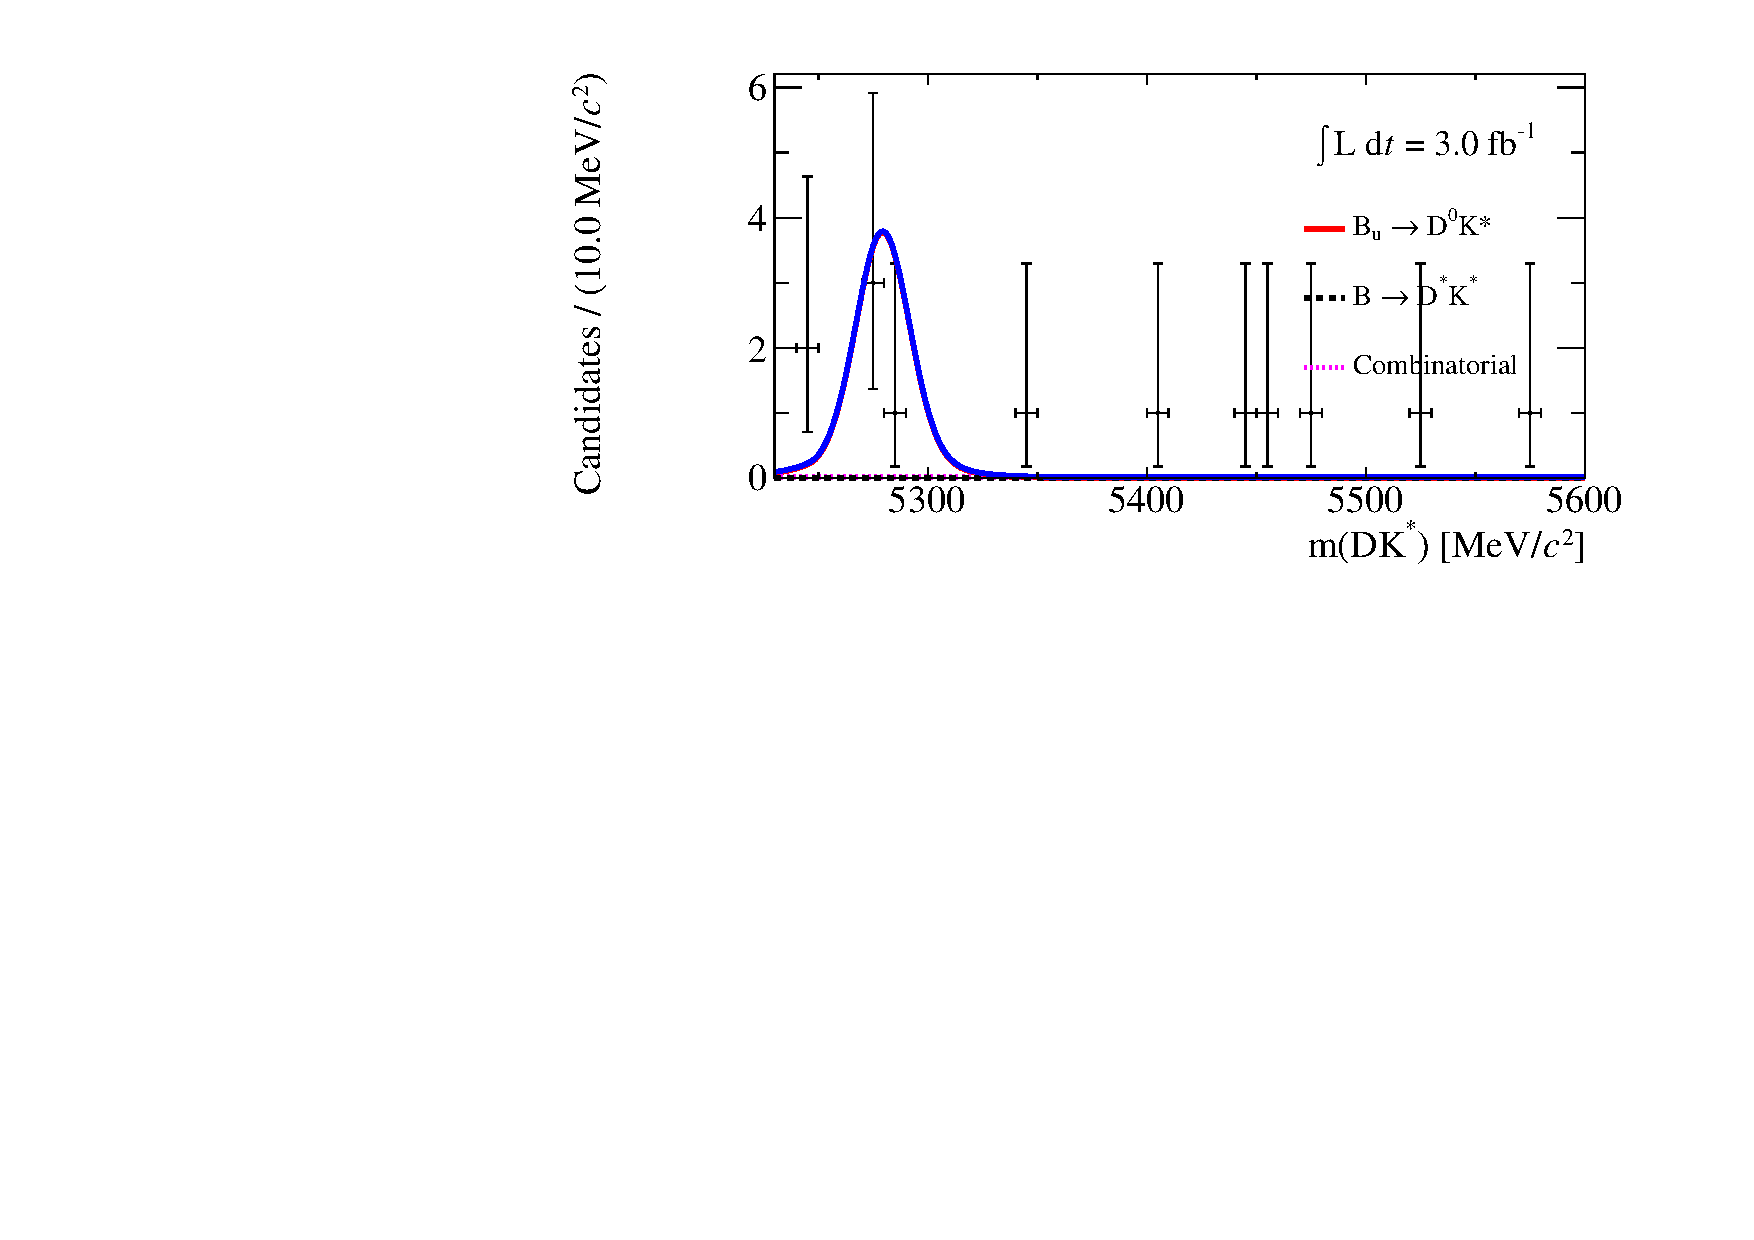
\includegraphics[width=0.25\linewidth]{combinedcanvas_d2pik_DD_run1.pdf}}
%\hfill
%\subfloat[$K\pi\pi\pi$, LL]{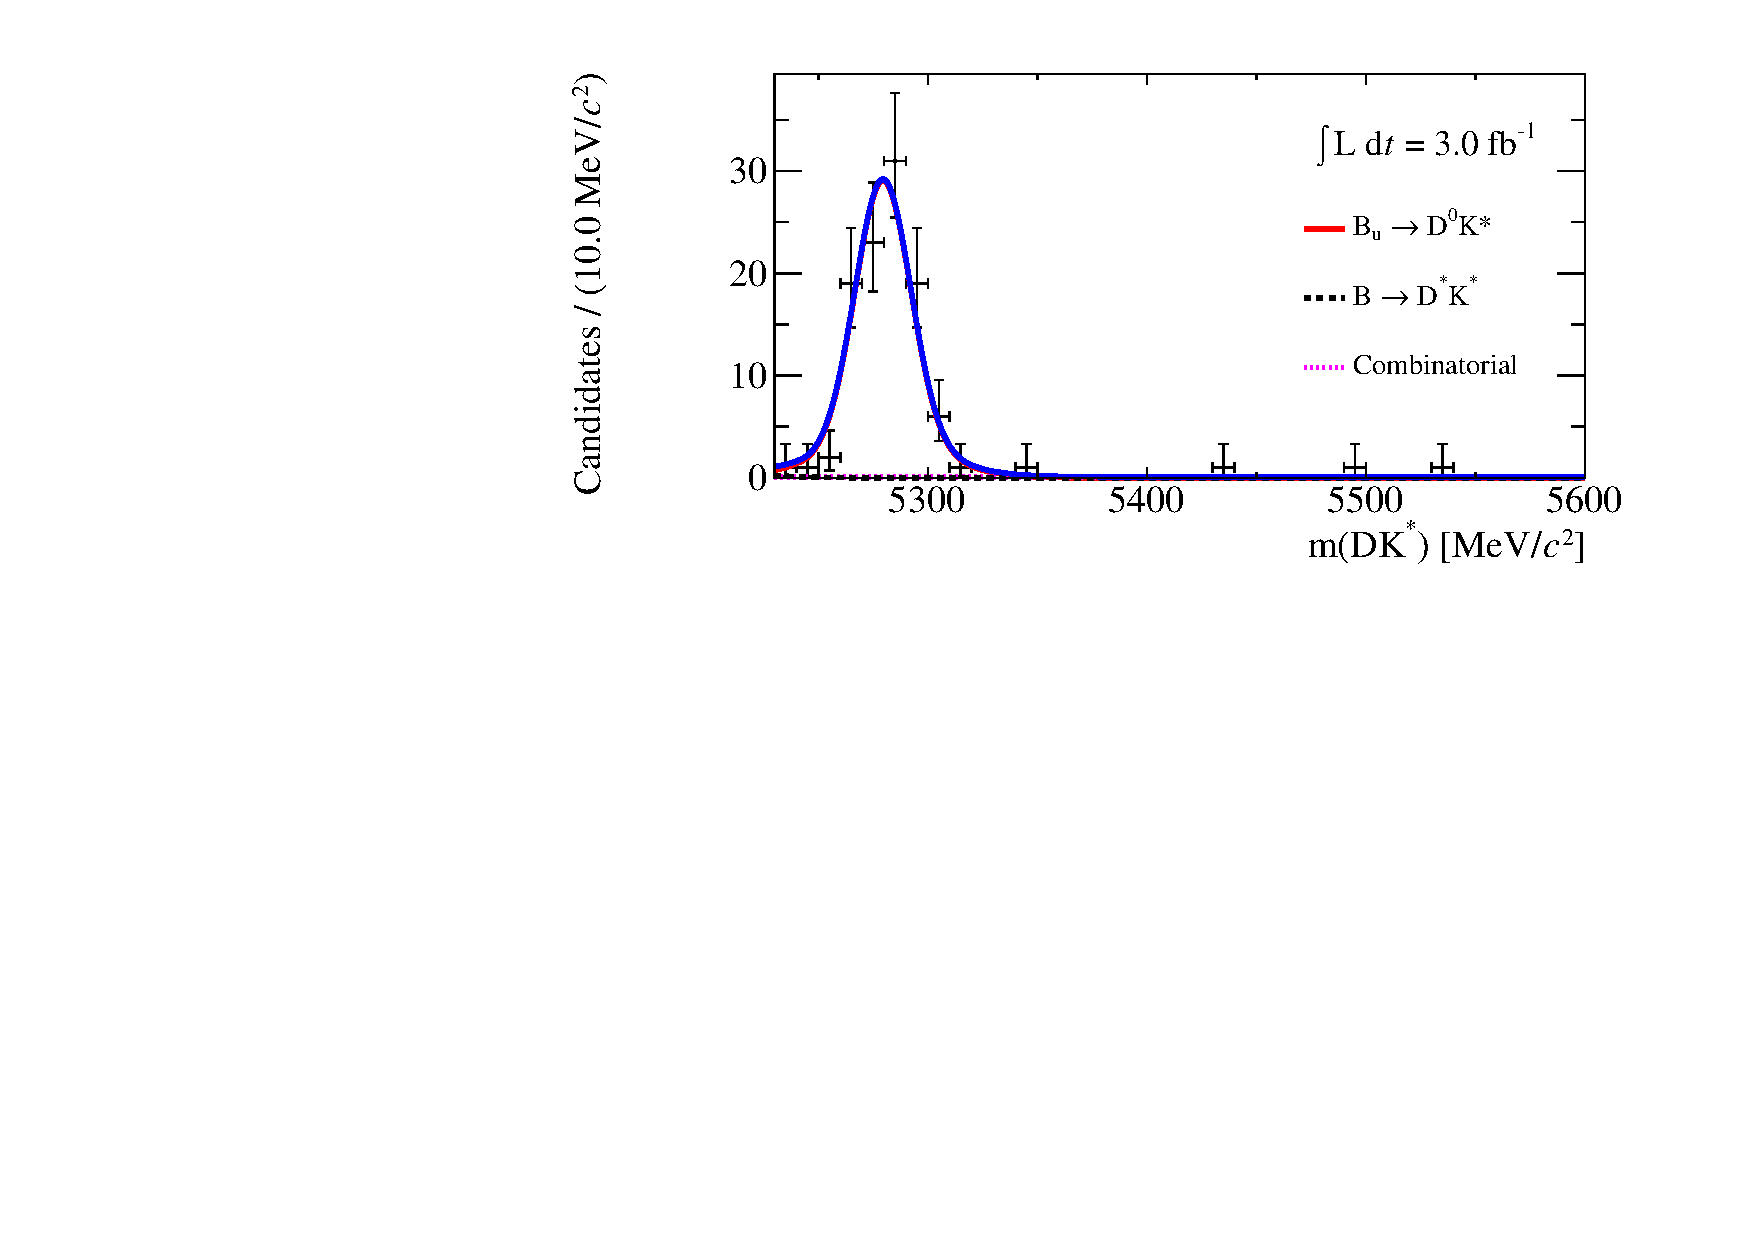
\includegraphics[width=0.26\linewidth]{combinedcanvas_d2kpipipi_LL_run1.pdf}}
%\subfloat[$\pi\pi\pi\pi$, LL]{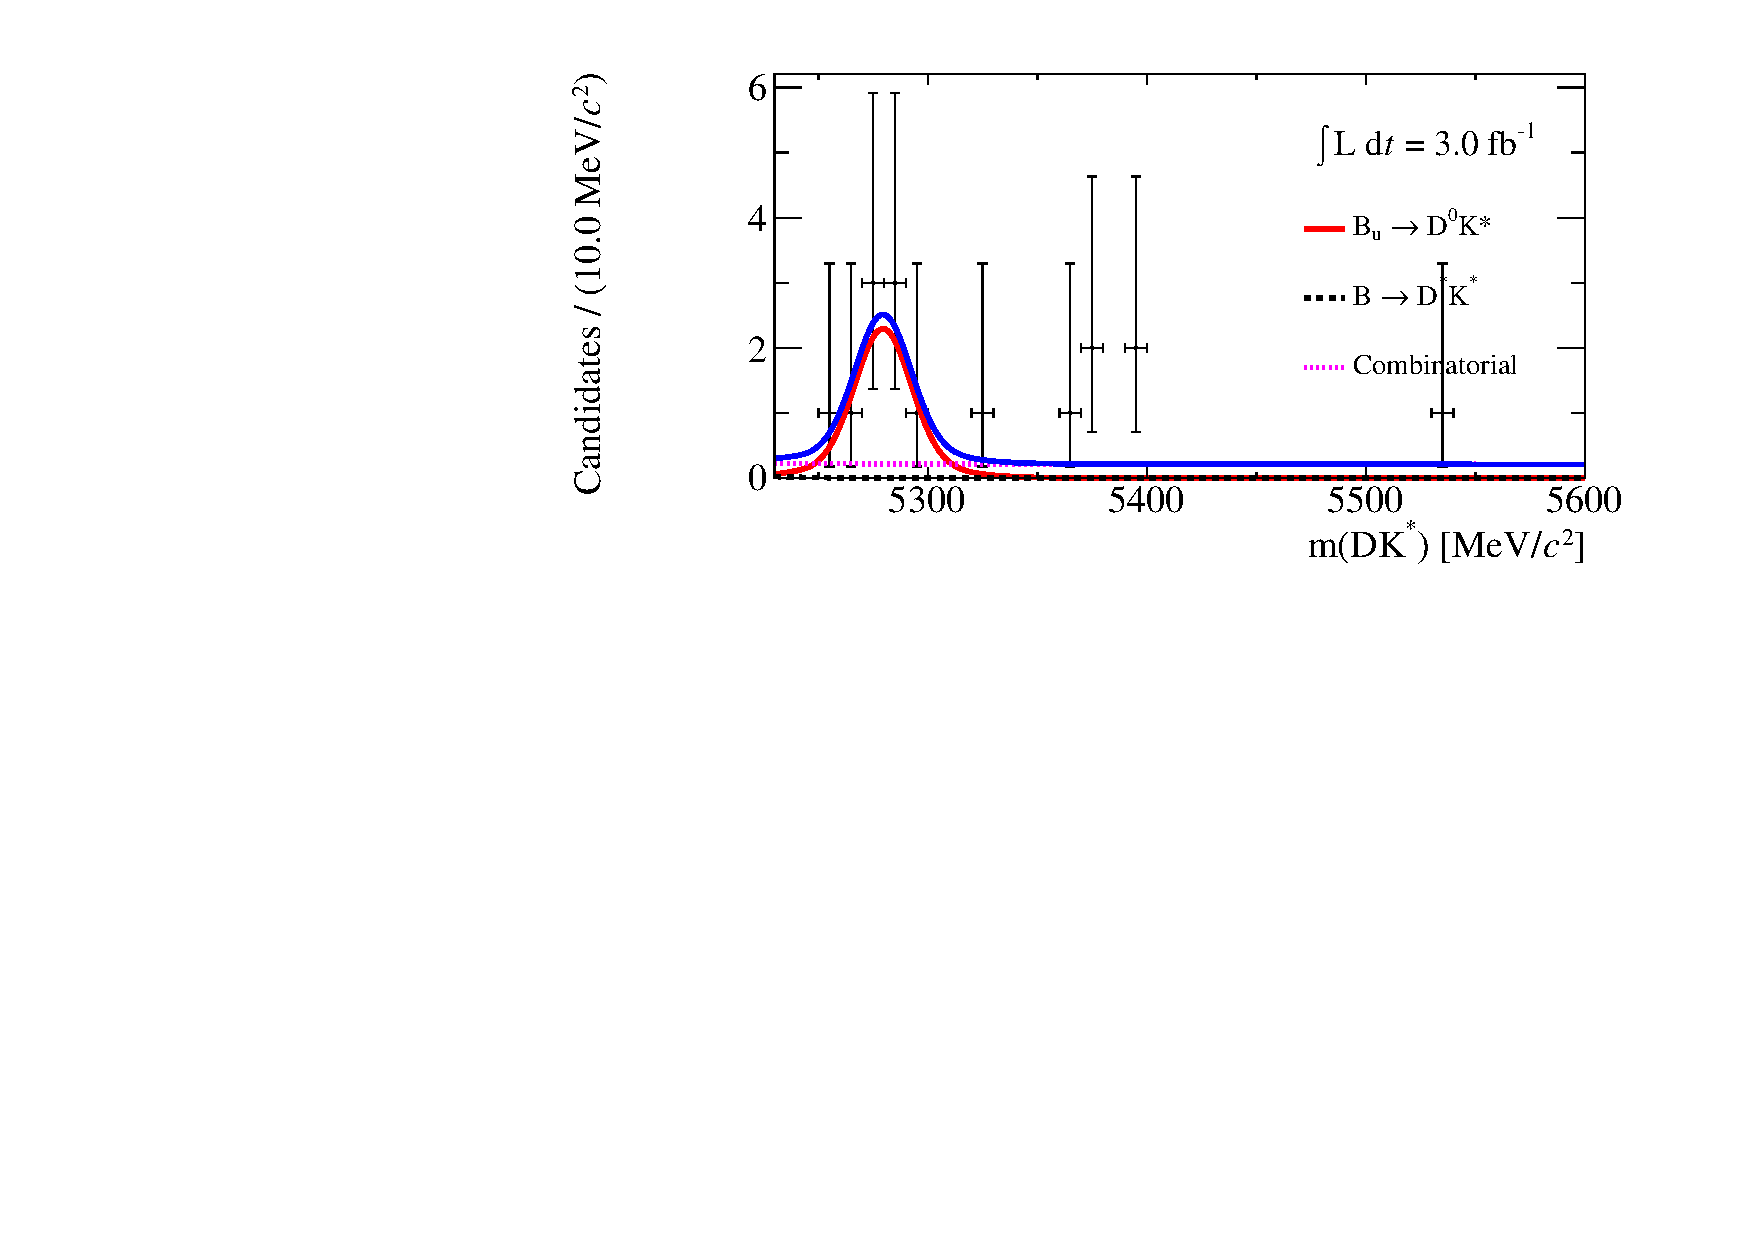
\includegraphics[width=0.26\linewidth]{combinedcanvas_d2pipipipi_LL_run1.pdf}}
%\subfloat[$\pi K\pi\pi$, LL]{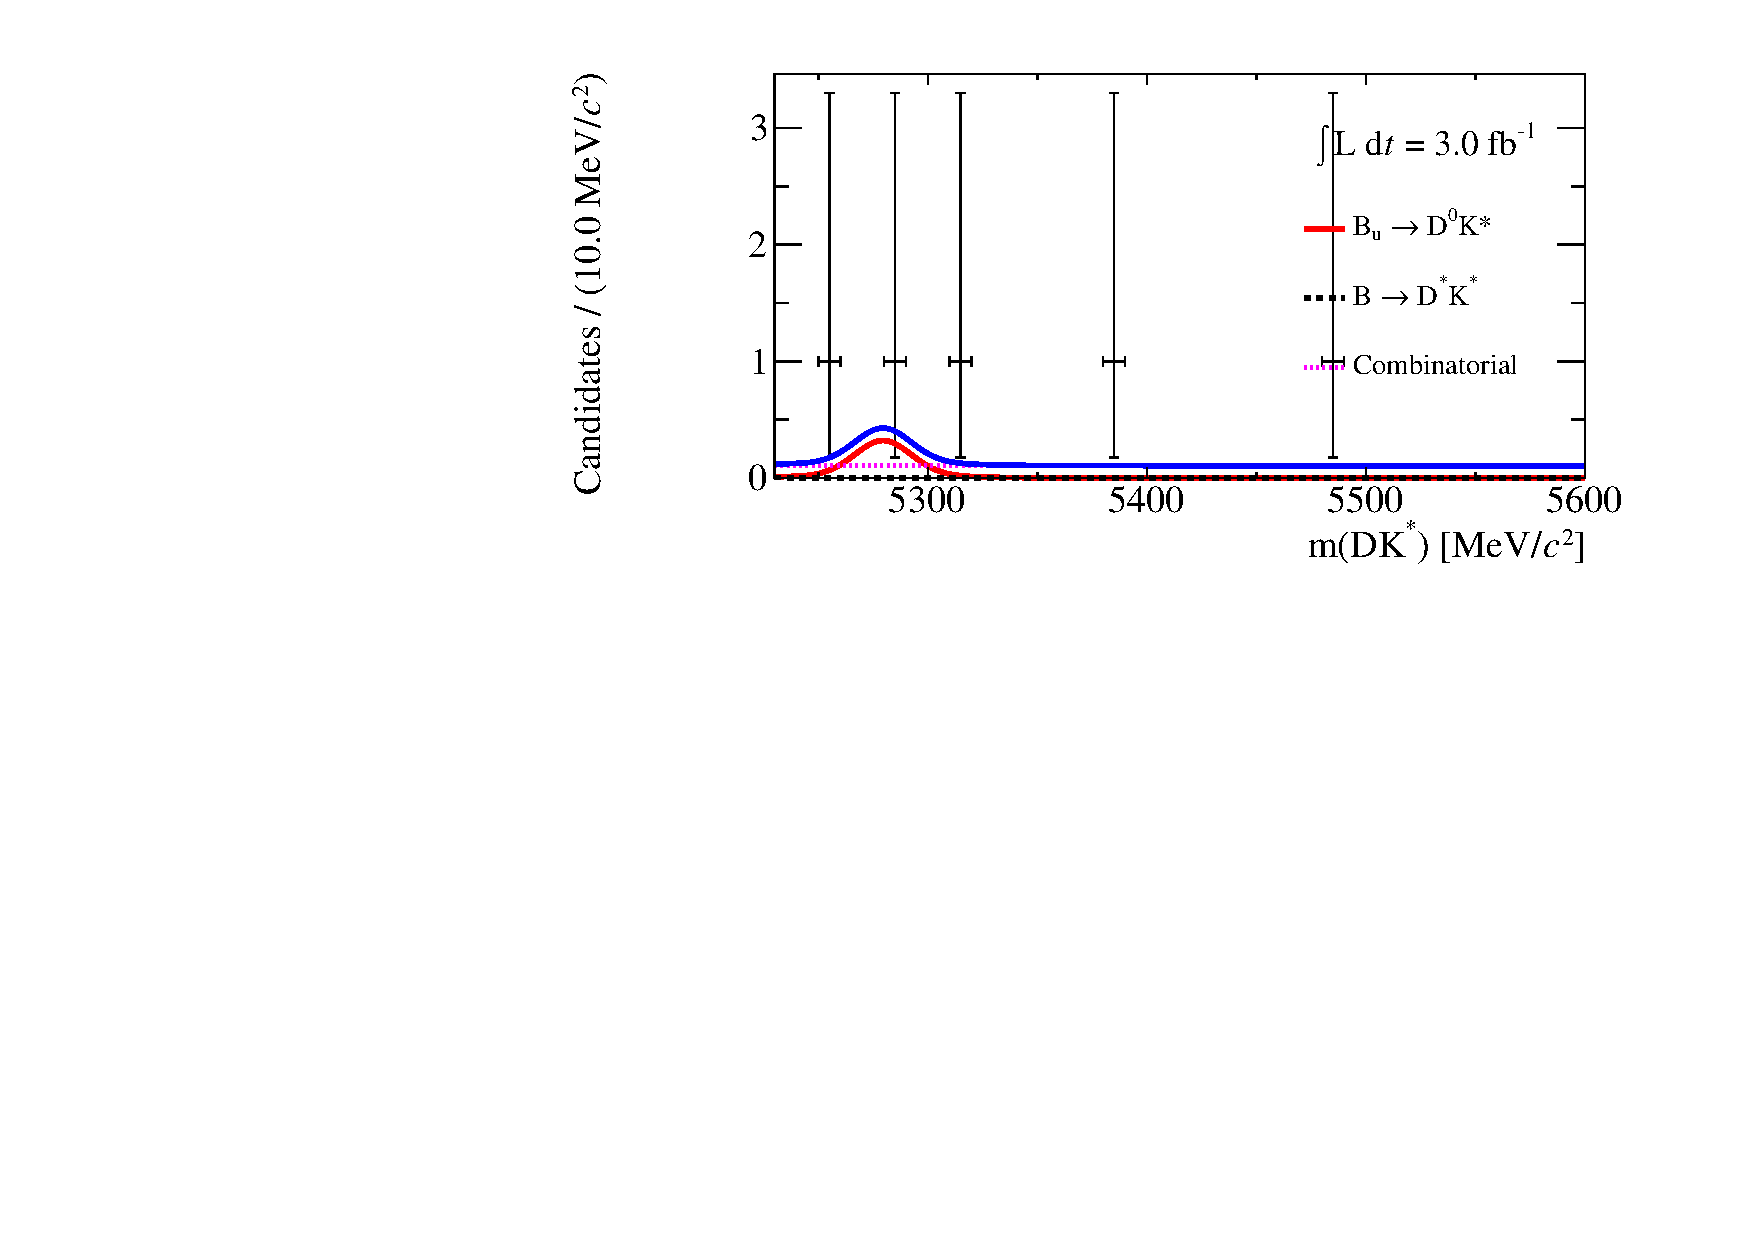
\includegraphics[width=0.26\linewidth]{combinedcanvas_d2pikpipi_LL_run1.pdf}}
%\hfill
%\subfloat[$K\pi\pi\pi$, DD]{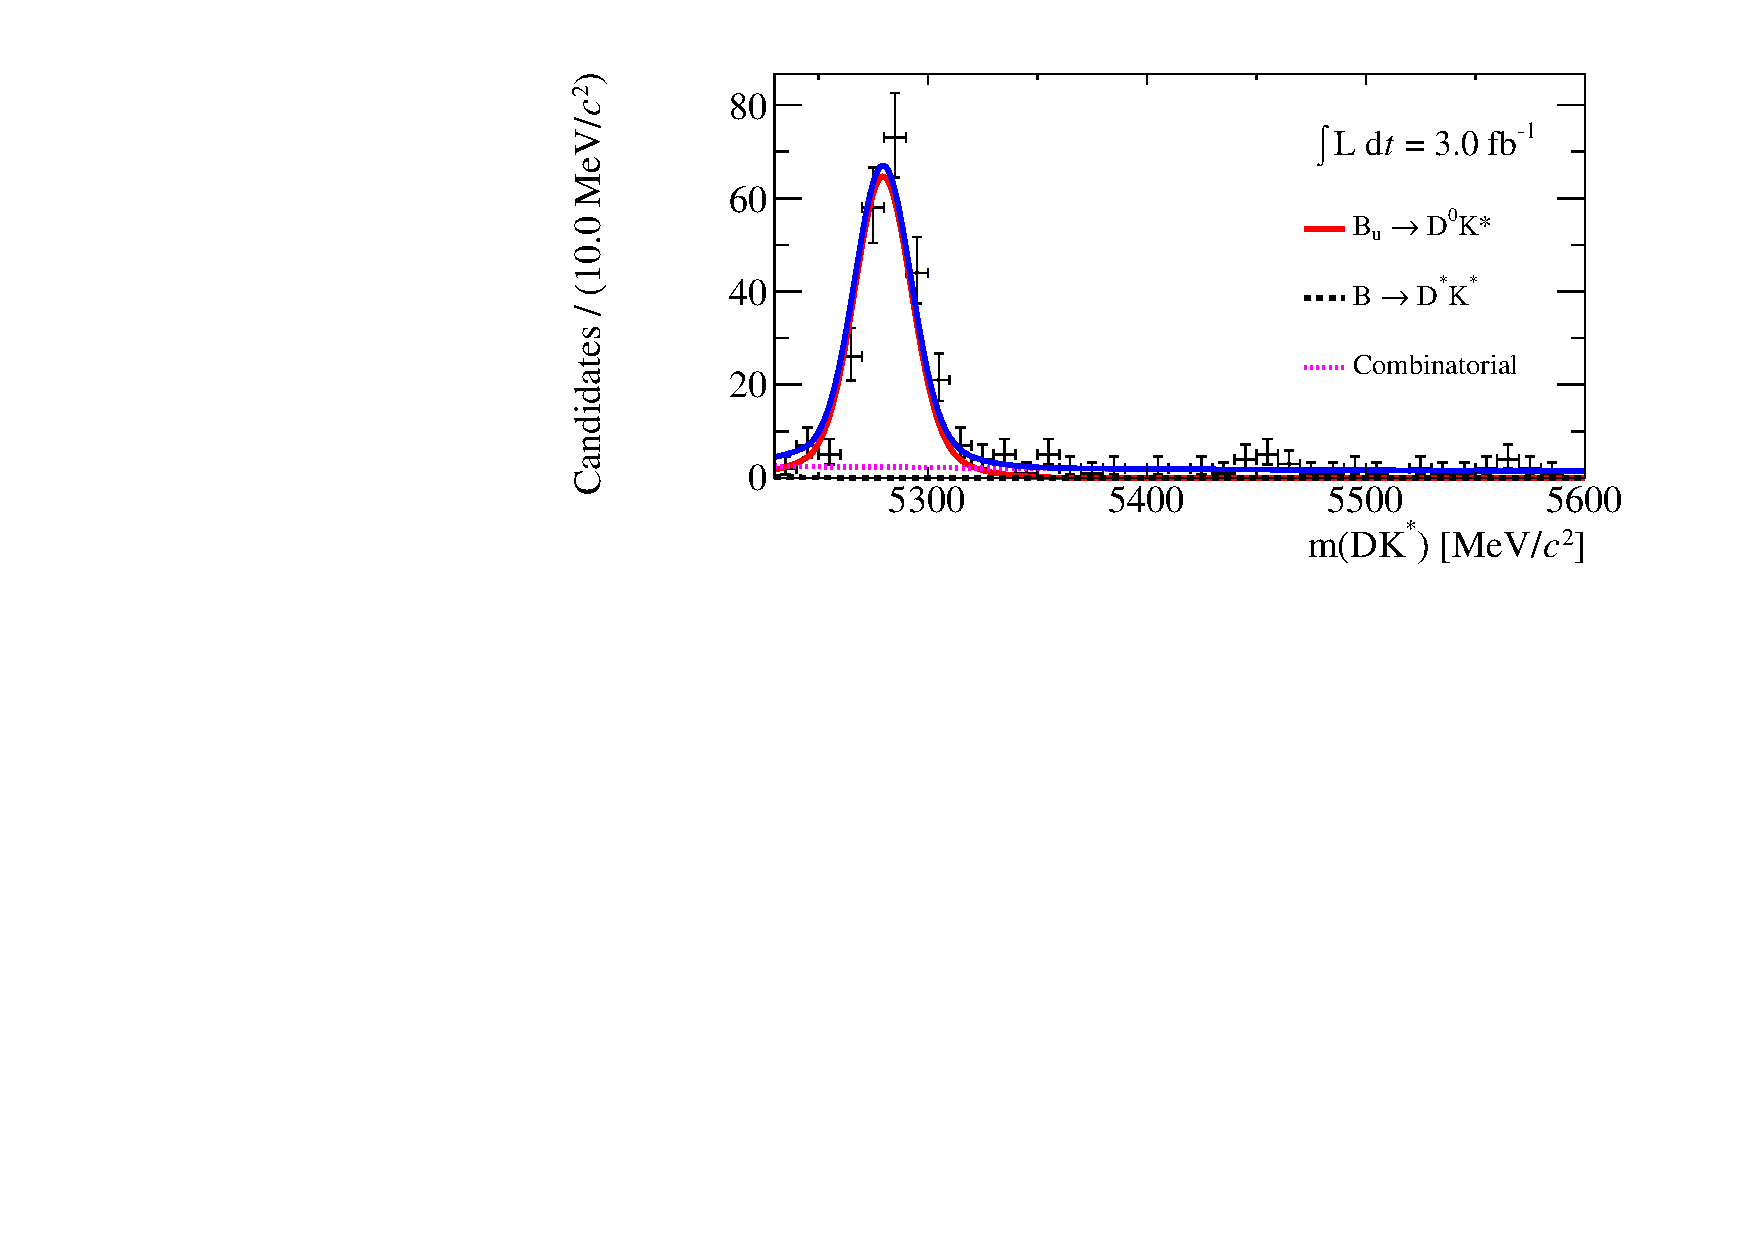
\includegraphics[width=0.26\linewidth]{combinedcanvas_d2kpipipi_DD_run1.pdf}}
%\subfloat[$\pi\pi\pi\pi$, DD]{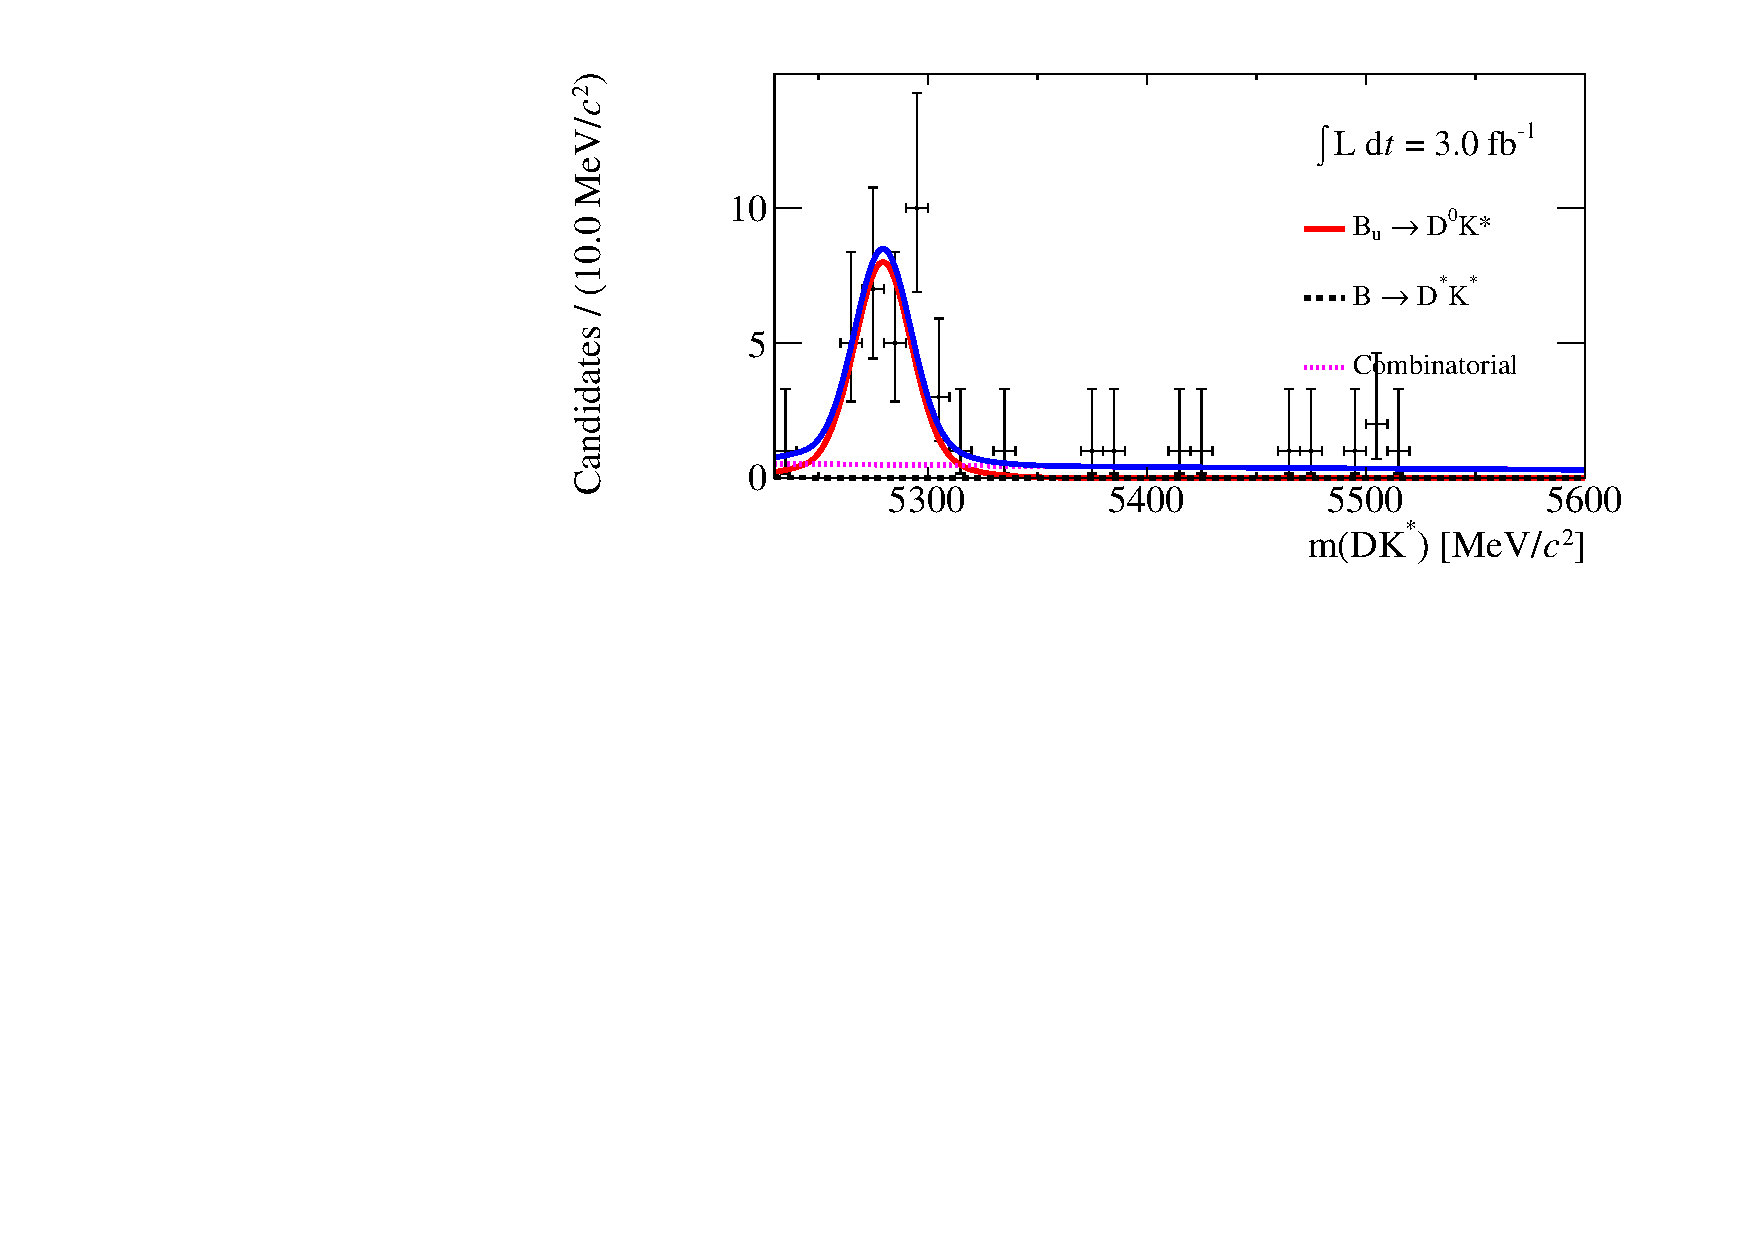
\includegraphics[width=0.26\linewidth]{combinedcanvas_d2pipipipi_DD_run1.pdf}}
%\subfloat[$\pi K\pi\pi$, DD]{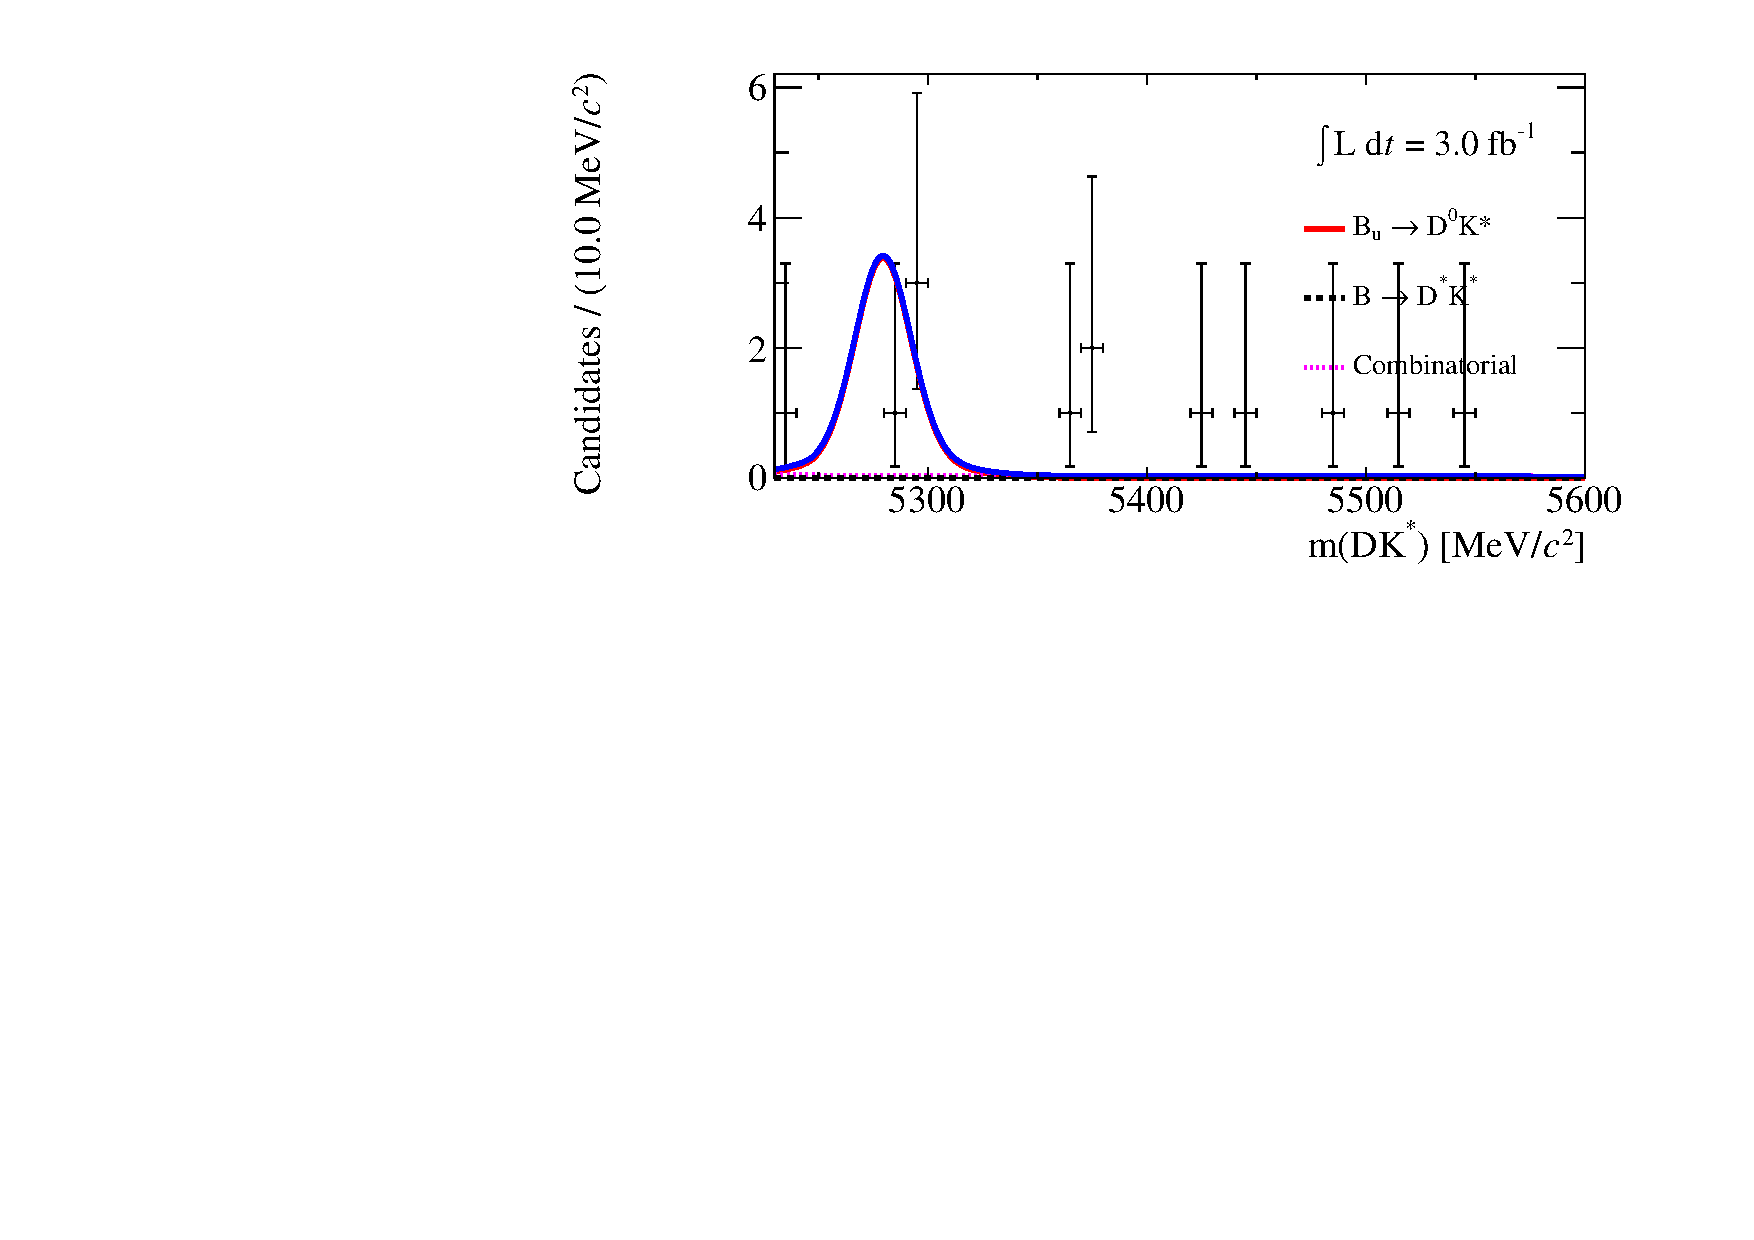
\includegraphics[width=0.26\linewidth]{combinedcanvas_d2pikpipi_DD_run1.pdf}}
%\caption{Results of the simultaneous fit for charged combined Run 1 data}
%\label{datafitcombinedRun1}
%\end{figure}
%
%\begin{figure}
%\centering
%\subfloat[$K\pi$, LL]{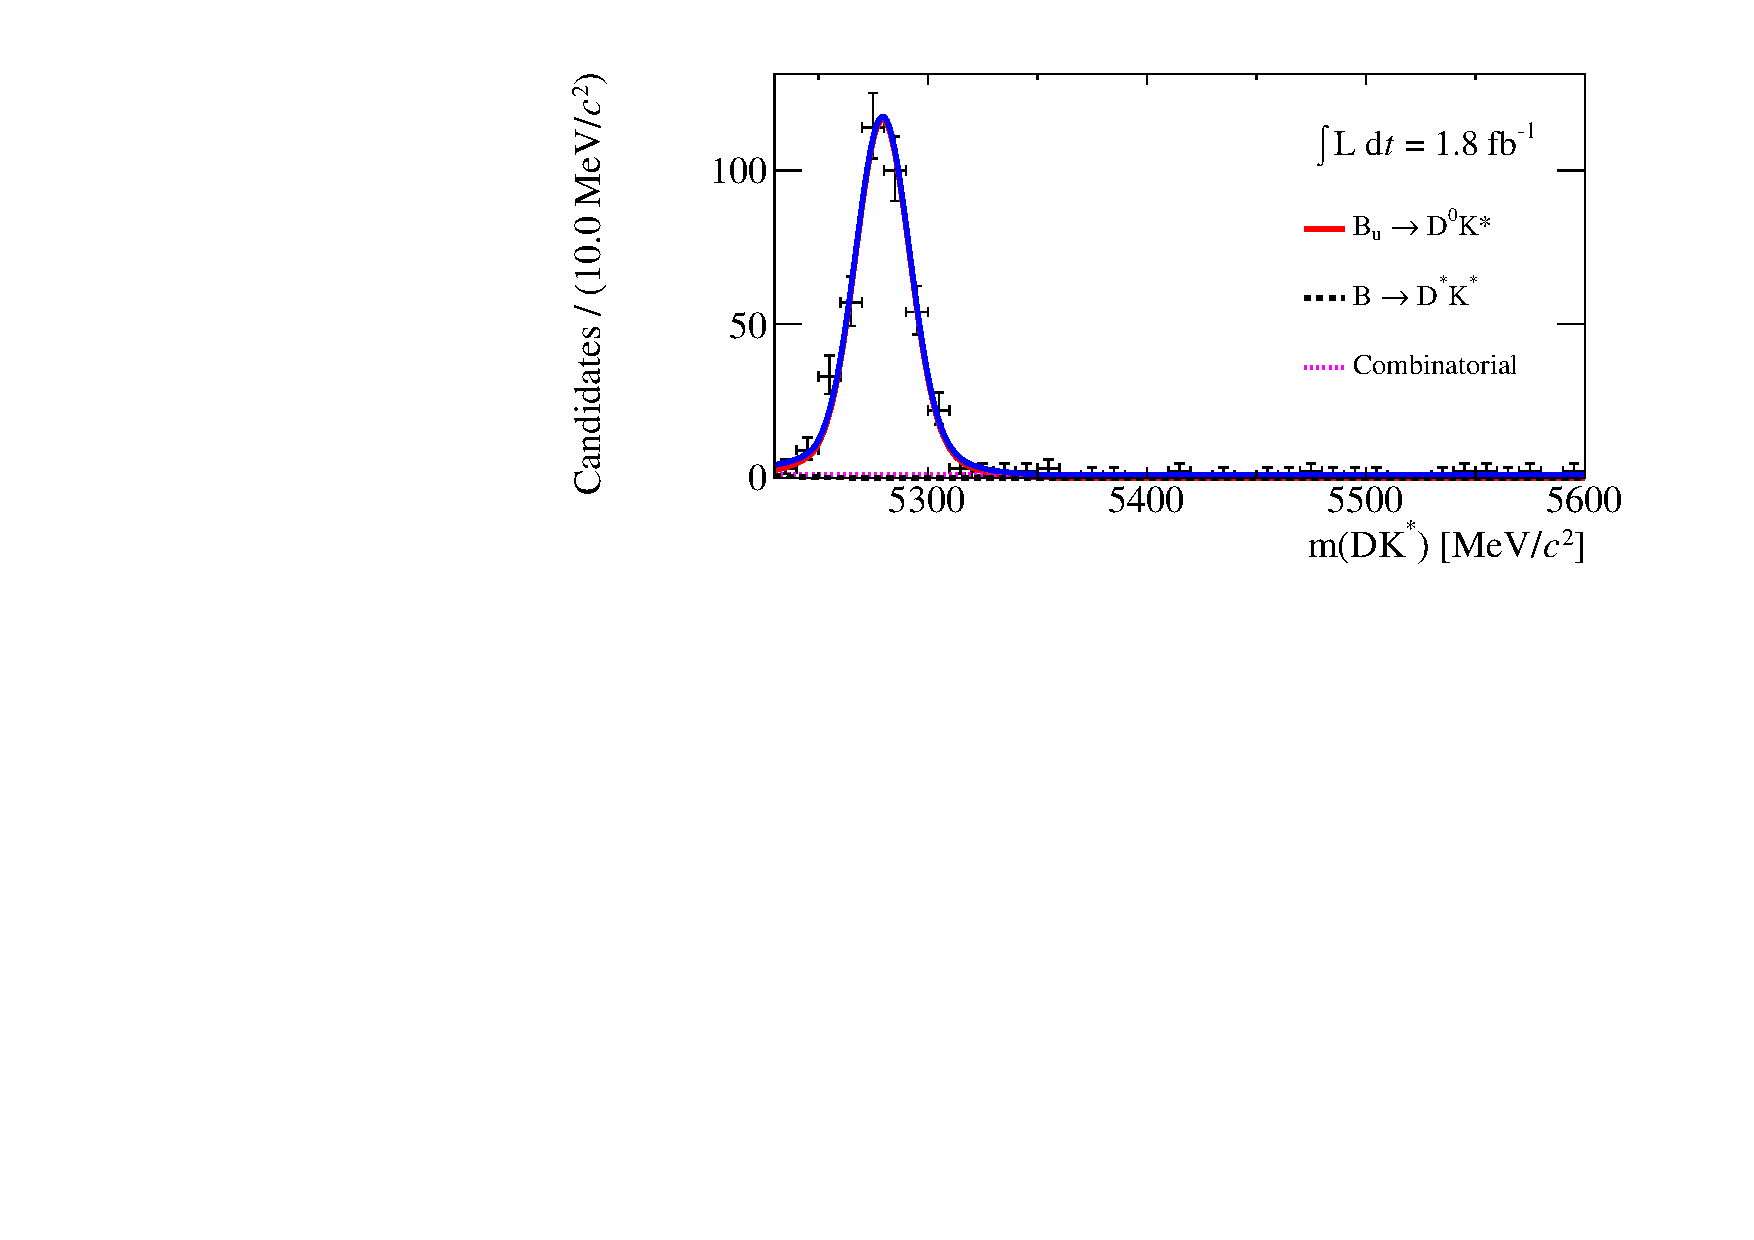
\includegraphics[width=0.25\linewidth]{combinedcanvas_d2kpi_LL_run2.pdf}}
%\hfill
%\subfloat[$KK$, LL]{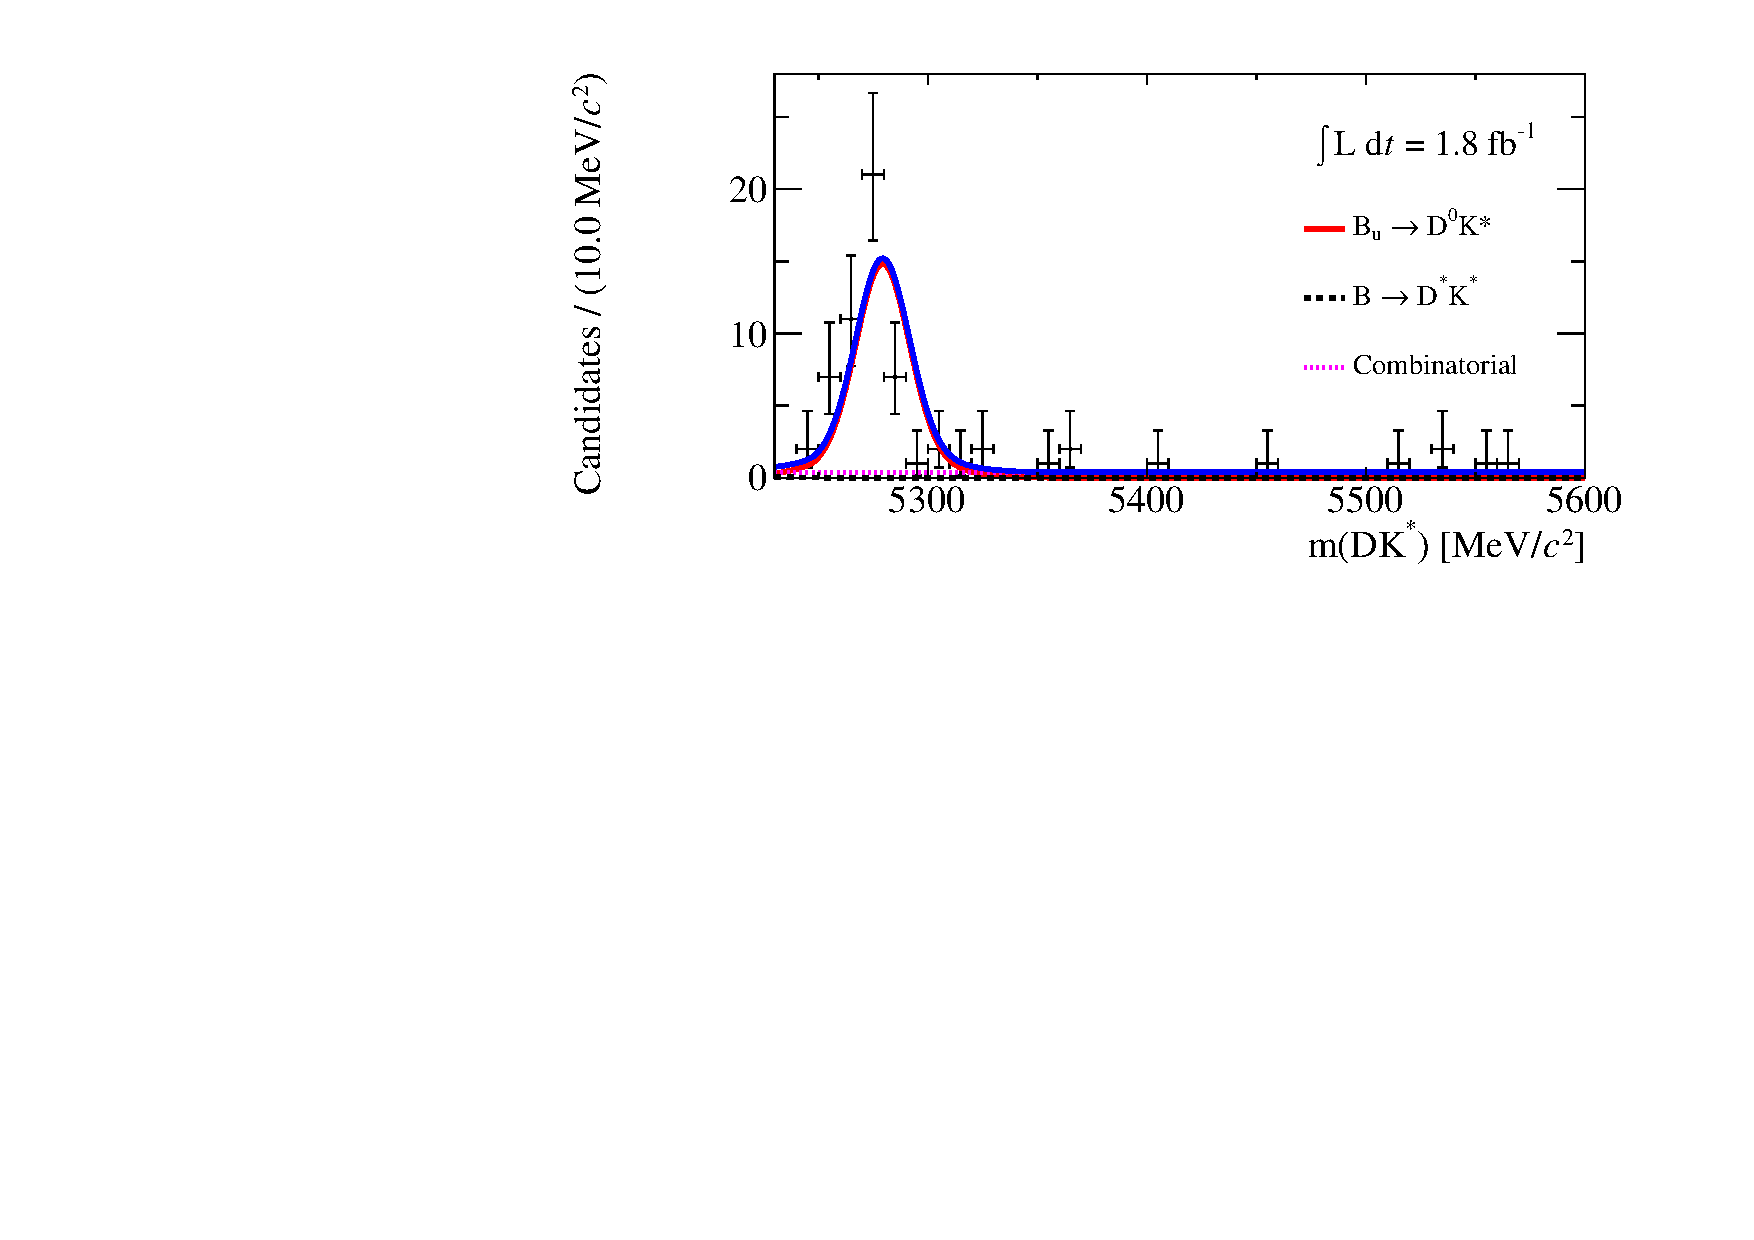
\includegraphics[width=0.25\linewidth]{combinedcanvas_d2kk_LL_run2.pdf}}
%\hfill
%\subfloat[$\pi\pi$, LL]{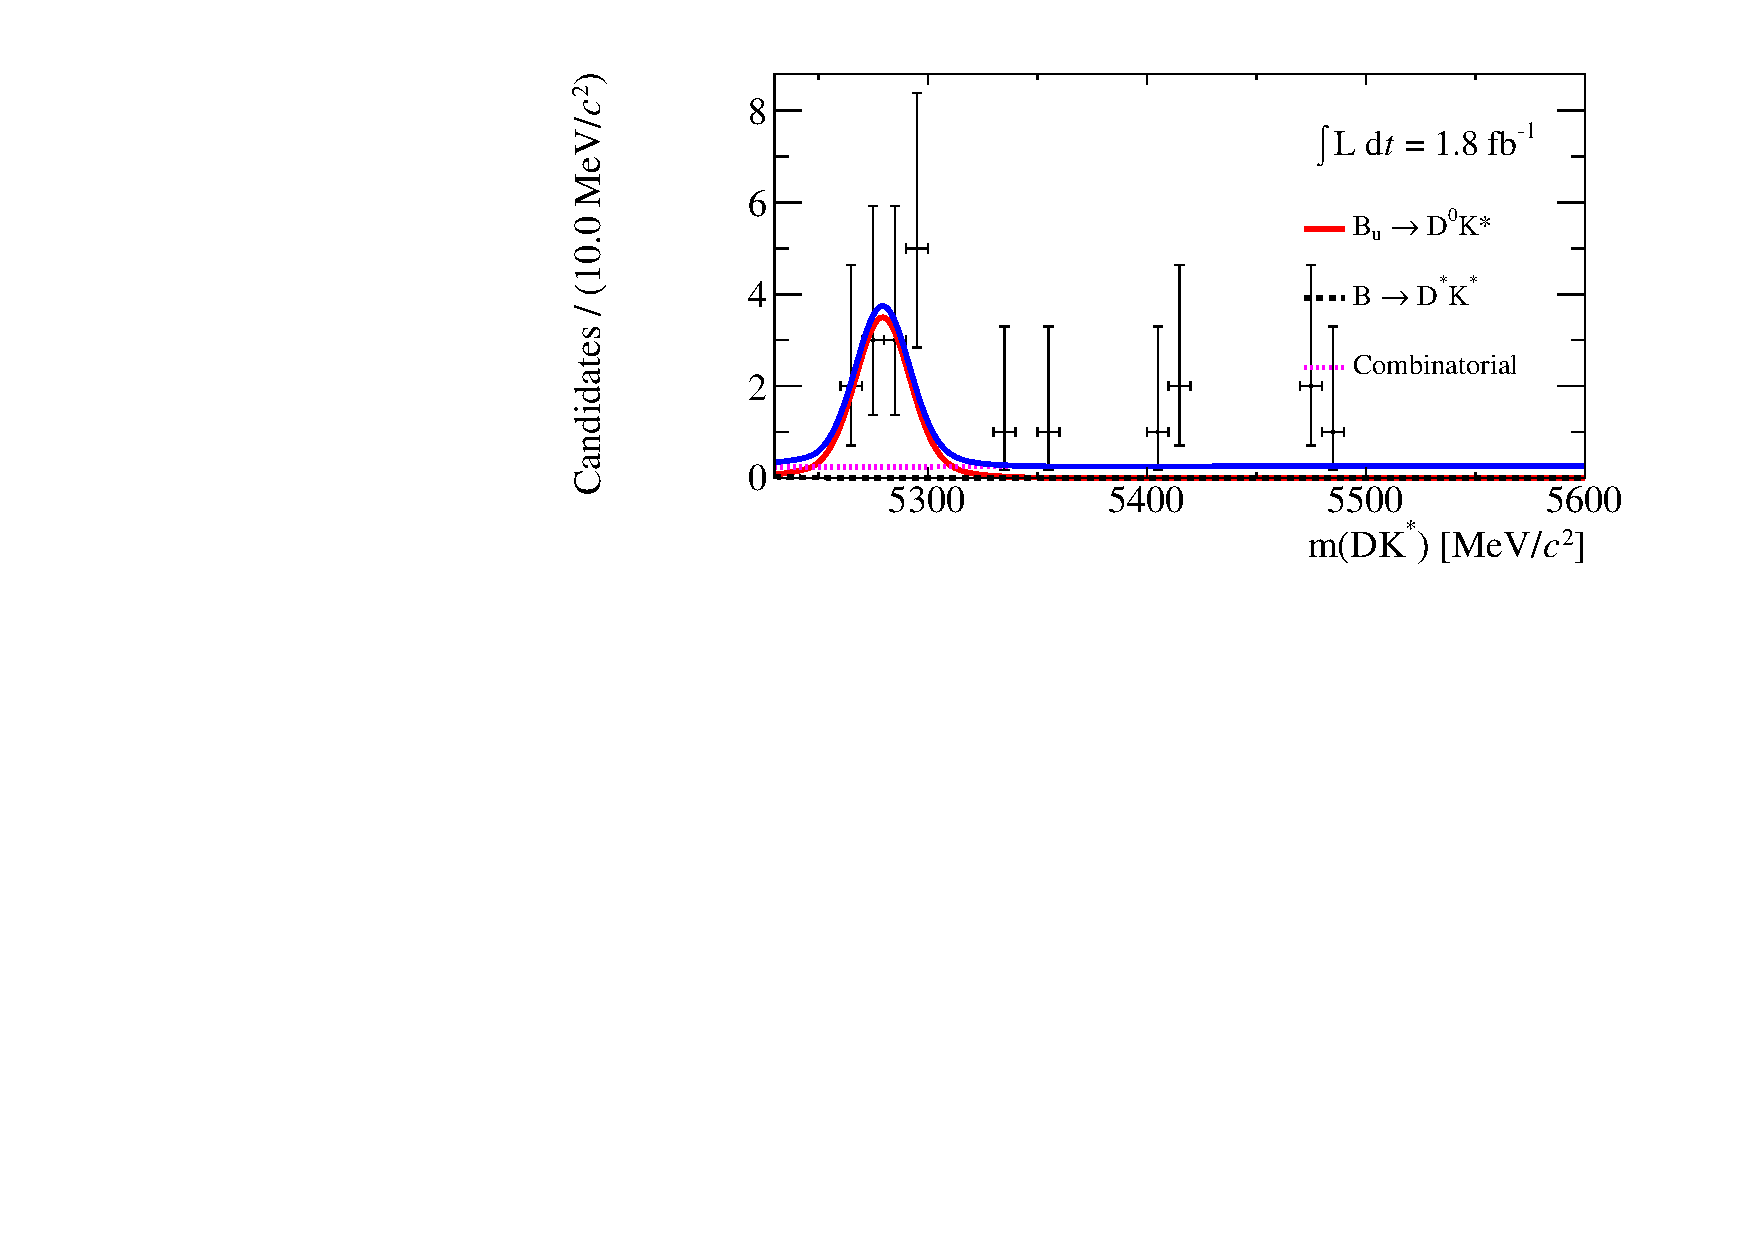
\includegraphics[width=0.25\linewidth]{combinedcanvas_d2pipi_LL_run2.pdf}}
%\hfill
%\subfloat[$\pi K$, LL]{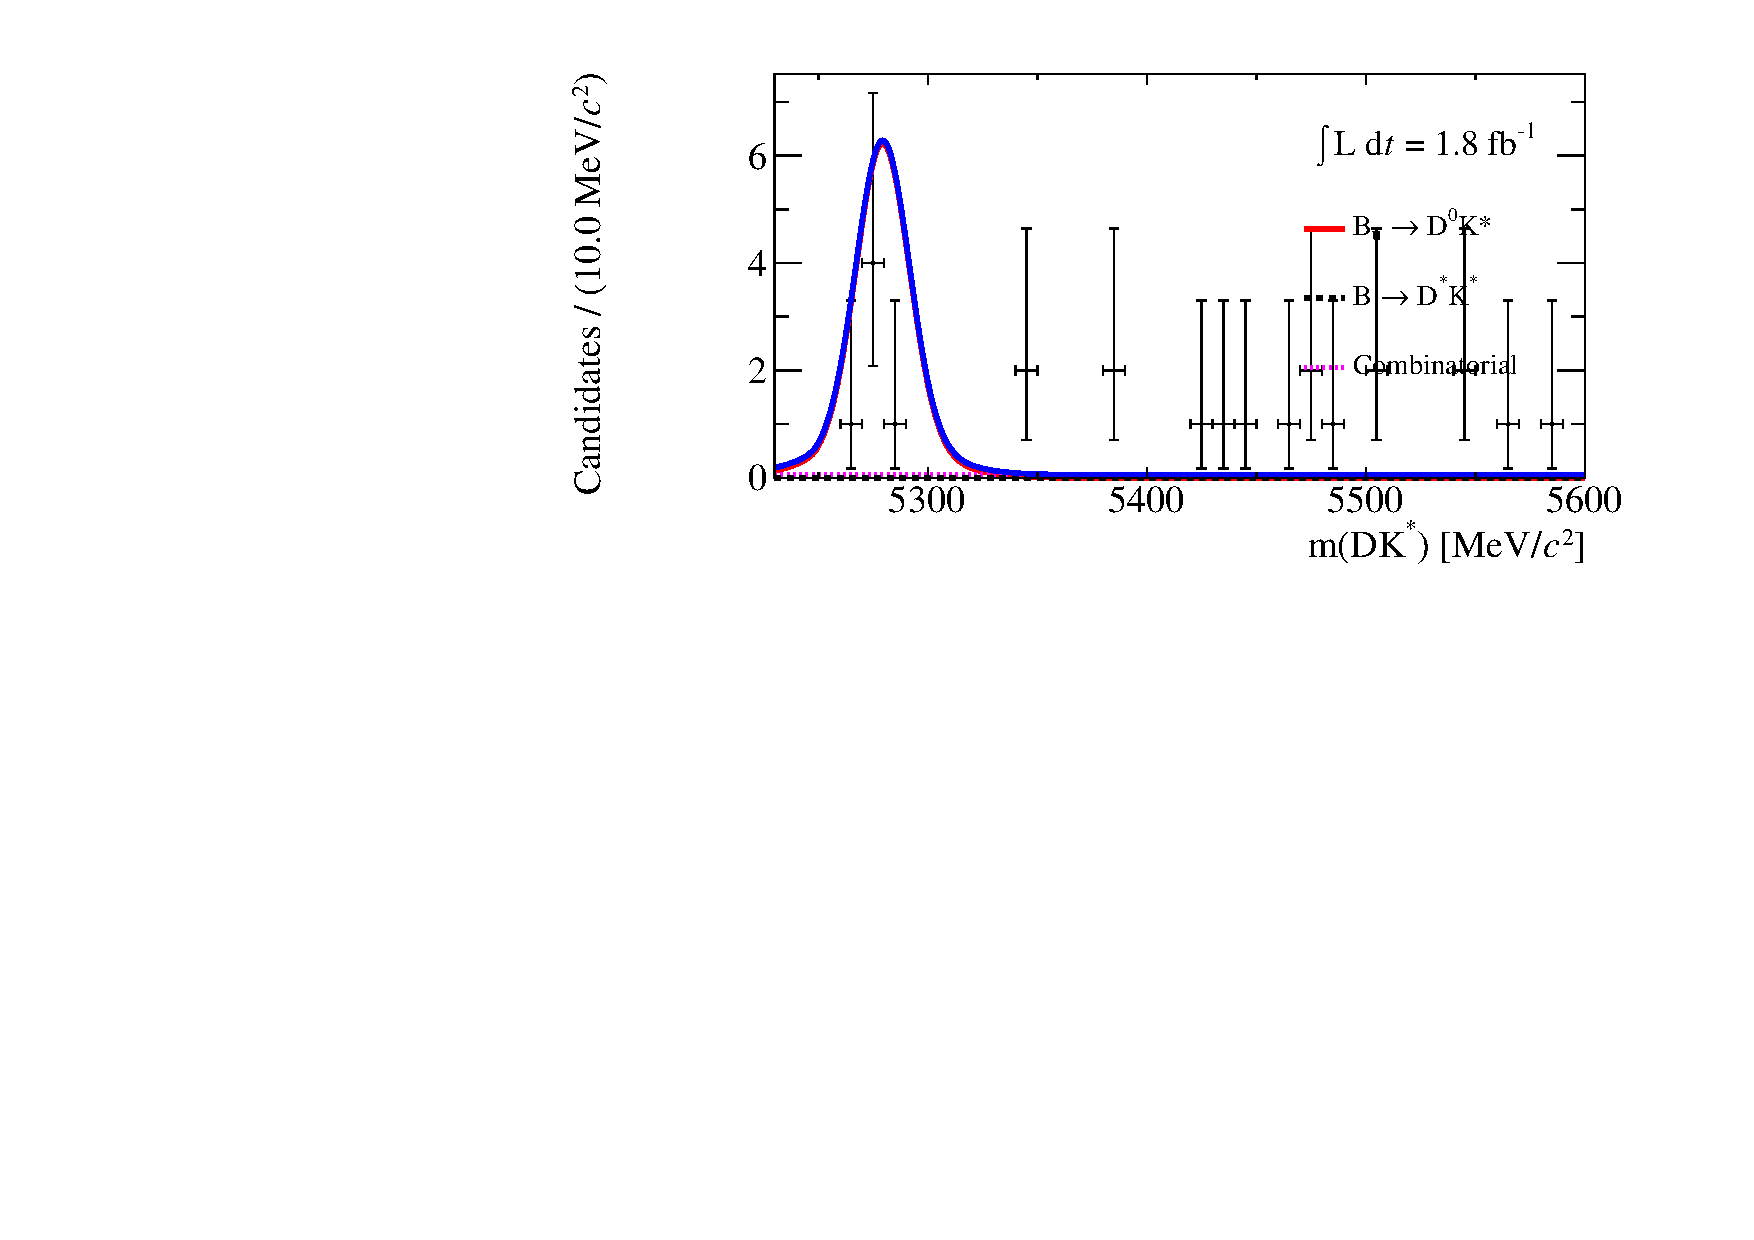
\includegraphics[width=0.25\linewidth]{combinedcanvas_d2pik_LL_run2.pdf}}
%\hfill
%\subfloat[$K\pi$, DD]{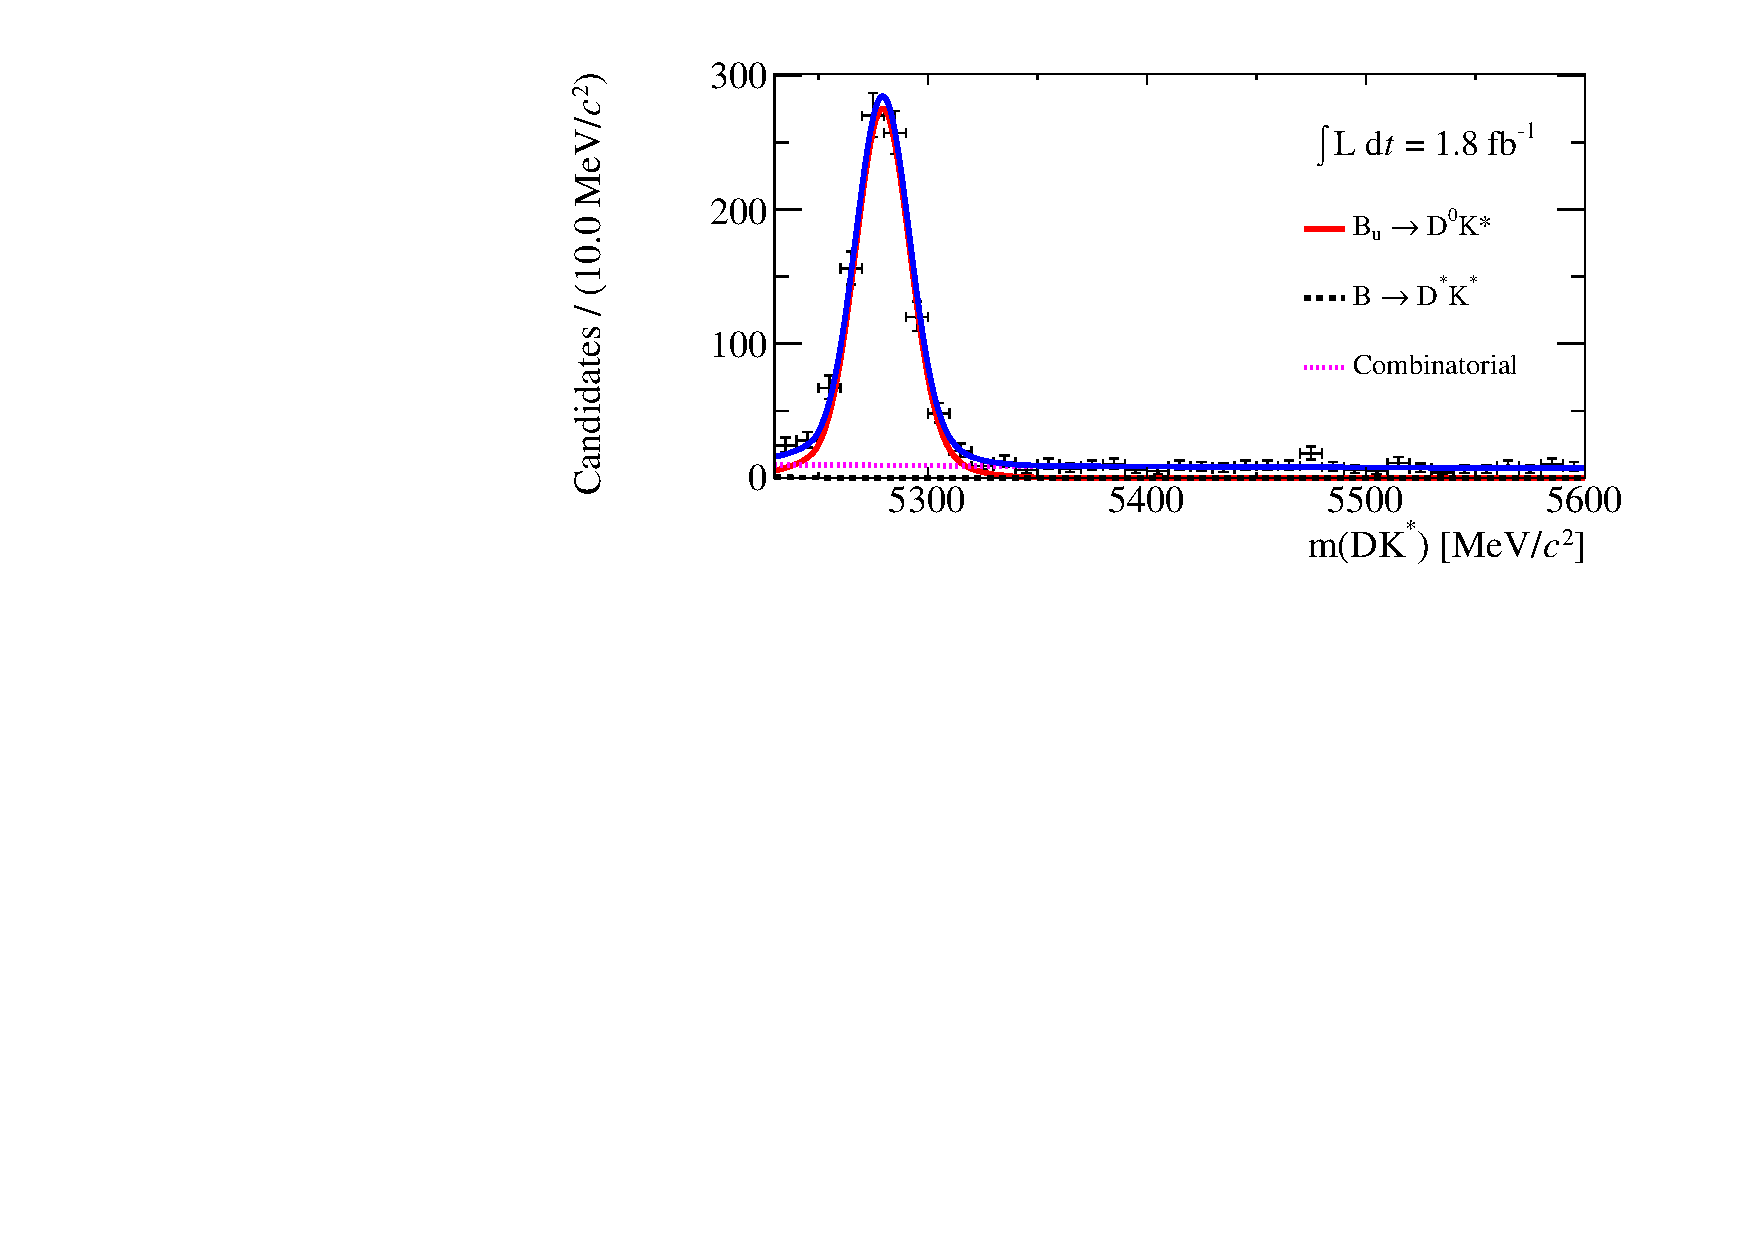
\includegraphics[width=0.25\linewidth]{combinedcanvas_d2kpi_DD_run2.pdf}}
%\hfill
%\subfloat[$KK$, DD]{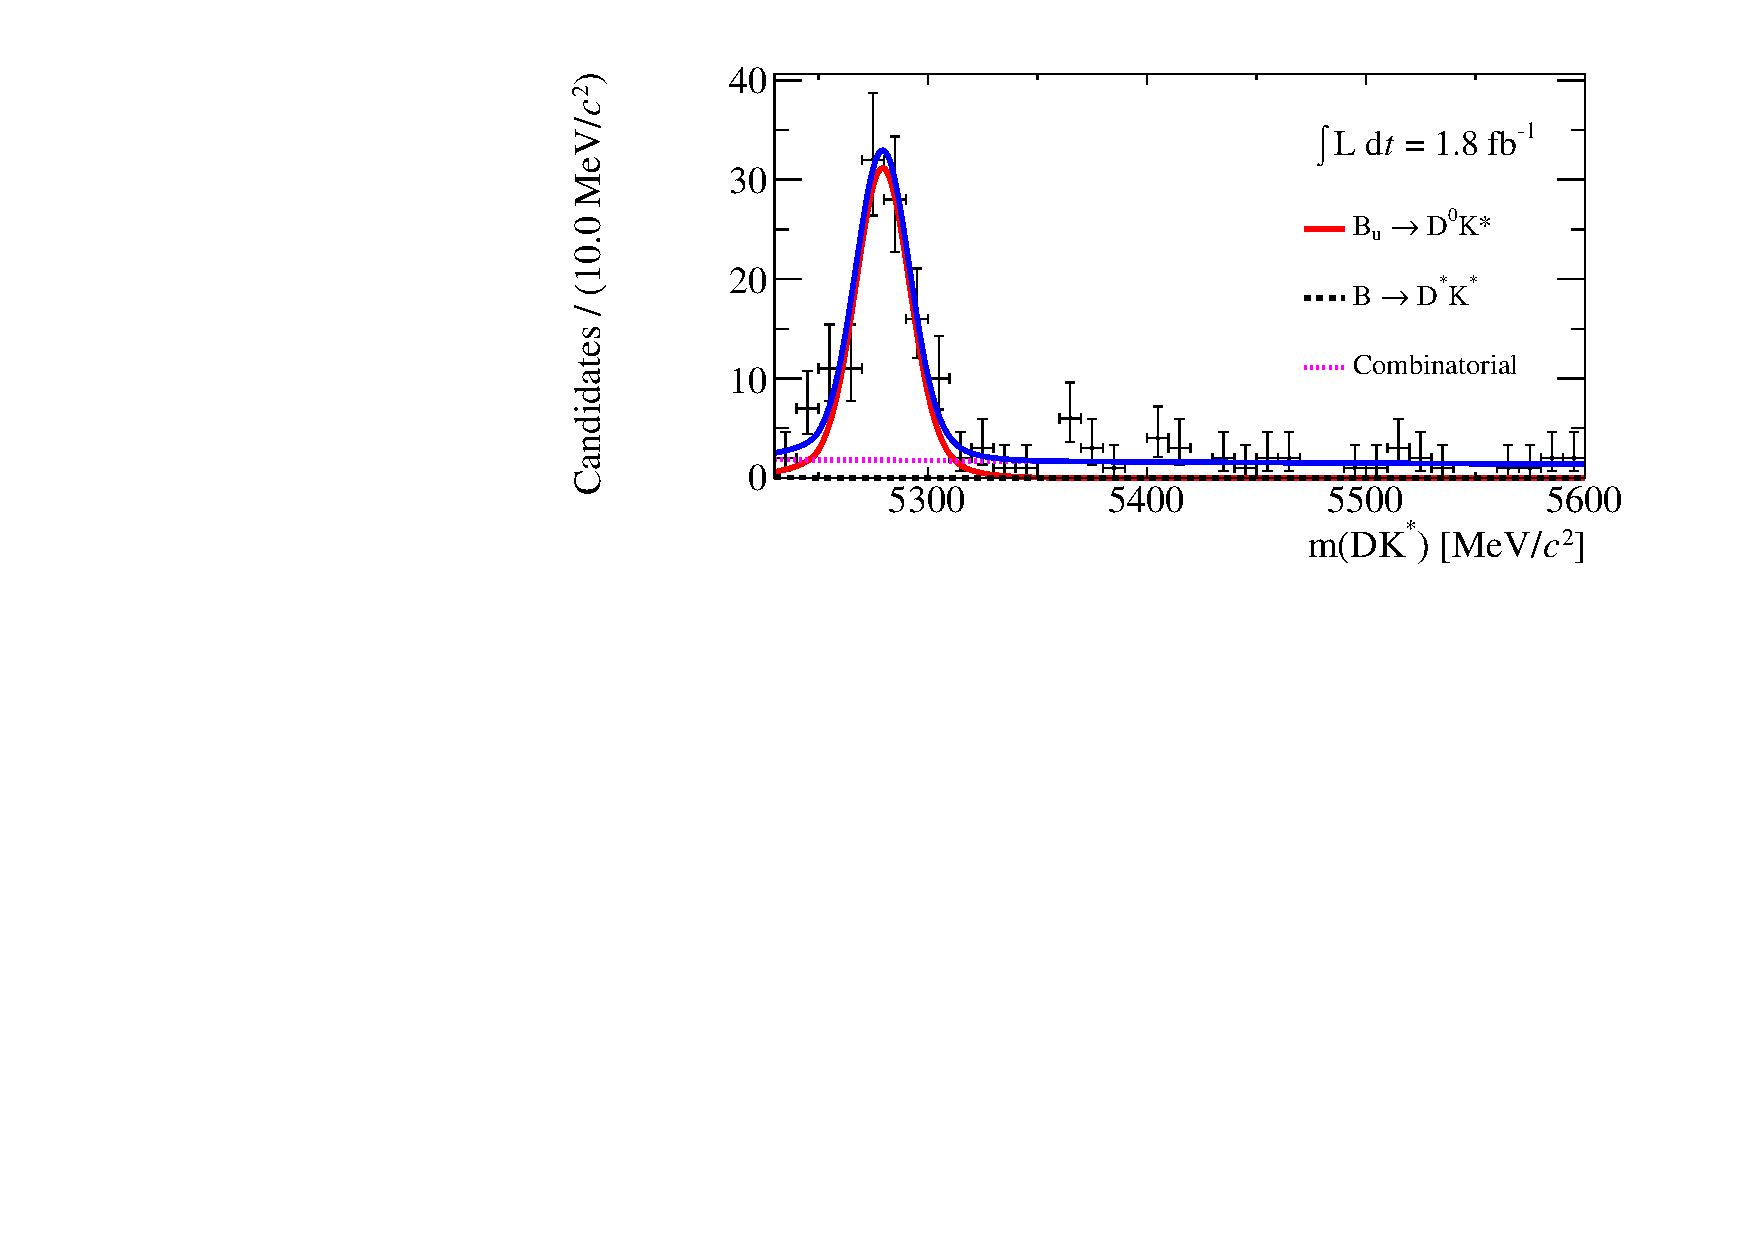
\includegraphics[width=0.25\linewidth]{combinedcanvas_d2kk_DD_run2.pdf}}
%\hfill
%\subfloat[$\pi\pi$, DD]{\includegraphics[width=0.25\linewidth]{combinedcanvas_d2pipi_DD_run2.pdf}}
%\hfill
%\subfloat[$\pi K$, DD]{\includegraphics[width=0.25\linewidth]{combinedcanvas_d2pik_DD_run2.pdf}}
%\hfill
%\subfloat[$K\pi\pi\pi$, LL]{\includegraphics[width=0.26\linewidth]{combinedcanvas_d2kpipipi_LL_run2.pdf}}
%\subfloat[$\pi\pi\pi\pi$, LL]{\includegraphics[width=0.26\linewidth]{combinedcanvas_d2pipipipi_LL_run2.pdf}}
%\subfloat[$\pi K\pi\pi$, LL]{\includegraphics[width=0.26\linewidth]{combinedcanvas_d2pikpipi_LL_run2.pdf}}
%\hfill
%\subfloat[$K\pi\pi\pi$, DD]{\includegraphics[width=0.26\linewidth]{combinedcanvas_d2kpipipi_DD_run2.pdf}}
%\subfloat[$\pi\pi\pi\pi$, DD]{\includegraphics[width=0.26\linewidth]{combinedcanvas_d2pipipipi_DD_run2.pdf}}
%\subfloat[$\pi K\pi\pi$, DD]{\includegraphics[width=0.26\linewidth]{combinedcanvas_d2pikpipi_DD_run2.pdf}}
%\caption{Results of the simultaneous fit for charged combined Run 2 data}
%\label{datafitcombinedRun2}
%\end{figure}

\begin{table}
\centering
\begin{tabular}{c|c}
\hline
\D mode & Total yield \\
\hline
$K\pi$ & $2030 \pm 49$ \\
$KK$ & $257 \pm 18$ \\
$\pi\pi$ & $80 \pm 11$ \\
$\pi K$ & $20 \pm 7$ \\
$K\pi\pi\pi$ & $1144 \pm 37$ \\
$\pi\pi\pi\pi$ & $115 \pm 13$ \\
$\pi K\pi\pi$ & $13 \pm 7$ \\
\hline
\end{tabular}
\caption{Total fitted yields in each of the \D decay modes from the charge combined fit}
\label{fittedyields}
\end{table}


%%%%%%%%%%%%%%%%%%%%%%%%

\subsection{Fitter bias in \CP fit}

Data was generated accoring to the model described in Section \ref{sec:massfit}, assuming yields taken from the single data fit to the favoured mode and \CP parameters were estimated assuming values of $r_B = 0.1$, $\delta_B = 111^o$ and $\gamma = 70^o$. The generated data was then fitted back using the same model and the fit parameters were extracted. This process was repeated 2000 times and the results are shown in Figures \ref{pulls1} and \ref{pulls2}. The quality of the fit is tested by observing the pull distribution of each fit parameter. The pull of a given parameter x is given by,

\begin{equation*}
P_x = \begin{cases}
	\frac{x_{fit} - x_{gen}}{\sigma_x^-}, & \text{if $x_{fit} - x_{gen} >$ 0}. \\
	\frac{x_{gen} - x_{fit}}{\sigma_x^+}, & \text{if $x_{fit} - x_{gen} <$ 0}.
	\end{cases}
\end{equation*}

where $x_{fit}$ is the value fo the parameter returned by the fit, $x_{gen}$ is the generated value of the parameter, and $\sigma_x^+$ and $\sigma_x^-$ are the upper and lower asymmetric errors respectively. All pull distributions are consistent with a mean of zero and width of 1. Therefore, the fit is considered stable and unbiased.
 
\begin{figure}[h]
\centering
\includegraphics[page=1,trim = 0mm 24mm 0mm 0mm,clip,width=0.8\linewidth]{figures/results/toys.pdf}
\includegraphics[page=2,trim = 0mm 165mm 0mm 10mm,clip,width=0.8\linewidth]{figures/results/toys.pdf}
\caption{Pulls of the physics observables in the fit. The left hand column shows the fitted parameter distribution, the middle shows the fit error distribution and the right most plots are the pull distributions fitted with a Gaussian.}
\label{pulls1}
\end{figure}

\begin{figure}[h]
\centering
\includegraphics[page=2,trim = 0mm 24mm 0mm 113mm,clip,width=0.8\linewidth]{figures/results/toys.pdf}
\includegraphics[page=3,trim = 0mm 165mm 0mm 10mm,clip,width=0.8\linewidth]{figures/results/toys.pdf}
\caption{Pulls of the physics observables in the fit. The left hand column shows the fitted parameter distribution, the middle shows the fit error distribution and the right most plots are the pull distributions fitted with a Gaussian.}
\label{pulls2}
\end{figure}

\subsection{Combinatoric background in ADS}
\label{sec:cpfit:comb}

One seemingly unexpected feature that is clear from Fig.~\ref{datafit2bodyRun1} is that the level of combinatoric background between the favoured $K\pi$ mode and ADS mode is different. Table \ref{adscombinatoric} compares the number of events between 5400 and 5600 MeV for $K\pi$ and $\pi K$ modes at different points in the selection. The numbers for the ADS mode with the full selection (after PID) do not have the tighter BDT cut or veto applied in order to be able to give a fairer comparison. Discrepancy seems to be present from the start but becomes larger with each stage of the selection, especially PID cuts. In the LL data the final level of combintoric background prior to the divergence in cuts is statistically compatible with being the same. In the DD sample the level of combinatoric (50 vs 14) is harder to attribute to a fluctuation, although the numbers involved are clearly quite small. A similar discrepacny can the seen in the 4-body favoured and suppressed mode, which is slightly less pronounced. It is noted that differences were also seen in the corresponding analysis of \decay{\Bm}{\D\Km}, $D\to K\pi\pi\pi$~\cite{LHCB-PAPER-2016-003}, but these were of order 2 rather than 3.5 as seen here. 

\begin{table}[h]
\centering
\begin{tabular}{l|ll|ll}
\hline
& \multicolumn{2}{c}{LL} & \multicolumn{2}{c}{DD} \\
& $K\pi$ & $\pi K$ & $K\pi$ & $\pi K$ \\
\hline
After stripping & 706538 & 686896 & 1064786 & 1019415 \\
+ pre-selection & 454 & 457 & 2792 & 2150 \\
+ BDT selection & 24 & 33 & 113 & 57 \\
+ PID selection & 10 & 8 & 50 & 14 \\
\hline
\end{tabular}
\caption{Comparison of the number of events between 5400 and 5600 MeV for $K\pi$ and $\pi K$ modes at different points in the selection.}
\label{adscombinatoric}
\end{table}

The decays being investigated, \decay{\Bm}{\D(\Km\pip)\Kstarm(\KS(\pip\pim)\pim)} and \decay{\Bm}{\D(\Km\pip\pim\pip)\Kstarm(\KS(\pip\pim)\pim)}, have a five and seven body final state respectively. The invariant mass sum of possible combinations of final state particles has been checked as well as various other background checks; these are shown in Appendix \ref{sec:app:combinatoric}. The results of this study remain inconclusive. Some differences in the distributions between the favoured and supressed modes are seen, as might be expected, however the majority of events used to make these plots would not be consistent with the $K^{*-}$ selection. We do learn that there are very few real $K^{*-}$ in the upper sideband, in either decay mode.

In the absence of futher information it is concluded that the rate of combinatoric background is due to the different pion charge combination. Hence in the favoured mode the pion from the \D and the bachelor pion have opposite sign, while in the ADS mode they have the same sign. This introduces a difference to the yield of combinatoric straight out of stripping which invovles very loose cuts.


\clearpage
